\documentclass[a4paper, 11pt]{report}
\usepackage[utf8]{inputenc}
\usepackage[spanish]{babel}
\usepackage{xcolor}
\usepackage{float}
\usepackage[hidelinks]{hyperref}
\usepackage[all]{hypcap}
\usepackage{bookmark}
\usepackage{graphicx}
\usepackage{emptypage}
\usepackage{eurosym}
\usepackage{geometry}
\usepackage[autopunct]{csquotes}
\usepackage{ragged2e}
\usepackage{longtable,tabularx,ltxtable,array}
\usepackage{multirow}
\usepackage{fancyhdr}
\usepackage{spreadtab}
\usepackage{fp}
\usepackage{changepage}
\usepackage{epigraph}
\usepackage{array}
\usepackage{lscape}
\usepackage{makecell}
\usepackage{enumitem}
\usepackage{svg}
\usepackage{amsmath}
\usepackage[Sonny]{fncychap}
\usepackage{nameref}
\usepackage{listings}
\usepackage{tocloft}
\usepackage{etoolbox}
\usepackage[bottom]{footmisc}
\usepackage[nottoc]{tocbibind}
\usepackage{booktabs}

\lstset{
  basicstyle=\ttfamily,
  columns=fullflexible,
  frame=single,
  breaklines=true,
  postbreak=\mbox{\textcolor{red}{$\hookrightarrow$}\space},
}

\newcommand\YAMLcolonstyle{\color{red}\mdseries}
\newcommand\YAMLkeystyle{\color{black}\bfseries}
\newcommand\YAMLvaluestyle{\color{blue}\mdseries}

\makeatletter

\newcommand\language@yaml{yaml}

\expandafter\expandafter\expandafter\lstdefinelanguage
\expandafter{\language@yaml}
{
  keywords={true,false,null,y,n},
  keywordstyle=\color{darkgray}\bfseries,
  basicstyle=\YAMLkeystyle,
  sensitive=false,
  comment=[l]{\#},
  morecomment=[s]{/*}{*/},
  commentstyle=\color{purple}\ttfamily,
  stringstyle=\YAMLvaluestyle\ttfamily,
  moredelim=[l][\color{orange}]{\&},
  moredelim=[l][\color{magenta}]{*},
  moredelim=**[il][\YAMLcolonstyle{:}\YAMLvaluestyle]{:},
  morestring=[b]',
  morestring=[b]",
  literate =    {---}{{\ProcessThreeDashes}}3
                {>}{{\textcolor{red}\textgreater}}1
                {|}{{\textcolor{red}\textbar}}1
                {\ -\ }{{\mdseries\ -\ }}3,
}

\lst@AddToHook{EveryLine}{\ifx\lst@language\language@yaml\YAMLkeystyle\fi}
\makeatother

\newcommand\ProcessThreeDashes{\llap{\color{cyan}\mdseries-{-}-}}

\renewcommand{\epigraphflush}{center}
\setlength{\epigraphwidth}{10cm}

\renewcommand{\cellalign}{\theadalign{cl}}
\renewcommand\theadfont{\bfseries}
\renewcommand\theadgape{\Gape[2pt]}
\renewcommand\cellgape{\Gape[2pt]}

\newcommand{\vsep}{\hfil\kern\arraycolsep\vline\kern-\arraycolsep\hfilneg}
\newcommand{\blankpage}
{
    \checkoddpage{}
    \ifoddpage{\newpage}{} \fi
    \cleardoublepage{}
    \thispagestyle{empty}
    \newpage
}

\newcommand{\DNI}{49340296Y}
\newcommand{\autor}{Guillermo López García}
\newcommand{\director}{Guadalupe Ortiz Bellot}
\newcommand{\codirector}{David Corral Plaza}
\newcommand{\proyecto}{Smart Rural}
\newcommand{\nombre}{Acrónimo proyecto}
\newcommand{\tipo}{Grado}
\newcommand{\titulo}{Ingeniería Informática}
\newcommand{\titulacion}{\tipo{} en \titulo}
\newcommand{\dia}{15}
\newcommand{\mes}{junio}
\newcommand{\anno}{2021}
\newcommand{\fecha}{\mes{} \anno}
\newcommand{\Fecha}{\dia{} de \mes{} de \anno}

\newcommand{\lorem}
{

}

\fancypagestyle{plain}
{
    \fancyhf{}
    \renewcommand{\headrulewidth}{0pt}
    \renewcommand{\footrulewidth}{0pt}
}

\fancypagestyle{prefacepage}
{
    \fancyhf{}
    \renewcommand{\headrulewidth}{0pt}
    \fancyfoot[RE,LO]{\textsl{\thepage}}

}

\fancypagestyle{chapterpage}
{
    \fancyhf{}
    \renewcommand{\headrulewidth}{0pt}
    \fancyfoot[RE,LO]{}
}

\setlength{\headheight}{15pt}
\fancyhead[LO]{\textbf{\textsl{\leftmark}}}
\fancyhead[LE]{\textbf{\textsl{\thepage}}}
\fancyhead[RO]{\textbf{\textsl{\thepage}}}
\fancyhead[RE]{\textbf{\textsl{\rightmark}}}
\fancyhead[C]{}

\fancyfoot[LE,RO]{}
\fancyfoot[LO,RE]{}
\fancyfoot[RE,LO]{}
\fancyfoot[RO,LE]{}
\fancyfoot[C]{}

\newenvironment{portada}
{
    \newgeometry{left=2cm,right=2cm,top=2cm,bottom=1cm}
    
\includegraphics[width=7cm, keepaspectratio]{images/UCA.jpg}  \\ \vspace{1cm}
    \begin{center}
}
{
    \end{center}
    \restoregeometry{}
}

\newcommand\addrow[2]{#1 &#2\\ }

\newcommand\addheading[2]{#1 &#2\\ \hline}
\newcommand\tabularhead{\begin{tabular}{lp{8cm}}
\hline
}

\newcommand\addmulrow[2]{ \begin{minipage}[t][][t]{2.5cm}#1\end{minipage}%
   &\begin{minipage}[t][][t]{8cm}
    \begin{enumerate} #2   \end{enumerate}
    \end{minipage}\\ }

\newenvironment{usecase}{\tabularhead}
{\hline\end{tabular}}

\begin{document}
    \begin{portada}
        \Large \MakeUppercase{Trabajo de Fin de Grado} \\ \vspace{1cm}
        \Large \MakeUppercase{\titulacion} \\ \vspace{6cm}
        \LARGE \MakeUppercase{\textbf{\proyecto}} \\ \vspace{7cm}
        \Large \MakeUppercase{Director: \director} \\
        \Large \MakeUppercase{Co-Director: \codirector} \\
        \Large \MakeUppercase{Autor: \autor} \\ \vspace{0.5cm}
        Puerto Real, \fecha{}
    \end{portada}

    \blankpage{}
    \pagenumbering{arabic}
    \pagestyle{fancy}
    \newenvironment{declaracion}
{
    \setlength{\parskip}{2em}
    \renewcommand{\baselinestretch}{1.25}
    \begin{center}
}
{
    \end{center}
    \restoregeometry{}
}

\begin{declaracion}
    \Large \MakeUppercase{\textbf{\underline{Declaración Personal de Autoría}}} \vspace{1.5cm}

    \justify{\normalsize{} \autor{} con DNI \DNI{}, estudiante del \titulacion{} en la Escuela Superior de Ingeniería de la Universidad de Cádiz,
    como autor de este documento academico, titulado \proyecto{} y presentado como trabajo final
    de \tipo{}.}

    \justify{\MakeUppercase{\normalsize{} Declaro que}}

    \justify{\normalsize Es un trabajo original, que no copio ni utilizo parte de obra alguna sin mencionar de
    forma clara su origen, tanto en el cuerpo del texto, como en su bibliografía, y que no
    empleo datos de terceros sin la debida autorización, de acuerdo con la legislación vigente.
    Así mismo, declaro que soy plenamente consciente de que no respetar esta obligación podrá
    implicar la aplicación de sanciones académicas, sin prejuicio de otras actuaciones que
    pudieran iniciarse.}


    \justify{\normalsize{} En Puerto Real, a \Fecha{} }\\ \vspace{2cm}


    \justify{\normalsize{} Fdo: \autor{}}
\end{declaracion}


    \blankpage{}

\thispagestyle{prefacepage}
{\large \textbf{\textit{Dedicatoria}}}
\vspace{0.5cm} \\
\lorem{}

\blankpage{}

\thispagestyle{prefacepage}
{\large \textbf{Notación y formato}} \smallskip
\vspace{0.5cm}\\
En la siguiente tabla se presenta un conjunto de convenios de notación de sintaxis.\smallskip
\vspace{0.5cm}
\begin{center}
    \begin{tabular}{|l|l|} \hline
        \multicolumn{2}{|c|}{Notación establecida} \\ \hline
        \textbf{negrita} & Título o texto destacado \\ \hline
        \textit{cursiva} & Texto en otro idioma, destacado, \\ & citas o nombres de aplicaciones \\ \hline
    \end{tabular}
\end{center}


    \blankpage

    \tableofcontents
    \chapter{Introducción}
    \section{Ámbito}
Actualmente, en el mundo rural, la tecnología no juega un gran papel, ya que, el trabajo en el campo se considera un trabajo anquilosado en el pasado, donde solo tiene cabida el trabajo manual pesado y la experiencia transmitida a lo largo de generaciones.

Con este proyecto, queremos cambiar esa situación, haciendo más ameno el trabajo manual al agricultor experimentado y facilitar la incorporación de personas jóvenes más familiarizada con las nuevas tecnologías.

Además, este proyecto está basado en necesidades expuestas por un grupo de agricultores, a los cuales se les ha consultado sobre si tuvieran la oportunidad de tener una aplicación para gestionar su trabajo rural, que le pedirían a dicha aplicación. Estos agricultores expusieron que les gustaría una aplicación accesible desde cualquier lado y que les guiará en temas de innovación sobre la agricultura y que les ayudará a automatizar tareas.

Por esto último, este proyecto usará las últimas tecnologías del mercado que permiten de forma nativa la capacidad multiplataforma. Así pues, usará el Software Deveploment Kit (SDK) Ionic \cite{ionic} con el FrameWork React \cite{react} para el Frontend \cite{frontend}. Como también, usará NodeJS \cite{nodejs} para la parte Backend \cite{backend} y Azure \cite{azure} para la integración de ambas partes con el Sistema de Internet de las Cosas (Internet of Things, IoT).

\section{Motivación}
La principal motivación que nos ha llevado a querer desarrollar este proyecto, ha sido la necesidad de mejorar la industrialización del medio rural, con lo que conlleva eso, es decir, la mejora en la productividad.

Además, facilitamos el acceso de personas de otros sectores a sector primario, ya que, con la herramienta propuesta, alivia mucho el trabajo sin ese conomiciento de generaciones del que hablamos en el anterior apartado.

También, nos motiva usar y aprender las últimas tecnologías en el mercado, donde con ellas generamos aplicaciones híbridas que usen la nube, en este caso, con la Plataforma como Servicio (Platform as a Service, PaaS) de Azure Cloud \cite{azure}.

Por último, una de las principales motivaciones a la hora de desarrollar este proyecto, ha sido la idea de innovar donde muy pocos investigadores lo han hecho, adaptar esas mismas innovaciones a un uso comercial y poder tener una alternativa en este sector tan competitivo donde tener una visión diferente en un momento dado, puede hacerte destacar y triunfar.

\section{Objetivos}
El objetivo de este TFG consiste en el diseño, desarrollo e implementación de, una aplicación hídrida que sirva como gestor de medios rurales al agricultor y de un Sistema de IoT con capacidad de detectar situaciones de interés, enviar alertas o notificaciones al usuario y de realizar las acciones automatizadas respecto a los mismos.

A su vez, este objetivo podríamos subdividirlo en distintos subojetivos más específicos. Estos son:

\begin{itemize}
    \item Gestionar los recursos rurales del agricultor a tráves de un dashboard web.
    \item Detectar situaciones de interés para el usuario.
    \item Notificar al usuario afectado mediante notificaciones o alertas en tiempo real.
    \item Tener un registro de todo lo que se ha comentado anteriormente y que se pueda consultar en todo momento desde un dashboard web.
\end{itemize}

\section{Alcance}
Este proyecto, es una aplicación híbrida (Web, Android, Desktop), para facilitar el acceso a la misma a todas las personas que quieran usarla en cualquier momento.

Las funcionalidades que tiene son:

\begin{itemize}
    \item Login: aquí el agricultor podrá loguearse en el sistema, entrar a su panel de dashboard y gestionar sus recursos.
    \item Gestionar Terrenos: aquí el agricultor podrá ver, añadir, actualizar y borrar los terrenos que posea, junto con sus caracteristicas.
    \item Gestionar Cultivos: aquí el agricultor podrá ver, añadir, actualizar y borrar los cultivos de un terreno.
    \item Gestionar Fitosanitarios: aquí el agricultor podrá ver, añadir, actualizar y borrar los fitosanitarios añadidos a un cultivo.
    \item Gestionar Riegos: aquí el agricultor podrá ver, añadir, actualizar y borrar los riegos sobre un terreno.
    \item Gestionar Eventos: aquí el agricultor podrá suscribirse/dessuscribirse a un evento complejo y podrá decidir que tipo de acción se ejecute una vez el evento se dispare.
    \item Notificaciones: aquí el agricultor podrá ver todo el listado de notificaciones que ha recibido en el tiempo, ordenados de más cercano a mas lejano.
    \item Ajustes: aquí el agricultor podrá cambiar ciertos ajustes de su perfil, tales como Modo Claro / Modo Oscuro (Look and Feel), Idioma o Acción por defecto en los eventos complejos.
    \item Búsqueda por palabras coincidentes: el agricultor podrá buscar en cada sección del dashboard para así filtrar por las palabras clave que el desee.
\end{itemize}

\section{Estructura de la memoria}
La actual memoria se divide en los siguientes capítulos:
\begin{itemize}
    \item 1. Introducción: En este capítulo se expone la motivación para la realización del trabajo fin de grado actual, el alcance del mismo, el enfoque metodológico aplicado para la realización del mismo y un glosario con los acrónimos usados en la presente memoria.
    \item 2. Conceptos preliminares y estado del arte: En este capítulo se mostrarán aplicaciones y herramientas similares. Explicando lo que aporta la presente aplicación desarrollada respecto a las ya existentes.
    \item 3. Planificación del proyecto: En este capítulo se mostrará el enfoque metodológico usado. Así como la investigación previa, los diagramas Gantt usados para la planificación de actividades y proyecto finalizado.
    \item 4. Análisis del sistema: En este capítulo se mostrarán los objetivos del sistema, los actores y los requisitos tanto funcionales, como no funcionales del sistema.
    \item 5. Diseño del sistema: En este capítulo mostraremos los distintos modelos de datos.
    \item 6. Implementación del sistema: En este capítulo se expondrá las distintas tecnologías usadas para el desarrollo del sistema actual incluyendo enlaces al repositorio de Github donde se encontrará el código fuente.
    \item 7. Pruebas del sistema: En este capítulo se detallará las diferentes pruebas usadas para la verificación del sistema.
    \item 8. Manual de instalación: En este capítulo se explicará como desplegar el sistema en el cloud de Azure, los requisitos previos del sistema y como instalar el software en los distintos dispositivos.
    \item 9. Manual de usuario: En este capítulo se explicará como puede usar el software el usuario, tanto el acceso al mismo como el manejo del software para su óptimo funcionamiento.
    \item 10. Conclusión: En este capítulo pondremos en común los conocimientos adquiridos tras el desarrollo del proyecto. También, se expondrán las mejoras futuras y los objetivos cumplidos tras el desarrollo del mismo.
\end{itemize}
    \chapter{Conceptos preliminares y estado del arte}
    En este capítulo definiremos lo que es un proyecto de SmartRural usando diferentes definiciones, mostrando proyectos que están relacionados con el entorno del medio rural y comparandolas con nuestro proyecto.

\newpage

El término SmartRural surgió hace unos años como sinónimo del proyecto europeo Smart Village \cite{smart-village} (aldea inteligente), con el ánimo de añadir tecnologías TIC al mundo rural para optimizar el trabajo y por ende, aumentar la productividad y los beneficios al explotar los cultivos.

Respecto a esto último, solo queda añadir como dato que actualmente hay en total como unos 21 pueblos seleccionados en toda la Unión Europea (UE), para sumarse a este cambio digital y están supervisados por 28 expertos, uno por cada país miembro, y coordinados a nivel superior por E40 Group \cite{e40group} con socios como IfLS and empirica \cite{ifls} (Alemania), Innovatiesteunput \cite{innovatiesteunput} (Bélgica), Agricultural University of Athens \cite{greece} (Grecia) and eConcepts \cite{econcepts} (Irlanda).

A parte del proyecto europeo con subvención de la misma Unión Europea, existe un proyecto que merece especial atención y que se basa en mezclar tecnología informática con el medio rural. Este es Smart Rural \cite{smart-rural} (Agricultura Inteligente). 

Este proyecto, surgió en 2015 en Castilla y León, con la idea de mejorar mediante la tecnología, la Agricultura de Precisión. A parte, este proyecto contiene un sistema de gestión de recursos agrícolas y una bitacora para indicar que ha ido bien, que ha ido mal y posibles mantenimientos a realizar en distintas zonas.

Como dato a añadir a esto último, Smart Rural se ha convertido en una empresa respetable tanto dentro del sector de la tecnología, como del sector de la agricultura. Tiene presencia en países europeos y en países de hispanoamérica, como Chile o Argentina, y además ha recibido distintivos premios como ``Premio a la mejor empresa innovadora ADE2020'' (2015), ``Premio al emprendimiento por Aranda Emprende'' (2015), ``Premio Hermano Celestino'' (2016) y ``Premio a la innovación en Infoagro Exhibition'' (2019) \cite{team-smartrural}.

A continuación, en la Figura 2.1, se puede observar la página web principal de la empresa Smart Rural.

\begin{figure}[H]
    \centering
    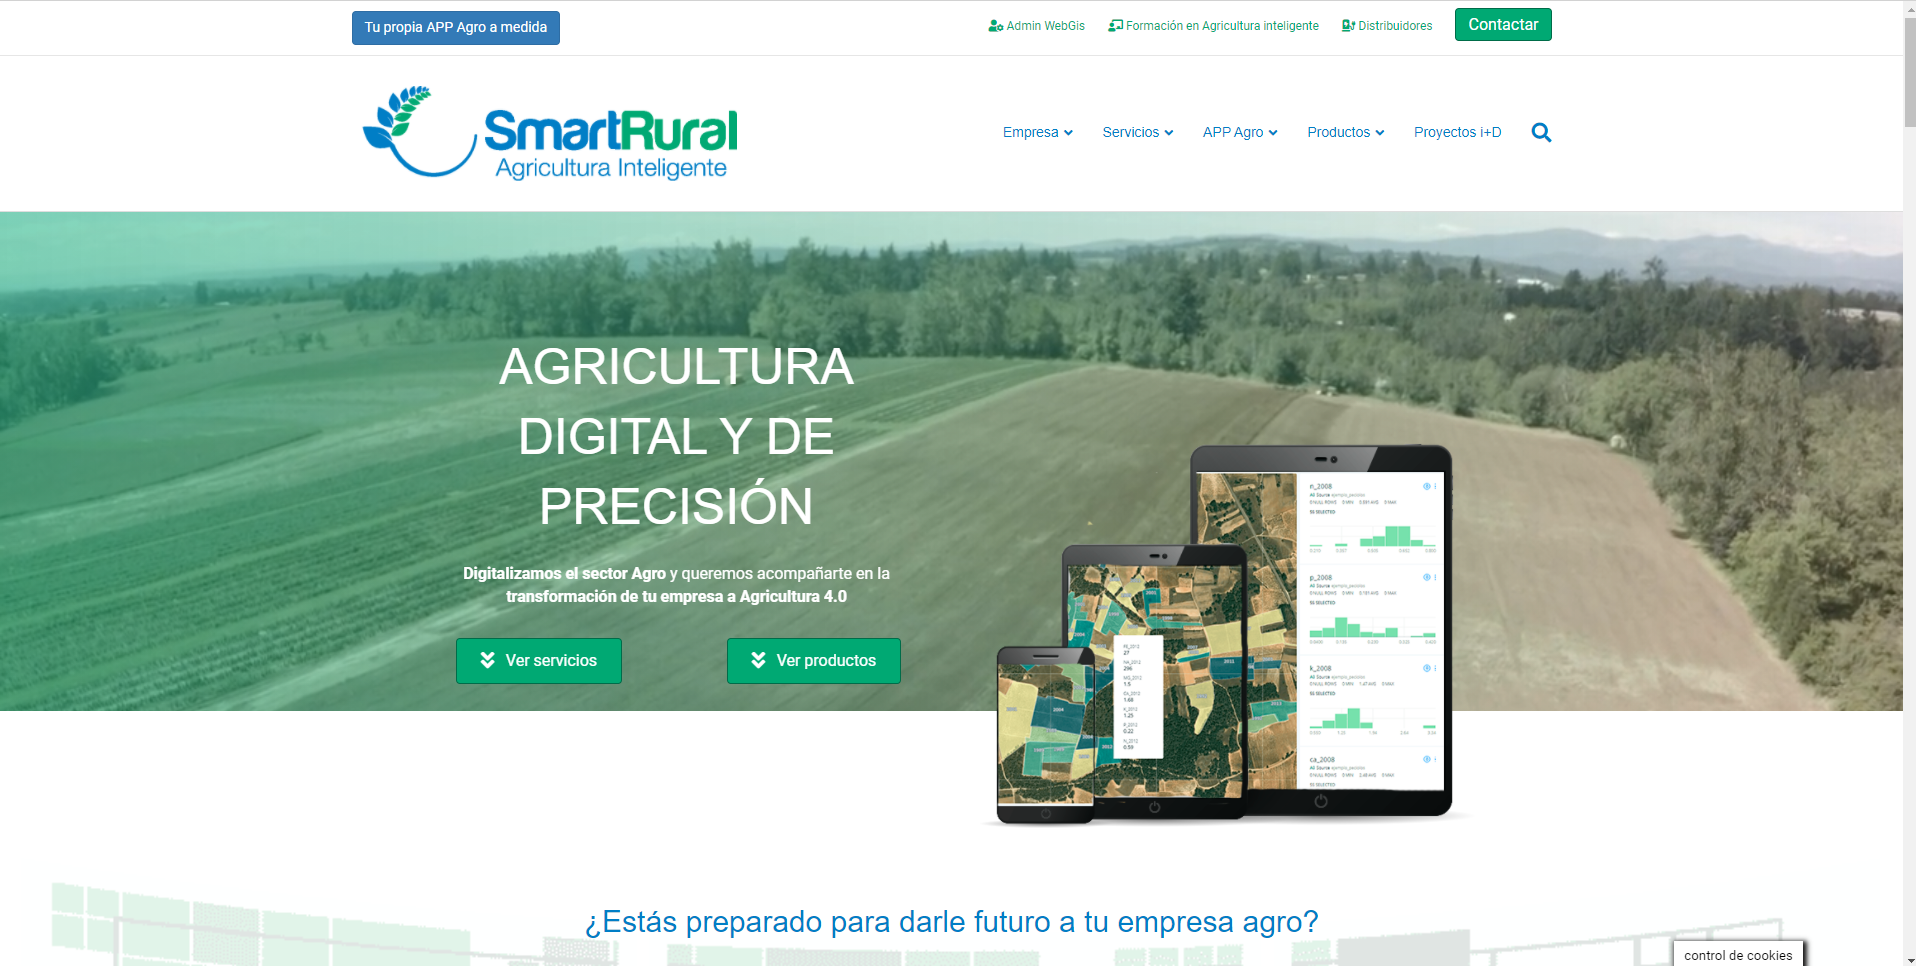
\includegraphics[width=0.85\linewidth]{images/state-art/smartrural.png}
    \caption{https://smartrural.net/}
\end{figure}

Nuestra aplicación tiene un ámbito parecida a la expuesta anteriormente, pero con un cambio significativo. Nuestro proyecto tendrá capacidad multiplataforma gracias al SDK de Ionic y Azure Cloud, además que añadimos un Sistema de IoT para detección de eventos, apostando por el desarrollo de aplicaciones híbridas y programación reactiva.

Además, ofrecemos almacenamiento online gracias a la perfecta integración que tienen estas tecnologías híbridas con las nubes de computación públicas existentes, tanto Azure Cloud para el procesamiento de datos como Amazon Web Services con su Relational Database Service para guardar los datos.

Por último, ofrecemos una tabla, Cuadro 2.1, con la comparativa entre el proyecto europeo, Smart Rural y nuestro proyecto, para identificar de forma breve y sencilla las diferencias entre la competencia y nosotros.

\begin{table}[!htbp]
    \centering
    \resizebox{\textwidth}{!}{
        \begin{tabular}{rlllrrrrr}
        \hline
            Características & Smart Village & Smart Rural & Nuestro proyecto \\
        \hline
            Integración Nube & No & No & Sí \\
            Aplicaciones Móviles & No & Sí & Sí \\
            Detección de Eventos & No & No & Sí \\
            Gestor de Recursos & No & Sí & Sí \\
            Interconectividad entre plataformas & Sí & Sí & Sí \\
            Sistema de IoT & No & No & Sí \\
            Sistemas de Gráficos y Estadísticas & Sí & Sí & No \\
            Sistema de Marketing Digital & No & Sí & No \\
        \hline
        \end{tabular}
    }
    \caption{Tabla comparativa}
\end{table}


    \chapter{Planificación}
    En este capítulo se mostrará el enfoque metodológico usado. Así como los riesgos, los recursos disponibles y los diagramas Gantt usados para la planificación de actividades y proyecto finalizado.

\newpage

\section{Investigación previa}
Debido a que a la gran mayoría de las necesidades actuales de cualquier aplicación que ofrezca un servicio necesita un servicio en la nube para almacenar datos, y con el estudio previo de la única implementación con éxito de un Sistema de SmartRural, decidimos escoger tecnologías híbridas que nos permitieran un desarrollo rápido, de caracter multiplataforma y escalable con el tiempo.

Así pues, para nuestro proyecto, escogimos el SDK Ionic, ya que, tiene una gran integración con la metología ágil y la PaaS de Azure Cloud.

\section{Enfoque metodológico}
Para el desarrollo de nuestro proyecto, hemos escogido la metodología ágil, por su gran versátilidad y la obligación al mismo tiempo de establecer ciclos iterativos donde se puedan sacar hitos del producto y así llegar mejor al producto final deseado.

Por ende, dentro de la metodología ágil, usaremos el más ampliamente usado, es decir, Scrum \cite{scrum}.

Por último, y para garantizar el éxito del proyecto, se han realizado revisiones periodicas por nuestra parte del producto en cada iteración, tanto de su dirección como de su calidad funcional y de implementación (Clean Code \cite{cleancode}\cite{cleancodebook}).

\section{Planificación del proyecto}
En este apartado, mostraremos el procedimiento de desarrollo de los componentes en 4 fases dentro de cada hito. Estas son:

\begin{itemize}
    \item Análisis: en esta fase vamos a definir los requisitos funcionales y no funcionales que forma el sistema dentro del hito. Después, los añadiremos a un Backlog para su posterior desarrollo.
    \item Diseño: en esta fase diseñaremos los prototipos de nuestro sistema y sus correspondientes diagramas conceptuales.
    \item Implementación: en esta fase implementaremos las tareas provenientes en el Backlog. Queda aclarar que muchas de las funcionalidades descritas en el Backlog tiene parte de implementación en el Backend y otra parte en el Frontend, así ha sido necesario el desarrollo de ambas partes al unisono para conseguir el funcionamiento deseado.
    \item Pruebas: por último, en esta fase se han desarrollado pruebas unitarias tanto en el Backend como en el Frontend. Se han omitido pruebas de integración, de aceptación, ...etc por qué con el software actual, no se han considerado necesarias.
\end{itemize}

\section{Diagrama Gantt}
En esta sección, mostraremos el diagrama de Gantt final de la ejecución del proyecto, que incluirá estimaciones iniciales más retrasos propios de no haber hecho en su momento bien las estimaciones o por circunstancias especiales. A continuación, en la Figura 3.1, se muestra el diagrama de Gantt.

\begin{figure}[H]
    \centering
    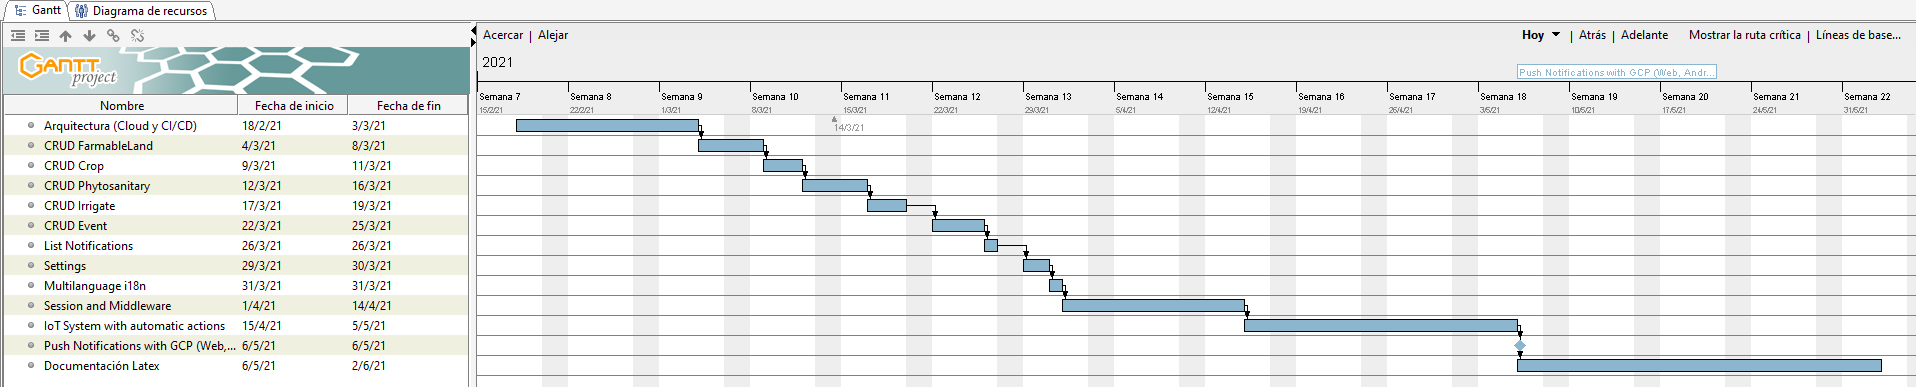
\includegraphics[width=1\linewidth,angle=90]{images/state-art/gantt.png}
    \caption{Estimaciones + Tiempo real de ejecución}
\end{figure}
    \chapter{Análisis}
    En este capítulo se realiza un estudio desde los requerimientos necesarios y profundizando las necesidades de la misma para cumplir con los objetivos que se esperan.

\newpage

\section{Requisitos}
En este apartado se indican los requisitos para el sistema a implementar. Así conseguiremos identificar las necesidades del mismo. Esto también nos servira para corroborar el cumplimiento de los requisitos establecidos.

En los siguientes apartados, mostraremos los requisitos funcionales, los requisitos no funcionales, los requisitos de información y los distintos diagramas de casos de uso.

\section{Objetivos del sistema}
A continuación, describimos los objetivos del sistema:

\begin{table}[!htbp]
    \centering
    \resizebox{\textwidth}{!}{
        \begin{tabular}{p{4cm} | p{10cm}}
          \hline
            OBJ-0001 & Acceso al sistema \\
          \hline
            Descripción & Se deberá controlar el acceso al sistema, mediante un sistema
                          de login y el cual a parte de permitir el acceso a las pantallas
                          de gestión, deberá controlar a nivel de petición el login. \\
           \hline
        \end{tabular}
    }
    \caption{OBJ-0001}
\end{table}

\begin{table}[!htbp]
    \centering
    \resizebox{\textwidth}{!}{
        \begin{tabular}{p{4cm} | p{10cm}}
          \hline
            OBJ-0002 & Gestionar Terrenos \\
          \hline
            Descripción & Se deberá permitir leer, borrar, crear y actualizar los
                          terrenos disponibles \\
           \hline
        \end{tabular}
    }
    \caption{OBJ-0002}
\end{table}

\begin{table}[!htbp]
    \centering
    \resizebox{\textwidth}{!}{
        \begin{tabular}{p{4cm} | p{10cm}}
          \hline
            OBJ-0003 & Gestionar Cultivos \\
          \hline
            Descripción & Se deberá permitir leer, borrar, crear y actualizar los
                          cultivos en los terrenos disponibles \\
           \hline
        \end{tabular}
    }
    \caption{OBJ-0003}
\end{table}

\begin{table}[!htbp]
    \centering
    \resizebox{\textwidth}{!}{
        \begin{tabular}{p{4cm} | p{10cm}}
          \hline
            OBJ-0004 & Gestionar Fitosanitarios \\
          \hline
            Descripción & Se deberá permitir leer, borrar, crear y actualizar los fitosanitarios                     aplicados a los cultivos de los terrenos disponibles \\
           \hline
        \end{tabular}
    }
    \caption{OBJ-0004}
\end{table}

\begin{table}[!htbp]
    \centering
    \resizebox{\textwidth}{!}{
        \begin{tabular}{p{4cm} | p{10cm}}
          \hline
            OBJ-0005 & Gestionar Riegos \\
          \hline
            Descripción & Se deberá permitir leer, borrar, crear y actualizar los
                          riegos sobre terrenos disponibles \\
           \hline
        \end{tabular}
    }
    \caption{OBJ-0005}
\end{table}

\begin{table}[!htbp]
    \centering
    \resizebox{\textwidth}{!}{
        \begin{tabular}{p{4cm} | p{10cm}}
          \hline
            OBJ-0006 & Gestionar Suscripción a Eventos Complejos \\
          \hline
            Descripción & Se deberá permitir la suscripción al evento complejo que se quiera
                          y escoger la acción a hacer por defecto cuando el evento complejo
                          se realiza. \\
           \hline
        \end{tabular}
    }
    \caption{OBJ-0006}
\end{table}

\begin{table}[!htbp]
    \centering
    \resizebox{\textwidth}{!}{
        \begin{tabular}{p{4cm} | p{10cm}}
          \hline
            OBJ-0007 & Consultar las notificaciones \\
          \hline
            Descripción & Se deberá permitir consultar el histórico de las notificaciones
                          del usuario, respecto a los eventos lanzados. \\
           \hline
        \end{tabular}
    }
    \caption{OBJ-0007}
\end{table}

\begin{table}[!htbp]
    \centering
    \resizebox{\textwidth}{!}{
        \begin{tabular}{p{4cm} | p{10cm}}
          \hline
            OBJ-0008 & Modificar el idioma de la aplicación \\
          \hline
            Descripción & Se deberá permitir la elección del idioma en la aplicación.
                          En concreto, entre castellano o inglés. \\
           \hline
        \end{tabular}
    }
    \caption{OBJ-0008}
\end{table}

\begin{table}[!htbp]
    \centering
    \resizebox{\textwidth}{!}{
        \begin{tabular}{p{4cm} | p{10cm}}
          \hline
            OBJ-0009 & Modificar la acción por defecto en eventos \\
          \hline
            Descripción & Se deberá permitir la elección del tipo de acción por defecto
                          en los eventos complejos. En concreto, entre Manual o Automático. \\
           \hline
        \end{tabular}
    }
    \caption{OBJ-0009}
\end{table}

\begin{table}[!htbp]
    \centering
    \resizebox{\textwidth}{!}{
        \begin{tabular}{p{4cm} | p{10cm}}
          \hline
            OBJ-0010 & Modificar el look and feel de la aplicación \\
          \hline
            Descripción & Se deberá permitir la elección del aspecto de la aplicación,
                          en concreto la elección será entre modo claro o modo oscuro. \\
           \hline
        \end{tabular}
    }
    \caption{OBJ-0010}
\end{table}

\begin{table}[!htbp]
    \centering
    \resizebox{\textwidth}{!}{
        \begin{tabular}{p{4cm} | p{10cm}}
          \hline
            OBJ-0011 & Búsqueda por palabras coincidentes \\
          \hline
            Descripción & Se deberá permitir en cada sección buscar y filtrar por palabras clave. \\
           \hline
        \end{tabular}
    }
    \caption{OBJ-0011}
\end{table}

\newpage

\section{Catálogo de actores}
En este apartado, mostraremos todos los actores implicados en el uso de la aplicación:

\begin{table}[!htbp]
    \centering
    \resizebox{\textwidth}{!}{
        \begin{tabular}{p{4cm} | p{10cm}}
          \hline
            ACT-001 & Usuario habitual \\
          \hline
            Descripción & Este usuario es el usuario final, es decir, el cliente. Dicho usuario
                          puede usar toda la aplicación en su totalidad. Es decir, tiene todos
                          los privilegios en el front-office. \\
           \hline
        \end{tabular}
    }
    \caption{OBJ-0011}
\end{table}

\section{Requisitos funcionales}
A continuación, exponemos los requisitos funcionales de nuestro sistema:

\begin{table}[!htbp]
    \centering
    \resizebox{\textwidth}{!}{
        \begin{tabular}{p{4cm} | p{10cm}}
          \hline
            UC-001 & Inicio de Sesión \\
          \hline
            Descripción & El sistema deberá mostrar el comportamiento que se describe a continuación
                          cuando un usuario desee iniciar sesión para acceder al sistema \\
            Precondición & El usuario debe existir con la contraseña especificada y con permisos para                 poder hacer el login \\
            Secuencia Normal (S) & 1. El sistema muestra la pantalla para iniciar sesión \\
                                 & 2. El usuario introduce sus credenciales en el formulario \\
                                 & 3. El sistema verifica que existe el usuario y que la contraseña es      correcta y muestra la pantalla principal del sistema. \\
            Postcondición & El usuario tiene la sesión iniciada con un tiempo máximo de una hora. \\
            Excepciones & 1. El usuario no existe y por tanto, el sistema da un error. \\
                        & 2. La contraseña no coincide con la del usuario, y por tanto el sistema
                             da un error. \\
           \hline
        \end{tabular}
    }
    \caption{UC-001}
\end{table}

\begin{table}[!htbp]
    \centering
    \resizebox{\textwidth}{!}{
        \begin{tabular}{p{4cm} | p{10cm}}
          \hline
            UC-002 & Cerrar Sesión \\
          \hline
            Descripción & El sistema deberá mostrar el comportamiento que se describe a continuación
                          cuando un usuario desee cerrar sesión para salir del sistema \\
            Precondición & El usuario debe existir y debe estar logueado. \\
            Secuencia Normal (S) & 1. El sistema muestra la pantalla principal del sistema \\
                                 & 2. El usuario pulsa la opción llamada ``Cerrar sesión'' \\
                                 & 3. El sistema detecta el cierre de sesión y expulsa al usuario
                                      del sistema \\
            Postcondición & El usuario tiene la sesión cerrada y ya no puede acceder al sistema \\
            Excepciones & 1. El usuario no tiene conexión a internet, y por tanto, la petición de
                             cerrar sesión no funciona. \\
           \hline
        \end{tabular}
    }
    \caption{UC-002}
\end{table}

\begin{table}[!htbp]
    \centering
    \resizebox{\textwidth}{!}{
        \begin{tabular}{p{4cm} | p{10cm}}
          \hline
            UC-003 & Listar Terrenos \\
          \hline
            Descripción & El sistema deberá mostrar el comportamiento que se describe a continuación
                          cuando un usuario desee listar sus terrenos \\
            Precondición & El usuario debe existir y debe estar logueado. \\
            Secuencia Normal (S) & 1. El sistema muestra la pantalla principal del sistema \\
                                 & 2. El usuario pulsa la opción llamada ``Terrenos'' \\
                                 & 3. El sistema detecta la petición y muestra los terrenos
                                      asociados al usuario. \\
            Postcondición & El usuario tiene un listado en la pantalla de sus terrenos asociados \\
            Excepciones & 1. El usuario no tiene conexión a internet, y por tanto, la petición
                             no funciona. \\
                        & 2. El usuario no tiene terrenos asociados, y por tanto, aparece un
                             listado vacío. \\
           \hline
        \end{tabular}
    }
    \caption{UC-003}
\end{table}

\begin{table}[!htbp]
    \centering
    \resizebox{\textwidth}{!}{
        \begin{tabular}{p{4cm} | p{10cm}}
          \hline
            UC-004 & Buscar Terrenos \\
          \hline
            Descripción & El sistema deberá mostrar el comportamiento que se describe a continuación
                          cuando un usuario desee buscar sus terrenos \\
            Precondición & El usuario debe existir y debe estar logueado. \\
            Secuencia Normal (S) & 1. El sistema muestra la pantalla principal del sistema \\
                                 & 2. El usuario pulsa la opción llamada ``Terrenos'' \\
                                 & 3. El usuario pulsa en el icono con forma de lupa \\
                                 & 4. El sistema detecta la petición y muestra los terrenos
                                      asociados al usuario que coinciden con la búsqueda. \\
            Postcondición & El usuario tiene un listado en la pantalla de sus terrenos asociados \\
            Excepciones & 1. El usuario no tiene conexión a internet, y por tanto, la petición
                             no funciona. \\
                        & 2. El usuario no tiene terrenos asociados, y por tanto, aparece un
                             listado vacío. \\
                        & 3. El usuario no tiene terrenos asociados que coincidan con la búsqueda,
                             y por tanto, aparece un listado vacío. \\
           \hline
        \end{tabular}
    }
    \caption{UC-004}
\end{table}

\begin{table}[!htbp]
    \centering
    \resizebox{\textwidth}{!}{
        \begin{tabular}{p{4cm} | p{10cm}}
          \hline
            UC-005 & Añadir Terreno \\
          \hline
            Descripción & El sistema deberá mostrar el comportamiento que se describe a continuación
                          cuando un usuario desee añadir un terreno \\
            Precondición & El usuario debe existir y debe estar logueado. \\
            Secuencia Normal (S) & 1. El sistema muestra la pantalla principal del sistema \\
                                 & 2. El usuario pulsa la opción llamada ``Terrenos'' \\
                                 & 3. El usuario pulsa en el icono con el símbolo ``+'' \\
                                 & 4. El sistema detecta la petición y muestra la pantalla
                                      de añadir terreno \\
                                 & 5. El usuario completa todos los campos y pulsa el botón de
                                      ``Añadir Terreno'' \\
            Postcondición & El usuario tiene un listado de sus terrenos con el terreno que acaba
                            de añadir \\
            Excepciones & 1. El usuario no tiene conexión a internet, y por tanto, la petición
                            no funciona. \\
                        & 2. El usuario no ha introducido de forma correcta algunos de los campos
                             y por tanto, la petición falla. \\
           \hline
        \end{tabular}
    }
    \caption{UC-005}
\end{table}

\begin{table}[!htbp]
    \centering
    \resizebox{\textwidth}{!}{
        \begin{tabular}{p{4cm} | p{10cm}}
          \hline
            UC-006 & Modificar Terreno \\
          \hline
            Descripción & El sistema deberá mostrar el comportamiento que se describe a continuación
                          cuando un usuario desee modificar un terreno \\
            Precondición & El usuario debe existir y debe estar logueado. \\
            Secuencia Normal (S) & 1. El sistema muestra la pantalla principal del sistema \\
                                 & 2. El usuario pulsa la opción llamada ``Terrenos'' \\
                                 & 3. El usuario pulsa en el icono con el símbolo de edición de
                                      color azul \\
                                 & 4. El sistema detecta la petición y muestra la pantalla
                                      de editar terreno \\
                                 & 5. El usuario modifica los campos que quiera y pulsa el botón de
                                      ``Modificar Terreno'' \\
            Postcondición & El usuario tiene un listado de sus terrenos con el terreno que acaba
                            de editar \\
            Excepciones & 1. El usuario no tiene conexión a internet, y por tanto, la petición
                             no funciona. \\
                        & 2. El usuario no ha introducido de forma correcta algunos de los campos
                             y por tanto, la petición falla. \\
           \hline
        \end{tabular}
    }
    \caption{UC-006}
\end{table}

\begin{table}[!htbp]
    \centering
    \resizebox{\textwidth}{!}{
        \begin{tabular}{p{4cm} | p{10cm}}
          \hline
            UC-007 & Borrar Terreno \\
          \hline
            Descripción & El sistema deberá mostrar el comportamiento que se describe a continuación
                          cuando un usuario desee borrar un terreno \\
            Precondición & El usuario debe existir y debe estar logueado. \\
            Secuencia Normal (S) & 1. El sistema muestra la pantalla principal del sistema \\
                                 & 2. El usuario pulsa la opción llamada ``Terrenos'' \\
                                 & 3. El usuario pulsa en el icono con el símbolo de borrado de
                                      color rojo \\
                                 & 4. El sistema detecta la petición, borra el terreno y
                                      actualiza el listado de terrenos \\
            Postcondición & El usuario tiene un listado de sus terrenos sin el terreno que acaba
                            de borrar \\
            Excepciones & 1. El usuario no tiene conexión a internet, y por tanto, la petición
                             no funciona. \\
           \hline
        \end{tabular}
    }
    \caption{UC-007}
\end{table}

\begin{table}[!htbp]
    \centering
    \resizebox{\textwidth}{!}{
        \begin{tabular}{p{4cm} | p{10cm}}
          \hline
            UC-008 & Listar Cultivos \\
          \hline
            Descripción & El sistema deberá mostrar el comportamiento que se describe a continuación
                          cuando un usuario desee listar los cultivos de sus terrenos \\
            Precondición & El usuario debe existir y debe estar logueado. \\
            Secuencia Normal (S) & 1. El sistema muestra la pantalla principal del sistema \\
                                 & 2. El usuario pulsa la opción llamada ``Cultivos'' \\
                                 & 4. El sistema detecta la petición, y lista los cultivos asociados
                                      a cualquier de sus terrenos \\
            Postcondición & El usuario tiene un listado de los cultivos de cualquiera de sus terrenos \\
            Excepciones & 1. El usuario no tiene conexión a internet, y por tanto, la petición
                             no funciona. \\
                        & 2. El usuario no tiene ningún terreno asociado y por tanto, el listado
                             aparece vacío. \\
                        & 3. El usuario no tiene ningún cultivo asociado y por tanto, el listado
                             aparece vacío. \\
           \hline
        \end{tabular}
    }
    \caption{UC-008}
\end{table}

\begin{table}[!htbp]
    \centering
    \resizebox{\textwidth}{!}{
        \begin{tabular}{p{4cm} | p{10cm}}
          \hline
            UC-009 & Buscar Cultivos \\
          \hline
            Descripción & El sistema deberá mostrar el comportamiento que se describe a continuación
                          cuando un usuario desee buscar los cultivos de sus terrenos \\
            Precondición & El usuario debe existir y debe estar logueado. \\
            Secuencia Normal (S) & 1. El sistema muestra la pantalla principal del sistema \\
                                 & 2. El usuario pulsa la opción llamada ``Cultivos'' \\
                                 & 3. El usuario pulsa en el icono con forma de lupa \\
                                 & 4. El usuario escribe la búsqueda que desea \\
                                 & 5. El sistema detecta la petición, y lista los cultivos asociados
                                      a cualquier de sus terrenos que coincida con la búsqueda \\
            Postcondición & El usuario tiene un listado de los cultivos de cualquiera de sus terrenos \\
            Excepciones & 1. El usuario no tiene conexión a internet, y por tanto, la petición
                             no funciona. \\
                        & 2. El usuario no tiene ningún terreno asociado y por tanto, el listado
                             aparece vacío. \\
                        & 3. El usuario no tiene ningún cultivo asociado y por tanto, el listado
                             aparece vacío. \\
                        & 4. El usuario no tiene ninguún cultivo o terreno que coincida con la
                             búsqueda \\
           \hline
        \end{tabular}
    }
    \caption{UC-009}
\end{table}

\begin{table}[!htbp]
    \centering
    \resizebox{\textwidth}{!}{
        \begin{tabular}{p{4cm} | p{10cm}}
          \hline
            UC-010 & Añadir Cultivo \\
          \hline
            Descripción & El sistema deberá mostrar el comportamiento que se describe a continuación
                        cuando un usuario desee añadir un cultivo a un terreno \\
            Precondición & El usuario debe existir y debe estar logueado. \\
            Secuencia Normal (S) & 1. El sistema muestra la pantalla principal del sistema \\
                                 & 2. El usuario pulsa la opción llamada ``Cultivos'' \\
                                 & 3. El usuario pulsa en el icono con el símbolo ``+'' \\
                                 & 4. El usuario selecciona el cultivo y el terreno que desea añadir \\
                                 & 5. El sistema detecta la petición y añadir el cultivo al terreno
                                      deseado \\
            Postcondición & El usuario tiene un listado de los cultivos de cualquiera de sus terrenos
                            con el cultivo añadido \\
            Excepciones & 1. El usuario no tiene conexión a internet, y por tanto, la petición
                             no funciona. \\
                        & 2. El usuario no tiene ningún terreno asociado y por tanto, el listado
                             aparece vacío. \\
           \hline
        \end{tabular}
    }
    \caption{UC-010}
\end{table}

\begin{table}[!htbp]
    \centering
    \resizebox{\textwidth}{!}{
        \begin{tabular}{p{4cm} | p{10cm}}
          \hline
            UC-011 & Modificar Listado de Cultivos \\
          \hline
            Descripción & El sistema deberá mostrar el comportamiento que se describe a continuación
                          cuando un usuario desee modificar un cultivo a un terreno \\
            Precondición & El usuario debe existir y debe estar logueado. \\
            Secuencia Normal (S) & 1. El sistema muestra la pantalla principal del sistema \\
                                 & 2. El usuario pulsa la opción llamada ``Cultivos'' \\
                                 & 3. El usuario pulsa en el icono con el símbolo de editar
                                      de color azul \\
                                 & 4. El usuario selecciona el cultivo y el terreno que desea añadir \\
                                 & 5. El sistema detecta la petición y modifica el listado de
                                      cultivos al terreno deseado \\
            Postcondición & El usuario tiene un listado de los cultivos de cualquiera de sus terrenos
                            con el nuevo listado de cultivos \\
            Excepciones & 1. El usuario no tiene conexión a internet, y por tanto, la petición
                             no funciona. \\
                        & 2. El usuario no tiene ningún terreno asociado y por tanto, el listado
                             aparece vacío. \\
           \hline
        \end{tabular}
    }
    \caption{UC-011}
\end{table}

\begin{table}[!htbp]
    \centering
    \resizebox{\textwidth}{!}{
        \begin{tabular}{p{4cm} | p{10cm}}
          \hline
            UC-012 & Listar Fitosanitarios \\
          \hline
            Descripción & El sistema deberá mostrar el comportamiento que se describe a continuación
                        cuando un usuario desee listar los fitosanitarios de sus cultivos \\
            Precondición & El usuario debe existir y debe estar logueado. \\
            Secuencia Normal (S) & 1. El sistema muestra la pantalla principal del sistema \\
                                 & 2. El usuario pulsa la opción llamada ``Fitosanitarios'' \\
                                 & 3. El sistema detecta la petición y lista los fitosanitarios \\
            Postcondición & El usuario tiene un listado de los fitosanitarios de los cultivos de
                            sus terrenos \\
            Excepciones & 1. El usuario no tiene conexión a internet, y por tanto, la petición
                             no funciona. \\
                        & 2. El usuario no tiene ningún terreno asociado y por tanto, el listado
                             aparece vacío. \\
                        & 3. El usuario no tiene ningún cultivo asociado y por tanto, el listado
                             aparece vacío. \\
           \hline
        \end{tabular}
    }
    \caption{UC-012}
\end{table}

\begin{table}[!htbp]
    \centering
    \resizebox{\textwidth}{!}{
        \begin{tabular}{p{4cm} | p{10cm}}
          \hline
            UC-013 & Buscar Fitosanitarios \\
          \hline
            Descripción & El sistema deberá mostrar el comportamiento que se describe a continuación
                          cuando un usuario desee listar los fitosanitarios de sus cultivos y
                          que coincida con la búsqueda \\
            Precondición & El usuario debe existir y debe estar logueado. \\
            Secuencia Normal (S) & 1. El sistema muestra la pantalla principal del sistema \\
                                 & 2. El usuario pulsa la opción llamada ``Fitosanitarios'' \\
                                 & 3. El usuario pulsa en el icono con forma de lupa \\
                                 & 4. El usuario escribe la búsqueda que desea \\
                                 & 5. El sistema detecta la petición, y lista los fitosanitarios
                                      con los cultivos asociados a cualquier de sus terrenos que
                                      coincida con la búsqueda \\
            Postcondición & El usuario tiene un listado de los fitosanitarios de los cultivos de
                            sus terrenos \\
            Excepciones & 1. El usuario no tiene conexión a internet, y por tanto, la petición
                             no funciona. \\
                        & 2. El usuario no tiene ningún terreno asociado y por tanto, el listado
                             aparece vacío. \\
                        & 3. El usuario no tiene ningún cultivo asociado y por tanto, el listado
                             aparece vacío. \\
                        & 4. El usuario no tiene ningún fitosanitario, cultivo o terreno que
                             coincida con la búsqueda. \\
           \hline
        \end{tabular}
    }
    \caption{UC-013}
\end{table}

\begin{table}[!htbp]
    \centering
    \resizebox{\textwidth}{!}{
        \begin{tabular}{p{4cm} | p{10cm}}
          \hline
            UC-014 & Añadir Fitosanitario \\
          \hline
            Descripción & El sistema deberá mostrar el comportamiento que se describe a continuación
                        cuando un usuario desee añadir un fitosanitario a uno de sus cultivos \\
            Precondición & El usuario debe existir y debe estar logueado. \\
            Secuencia Normal (S) & 1. El sistema muestra la pantalla principal del sistema \\
                                 & 2. El usuario pulsa la opción llamada ``Fitosanitarios'' \\
                                 & 3. El usuario pulsa en el icono con el símbolo ``+'' \\
                                 & 4. El sistema detecta la petición, y añade el fitosanitario al
                                      cultivo seleccionado. \\
            Postcondición & El usuario tiene un listado de los fitosanitarios de los cultivos de
                            sus terrenos con el fitosanitario añadido \\
            Excepciones & 1. El usuario no tiene conexión a internet, y por tanto, la petición
                             no funciona. \\
                        & 2. El usuario no tiene ningún terreno asociado y por tanto, el listado
                             aparece vacío. \\
                        & 3. El usuario no tiene ningún cultivo asociado y por tanto, el listado
                             aparece vacío. \\
           \hline
        \end{tabular}
    }
    \caption{UC-014}
\end{table}

\begin{table}[!htbp]
    \centering
    \resizebox{\textwidth}{!}{
        \begin{tabular}{p{4cm} | p{10cm}}
          \hline
            UC-015 & Modificar Listado de Fitosanitarios \\
          \hline
            Descripción & El sistema deberá mostrar el comportamiento que se describe a
                          continuación cuando un usuario desee modificar el listado de
                          fitosanitarios de un cultivo \\
            Precondición & El usuario debe existir y debe estar logueado. \\
            Secuencia Normal (S) & 1. El sistema muestra la pantalla principal del sistema \\
                                 & 2. El usuario pulsa la opción llamada ``Fitosanitarios'' \\
                                 & 3. El usuario pulsa en el icono de editar de color azul \\
                                 & 4. El sistema detecta la petición, y muestra la pantalla de
                                      edición de fitosanitarios \\
            Postcondición & El usuario tiene un listado de los fitosanitarios de los cultivos de
                            sus terrenos con la lista de fitosanitarios modificada \\
            Excepciones & 1. El usuario no tiene conexión a internet, y por tanto, la petición
                             no funciona. \\
                        & 2. El usuario no tiene ningún terreno asociado y por tanto, el listado
                             aparece vacío. \\
                        & 3. El usuario no tiene ningún cultivo asociado y por tanto, el listado
                             aparece vacío. \\
                        & 4. El usuario no tiene ningún fitosanitario asociado y por tanto, el listado
                             aparece vacío. \\
           \hline
        \end{tabular}
    }
    \caption{UC-015}
\end{table}

\begin{table}[!htbp]
    \centering
    \resizebox{\textwidth}{!}{
        \begin{tabular}{p{4cm} | p{10cm}}
          \hline
            UC-016 & Listar Riegos \\
          \hline
            Descripción & El sistema deberá mostrar el comportamiento que se describe a
                          continuación cuando un usuario desee listar los riegos asociados
                          a sus terrenos \\
            Precondición & El usuario debe existir y debe estar logueado. \\
            Secuencia Normal (S) & 1. El sistema muestra la pantalla principal del sistema \\
                                 & 2. El usuario pulsa la opción llamada ``Riegos'' \\
                                 & 3. El sistema detecta la petición y muestra el listado
                                      de los riegos \\
            Postcondición & El usuario tiene un listado de los riegos de sus terrenos \\
            Excepciones & 1. El usuario no tiene conexión a internet, y por tanto, la petición
                             no funciona. \\
                        & 2. El usuario no tiene ningún terreno asociado y por tanto, el listado
                             aparece vacío. \\
                        & 3. El usuario no tiene ningún riego asociado y por tanto, el listado
                             aparece vacío. \\
           \hline
        \end{tabular}
    }
    \caption{UC-016}
\end{table}

\begin{table}[!htbp]
    \centering
    \resizebox{\textwidth}{!}{
        \begin{tabular}{p{4cm} | p{10cm}}
          \hline
            UC-017 & Buscar Riegos \\
          \hline
            Descripción & El sistema deberá mostrar el comportamiento que se describe a
                          continuación cuando un usuario desee listar los riegos asociados
                          a sus terrenos que coincida con la búsqueda realizada \\
            Precondición & El usuario debe existir y debe estar logueado. \\
            Secuencia Normal (S) & 1. El sistema muestra la pantalla principal del sistema \\
                                 & 2. El usuario pulsa la opción llamada ``Riegos'' \\
                                 & 3. El usuario pulsa en el icono con forma de lupa \\
                                 & 4. El usuario escribe la búsqueda que desee. \\
                                 & 5. El sistema detecta la petición y lista los riegos de sus
                                      terrenos que coincida con la búsqueda \\
            Postcondición & El usuario tiene un listado de los riegos de sus terrenos que
                            coincida con la búsqueda \\
            Excepciones & 1. El usuario no tiene conexión a internet, y por tanto, la petición
                             no funciona. \\
                        & 2. El usuario no tiene ningún terreno asociado y por tanto, el listado
                             aparece vacío. \\
                        & 3. El usuario no tiene ningún riego asociado y por tanto, el listado
                             aparece vacío. \\
                        & 4. El usuario no tiene ningún terreno o riego asociado que coincida
                             con la búsqueda. \\
           \hline
        \end{tabular}
    }
    \caption{UC-017}
\end{table}

\begin{table}[!htbp]
    \centering
    \resizebox{\textwidth}{!}{
        \begin{tabular}{p{4cm} | p{10cm}}
          \hline
            UC-018 & Añadir Riego \\
          \hline
            Descripción & El sistema deberá mostrar el comportamiento que se describe a
                          continuación cuando un usuario desee añadir un riego
                          asociado a un terreno \\
            Precondición & El usuario debe existir y debe estar logueado. \\
            Secuencia Normal (S) & 1. El sistema muestra la pantalla principal del sistema \\
                                 & 2. El usuario pulsa la opción llamada ``Riegos'' \\
                                 & 3. El usuario pulsa en el icono con el símbolo ``+'' \\
                                 & 4. El usuario rellena los campos que se exigen \\
                                 & 5. El sistema detecta la petición y añade el riego al terreno
                                      seleccionado \\
            Postcondición & El usuario tiene un listado de los riegos de sus terrenos con
                            el riego añadido \\
            Excepciones & 1. El usuario no tiene conexión a internet, y por tanto, la petición
                             no funciona. \\
                        & 2. El usuario no tiene ningún terreno asociado y por tanto, el listado
                             aparece vacío. \\
                        & 3. El usuario no ha rellenado bien los campos exigidos y por tanto,
                             la petición falla. \\
           \hline
        \end{tabular}
    }
    \caption{UC-018}
\end{table}

\begin{table}[!htbp]
    \centering
    \resizebox{\textwidth}{!}{
        \begin{tabular}{p{4cm} | p{10cm}}
          \hline
            UC-019 & Modificar Riego \\
          \hline
            Descripción & El sistema deberá mostrar el comportamiento que se describe a
                          continuación cuando un usuario desee un riego con sus propiedades \\
            Precondición & El usuario debe existir y debe estar logueado. \\
            Secuencia Normal (S) & 1. El sistema muestra la pantalla principal del sistema \\
                                 & 2. El usuario pulsa la opción llamada ``Riegos'' \\
                                 & 3. El usuario pulsa en el icono de editar con el color azul \\
                                 & 4. El usuario modifica los campos como desee. \\
                                 & 5. El sistema detecta la petición y actualiza el riego
                                      con sus respectivas propiedades \\
            Postcondición & El usuario tiene un listado de los riegos de sus terrenos con
                            el riego modificado \\
            Excepciones & 1. El usuario no tiene conexión a internet, y por tanto, la petición
                             no funciona. \\
                        & 2. El usuario no tiene ningún terreno asociado y por tanto, el listado
                             aparece vacío. \\
                        & 3. El usuario no ha rellenado correctamente los campos y por tanto,
                             la petición falla. \\
           \hline
        \end{tabular}
    }
    \caption{UC-019}
\end{table}

\begin{table}[!htbp]
    \centering
    \resizebox{\textwidth}{!}{
        \begin{tabular}{p{4cm} | p{10cm}}
          \hline
            UC-020 & Borrar Riego \\
          \hline
            Descripción & El sistema deberá mostrar el comportamiento que se describe a
                          continuación cuando un usuario desee borrar un riego \\
            Precondición & El usuario debe existir y debe estar logueado. \\
            Secuencia Normal (S) & 1. El sistema muestra la pantalla principal del sistema \\
                                 & 2. El usuario pulsa la opción llamada ``Riegos'' \\
                                 & 3. El usuario pulsa en el icono de borrar de color rojo \\
                                 & 4. El sistema detecta la petición y borrar el riego
                                      seleccionado \\
            Postcondición & El usuario tiene un listado de los riegos sin el riego que se
                            acaba de borrar \\
            Excepciones & 1. El usuario no tiene conexión a internet, y por tanto, la petición
                             no funciona. \\
                        & 2. El usuario no tiene ningún terreno asociado y por tanto, el listado
                             aparece vacío. \\
                        & 3. El usuario no tiene ningún riego asociado y por tanto, el listado
                             aparece vacío. \\
           \hline
        \end{tabular}
    }
    \caption{UC-020}
\end{table}

\begin{table}[!htbp]
    \centering
    \resizebox{\textwidth}{!}{
        \begin{tabular}{p{4cm} | p{10cm}}
          \hline
            UC-021 & Listar Eventos Complejos \\
          \hline
            Descripción & El sistema deberá mostrar el comportamiento que se describe a
                          continuación cuando un usuario desee listar los eventos complejos
                          a los que esta suscrito \\
            Precondición & El usuario debe existir y debe estar logueado. \\
            Secuencia Normal (S) & 1. El sistema muestra la pantalla principal del sistema \\
                                 & 2. El usuario pulsa la opción llamada ``Eventos'' \\
                                 & 3. El sistema detecta la petición y lista los eventos complejos \\
            Postcondición & El usuario tiene un listado de los eventos complejos a los que el
                            usuario esta suscrito \\
            Excepciones & 1. El usuario no tiene conexión a internet, y por tanto, la petición
                             no funciona. \\
                        & 2. El usuario no tiene ningún evento complejo asociado, y por tanto,
                             el listado aparece vacío. \\
           \hline
        \end{tabular}
    }
    \caption{UC-021}
\end{table}

\begin{table}[!htbp]
    \centering
    \resizebox{\textwidth}{!}{
        \begin{tabular}{p{4cm} | p{10cm}}
          \hline
            UC-022 & Buscar Eventos Complejos \\
          \hline
            Descripción & El sistema deberá mostrar el comportamiento que se describe a
                          continuación cuando un usuario desee listar los eventos complejos
                          a los que esta suscrito y que coincida con la búsqueda deseada \\
            Precondición & El usuario debe existir y debe estar logueado. \\
            Secuencia Normal (S) & 1. El sistema muestra la pantalla principal del sistema \\
                                 & 2. El usuario pulsa la opción llamada ``Eventos'' \\
                                 & 3. El usuario pulsa en el icono con forma de lupa \\
                                 & 4. El usuario escribe la búsqueda deseada \\
                                 & 5. El sistema detecta la petición y lista los eventos
                                      complejos que coincida con la búsqueda \\
            Postcondición & El usuario tiene un listado de los eventos complejos a los que el
                            usuario esta suscrito y que coincide con la búsqueda realizada \\
            Excepciones & 1. El usuario no tiene conexión a internet, y por tanto, la petición
                             no funciona. \\
                        & 2. El usuario no tiene ningún evento complejo asociado, y por tanto,
                             el listado aparece vacío. \\
                        & 3. El usuario no tiene ningún evento complejo asociado que coincida
                             con la búsqueda realizada, y por tanto, el listado aparece vacío. \\
           \hline
        \end{tabular}
    }
    \caption{UC-022}
\end{table}

\begin{table}[!htbp]
    \centering
    \resizebox{\textwidth}{!}{
        \begin{tabular}{p{4cm} | p{10cm}}
          \hline
            UC-023 & Suscribirse a Eventos Complejos \\
          \hline
            Descripción & El sistema deberá mostrar el comportamiento que se describe a
                        continuación cuando un usuario desee suscribirse a un evento complejo \\
            Precondición & El usuario debe existir y debe estar logueado. \\
            Secuencia Normal (S) & 1. El sistema muestra la pantalla principal del sistema \\
                                 & 2. El usuario pulsa la opción llamada ``Eventos'' \\
                                 & 3. El usuario pulsa en el icono con el símbolo ``+'' \\
                                 & 4. El usuario selecciona el evento complejo y la acción
                                      automatizada a realizar \\
                                 & 5. El sistema detecta la petición, y suscribe al usuario al
                                      evento complejo \\
            Postcondición & El usuario tiene un listado de los eventos complejos a los que el
                            usuario esta suscrito con el evento que acaba de añadir \\
            Excepciones & 1. El usuario no tiene conexión a internet, y por tanto, la petición
                             no funciona. \\
                        & 2. El usuario no tiene ningún evento complejo asociado, y por tanto,
                             el listado aparece vacío. \\
                        & 3. El usuario a seleccionado un evento al que ya esta suscrito, y
                             por tanto, la petición falla. \\
           \hline
        \end{tabular}
    }
    \caption{UC-023}
\end{table}

\begin{table}[!htbp]
    \centering
    \resizebox{\textwidth}{!}{
        \begin{tabular}{p{4cm} | p{10cm}}
          \hline
            UC-024 & Desuscribirse de Eventos Complejos \\
          \hline
            Descripción & El sistema deberá mostrar el comportamiento que se describe a
                          continuación cuando un usuario desee desuscribirse de algún evento
                          complejo \\
            Precondición & El usuario debe existir y debe estar logueado. \\
            Secuencia Normal (S) & 1. El sistema muestra la pantalla principal del sistema \\
                                 & 2. El usuario pulsa la opción llamada ``Eventos'' \\
                                 & 3. El usuario pulsa el botón de borrar de color rojo \\
                                 & 4. El sistema detecta la petición y desuscribe al usuario
                                      del evento complejo \\
            Postcondición & El usuario tiene un listado de los eventos complejos a los que el
                            usuario esta suscrito sin el evento del que se acaba de desuscribir \\
            Excepciones & 1. El usuario no tiene conexión a internet, y por tanto, la petición
                             no funciona. \\
                        & 2. El usuario no tiene ningún evento complejo asociado, y por tanto,
                             el listado aparece vacío. \\
           \hline
        \end{tabular}
    }
    \caption{UC-024}
\end{table}

\begin{table}[!htbp]
    \centering
    \resizebox{\textwidth}{!}{
        \begin{tabular}{p{4cm} | p{10cm}}
          \hline
            UC-025 & Listar Notificaciones \\
          \hline
            Descripción & El sistema deberá mostrar el comportamiento que se describe a
                          continuación cuando un usuario desee listar el historico
                          de las notificaciones \\
            Precondición & El usuario debe existir y debe estar logueado. \\
            Secuencia Normal (S) & 1. El sistema muestra la pantalla principal del sistema \\
                                 & 2. El usuario pulsa la opción llamada ``Notificaciones'' \\
                                 & 3. El sistema detecta la petición y lista las notificaciones
                                      del usuario \\
            Postcondición & El usuario tiene un listado de todo el historico de las notificaciones,
                            ordenadas de más cercana a más lejana \\
            Excepciones & 1. El usuario no tiene conexión a internet, y por tanto, la petición
                             no funciona. \\
                        & 2. El usuario no tiene ninguna notificación, por tanto, el listado
                             aparece vacío. \\
           \hline
        \end{tabular}
    }
    \caption{UC-025}
\end{table}

\begin{table}[!htbp]
    \centering
    \resizebox{\textwidth}{!}{
        \begin{tabular}{p{4cm} | p{10cm}}
          \hline
            UC-026 & Buscar Notificaciones \\
          \hline
            Descripción & El sistema deberá mostrar el comportamiento que se describe a
                        continuación cuando un usuario desee listar el historico
                        de las notificaciones que coincida con la búsqueda \\
            Precondición & El usuario debe existir y debe estar logueado. \\
            Secuencia Normal (S) & 1. El sistema muestra la pantalla principal del sistema \\
                                 & 2. El usuario pulsa la opción llamada ``Notificaciones'' \\
                                 & 3. El usuario pulsa en el botón con forma de lupa \\
                                 & 4. El usuario escribe la búsqueda deseada \\
                                 & 5. El sistema detecta la petición, y lista las notificaciones
                                      que coincida con la búsqueda \\
            Postcondición & El usuario tiene un listado de todo el historico de las notificaciones,
                            ordenadas de más cercana a más lejana que coincida con la búsqueda \\
            Excepciones & 1. El usuario no tiene conexión a internet, y por tanto, la petición
                             no funciona. \\
                        & 2. El usuario no tiene ninguna notificación, por tanto, el listado
                             aparece vacío. \\
                        & 3. El usuario no tiene ninguna notificación que coincida con la búsqueda,
                             por tanto, el listado aparece vacío. \\
           \hline
        \end{tabular}
    }
    \caption{UC-026}
\end{table}

\begin{table}[!htbp]
    \centering
    \resizebox{\textwidth}{!}{
        \begin{tabular}{p{4cm} | p{10cm}}
          \hline
            UC-027 & Ver Ajustes \\
          \hline
            Descripción & El sistema deberá mostrar el comportamiento que se describe a
                        continuación cuando un usuario desee ver los ajustes del sistema \\
            Precondición & El usuario debe existir y debe estar logueado. \\
            Secuencia Normal (S) & 1. El sistema muestra la pantalla principal del sistema \\
                                 & 2. El usuario pulsa la opción llamada ``Ajustes'' \\
                                 & 3. El sistema detecta la petición, y muestra los ajustes del
                                      usuario \\
            Postcondición & El usuario tiene un listado de sus ajutes del sistema \\
            Excepciones & 1. El usuario no tiene conexión a internet, y por tanto, la petición
                             no funciona. \\
           \hline
        \end{tabular}
    }
    \caption{UC-027}
\end{table}

\begin{table}[!htbp]
    \centering
    \resizebox{\textwidth}{!}{
        \begin{tabular}{p{4cm} | p{10cm}}
          \hline
            UC-028 & Modificar Ajustes \\
          \hline
            Descripción & El sistema deberá mostrar el comportamiento que se describe a
                          continuación cuando un usuario desee modificar sus ajustes
                          del sistema \\
            Precondición & El usuario debe existir y debe estar logueado. \\
            Secuencia Normal (S) & 1. El sistema muestra la pantalla principal del sistema \\
                                 & 2. El usuario pulsa la opción llamada ``Ajustes'' \\
                                 & 3. El usuario modifica el ajuste que desee y le da al botón
                                      de guardar \\
                                 & 4. El sistema detecta la petición, y guarda las opciones
                                      modificadas \\
            Postcondición & El usuario tiene un listado con los ajustes del sistema actualizados
                            y el sistema se actualiza en vivo. \\
            Excepciones & 1. El usuario no tiene conexión a internet, y por tanto, la petición
                            no funciona. \\
           \hline
        \end{tabular}
    }
    \caption{UC-028}
\end{table}

\blankpage

\section{Requisitos no funcionales}
Los requisitos no funcionales de este proyecto son sacados del estándar ISO 25010 \cite{iso25010}, que son los siguientes:

\begin{itemize}
    \item Escalabilidad: se debe poder ampliar la aplicacion tanto a nivel lógico como a nivel físico.
    \item Disponibilidad: se debe permitir el acceso al sistema en cualquier momento y lugar.
    \item Usabilidad: la utilización del sistema debe ser algo sencillo e intuitivo. Además, ofreciendo funciones de utilidad como busquedas, copiar datos, entre otras.
    \item Seguridad: el sistema debe ser robusto, resistiendo contra ataques informáticos, por ende tanto la creación de usuarios como el login del mismo se hace mediante tokens de sesión únicos, irrepetibles y temporales.
    \item Compatibilidad: el sistema debe ser capaz de compartir información con otros, con independencia de la plataforma virtual o física en la cual este instalada.
    \item Mantenibilidad: el código del programa debe ser legible, modulado y fácilmente mantenible. Es decir, seguir los principios del Clean Code \cite{cleancode}.
\end{itemize}
    \chapter{Diseño}
    En este capítulo, veremos el diseño del sistema así como la interacción que tienen los distintos componentes entre sí.

\newpage

\section{Arquitectura lógica}
La arquitectura lógica de nuestro sistema esta íntimamente ligada a la arquitectura propia de cualquier software que usa los servicios de una cloud pública como Azure, es decir, basado en servicios y distribuido.

Además, debido a que nuestro proyecto tiene 2 grandes componentes o subsistemas, explicaremos la arquitectura de cada uno de ellos. Por un lado, explicaremos y detallaremos la arquitectura del Sistema de Gestión y, por el otro, la del Sistema de IoT.

\subsection{Sistema de Gestión}
Para el Sistema de Gestión, se ha desarrollado una arquitectura con sistemas distruidos, donde el código tanto del frontend, como backend o la base de datos, no tiene porqué esta alojados en el mismo sitio. De hecho, no lo están.

Como todo buen sistema distribuido, los distintos componentes se tienen que comunicar entre sí. Esto se hace mediante REST API, donde el backend recibe datos y este devuelve una respuesta confirmando su correcto o incorrecto procesamiento.

A continuación, en la Figura 5.1 se muestra de forma breve y concisa la arquitectura entre el Frontend y el Backend.

\begin{figure}[H]
    \centering
    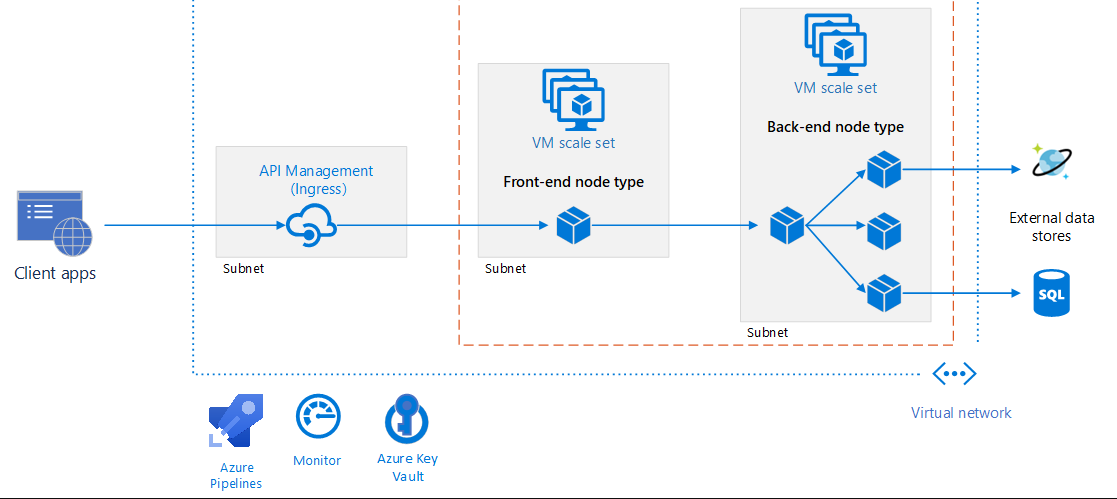
\includegraphics[width=1\linewidth]{images/design/front-back.png}
    \caption{FrontEnd + Backend \cite{frontbackazure}}
\end{figure}

Pero, no solo de esto se nutre la arquitectura del sistema, ya que, también tendriamos que incluir el proceso de Integración Continua / Distribución Continua (Continuous Integration and Continuous Delivery, CI/CD \cite{cicd}) que se encarga de los despliegues automatizados para evitar esa pesada, repetitiva y tortuosa carga.

El CI/CD que hemos utilizado para hacer los despliegues automatizados no es más que el por defecto que tiene la plataforma GitHub. Hemos utilizado este y no Azure Pipeline debido a que lo ideal es que el mismo sistema de repositorio sea el encargado de construir la aplicación y desplegarla en la cloud, y que no sea Azure el encargado de dicha tarea. Esto es debido a que, si el dia de mañana decidimos cambiar, solo tendriamos que cambiar parte de la arquitectura o servicios que se usan, pero no el CI/CD.

A continuación, en la Figura 5.2 se muestra de forma breve y sencilla todo el proceso.

\begin{figure}[H]
    \centering
    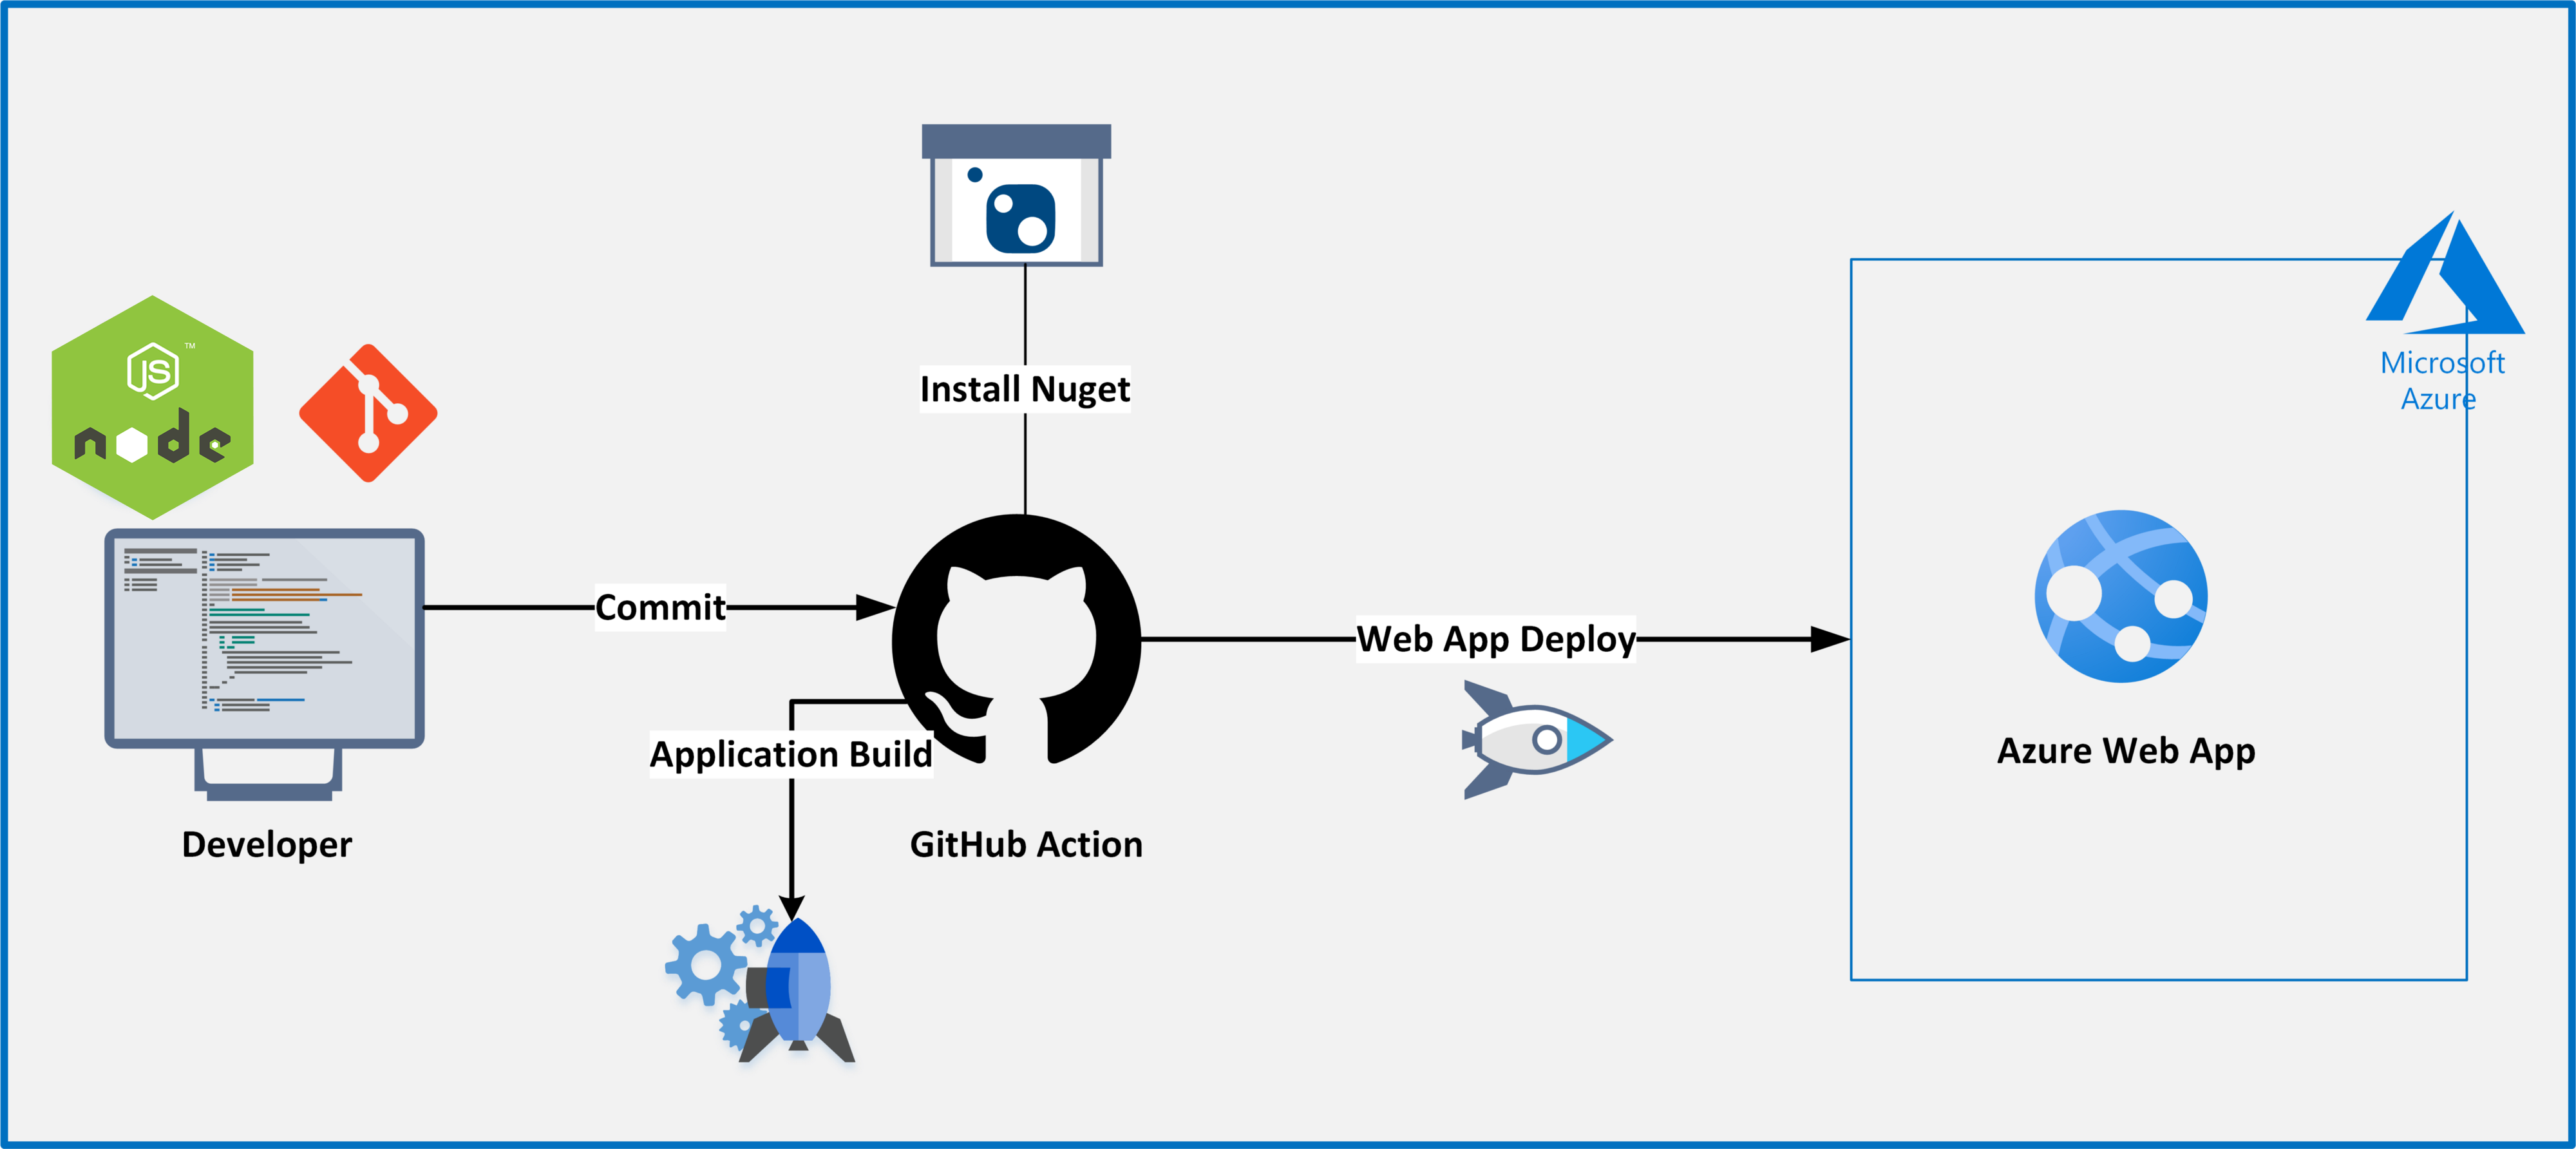
\includegraphics[width=1\linewidth]{images/design/github azure.png}
    \caption{GitHub Workflow Action + Azure \cite{github-azure}}
\end{figure}

\subsection{Sistema de IoT}
Por otra parte, el Sistema de IoT tiene su propia arquitectura, ya que, aunque comparte plataforma, Azure Cloud, el despliegue, el funcionamiento y el mismo concepto persé cambian drásticamente al de un sistema distribuido puro del tipo backend más frontend.

Este sistema tiene una arquitectura típica de todos los sistemas de IoT, es decir, dispositivo creador de eventos simples, un procesador de patrones de eventos simples y que si el patrón coincide, dispara el evento complejo y por último, un dispositivo que este atento a los eventos complejos y ejecute la acción por defecto que tengan asignada.

A continuación, exponemos en la Figura 5.3 como y que componentes tiene este sistema de IoT con Azure Cloud.

\begin{figure}[H]
    \centering
    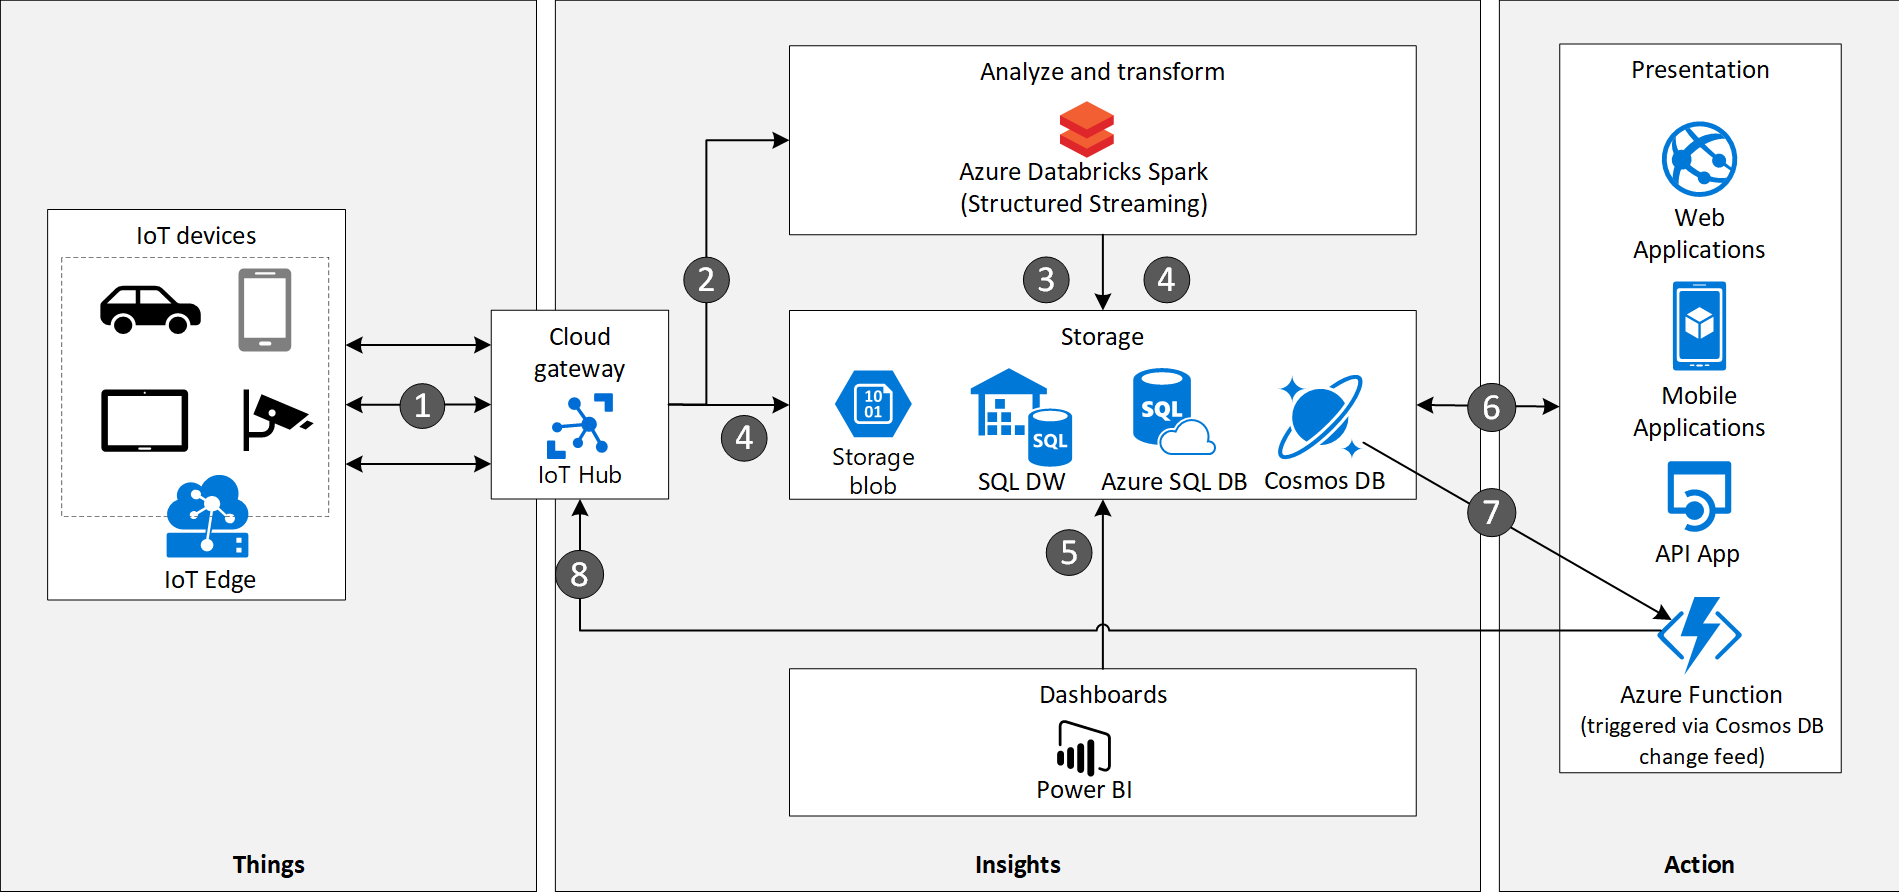
\includegraphics[width=1\linewidth]{images/design/iot-using-cosmos-db.png}
    \caption{IoT Azure \cite{iot-azure}}
\end{figure}

\section{Modelo Relacional}
En este apartado, exponemos el modelo relacional de la base de datos, es decir, que tablas posee y la relación entre las mismas. Además, mostramos las tablas y las relaciones que tienen entre sí, en las Figuras 5.4, 5.5, 5.6 y 5.7.

\begin{figure}[H]
    \centering
    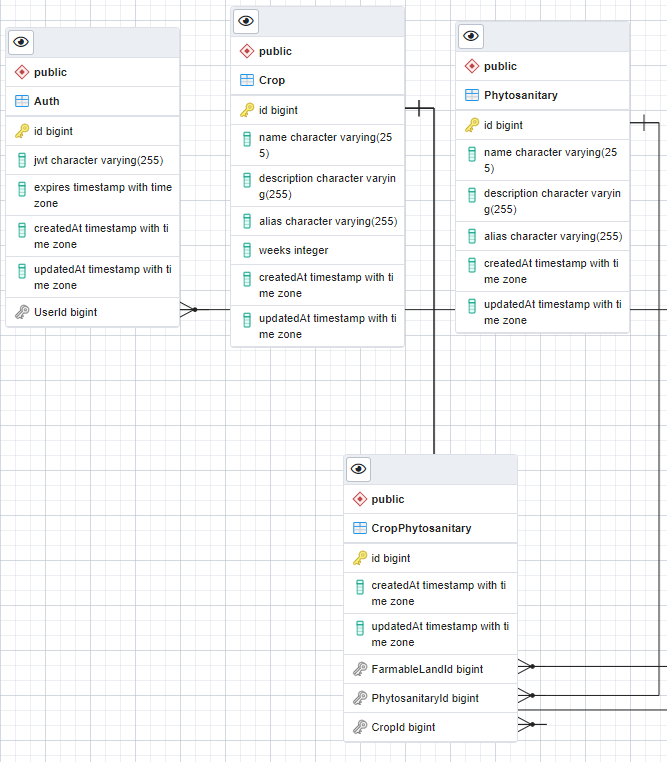
\includegraphics[width=1\linewidth]{images/design/erd1.png}
    \caption{Tablas Auth, Crop, Phytosanitary y CropPhytosanitary}
\end{figure}

\begin{figure}[H]
    \centering
    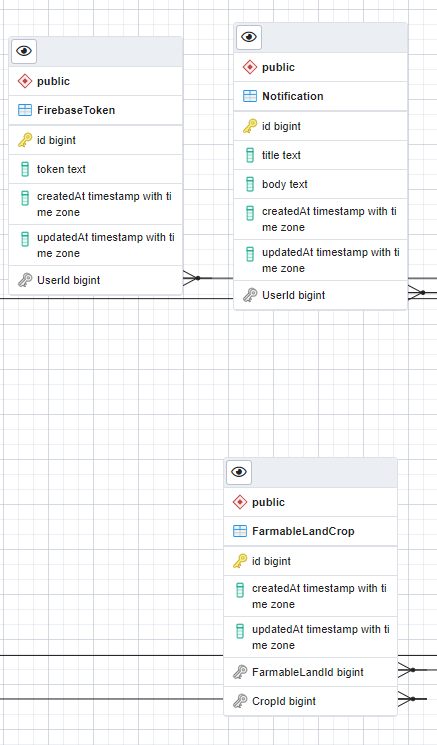
\includegraphics[width=1\linewidth]{images/design/erd2.png}
    \caption{Tablas FrebaseToken, Notification y FarmableLandCrop}
\end{figure}

\begin{figure}[H]
    \centering
    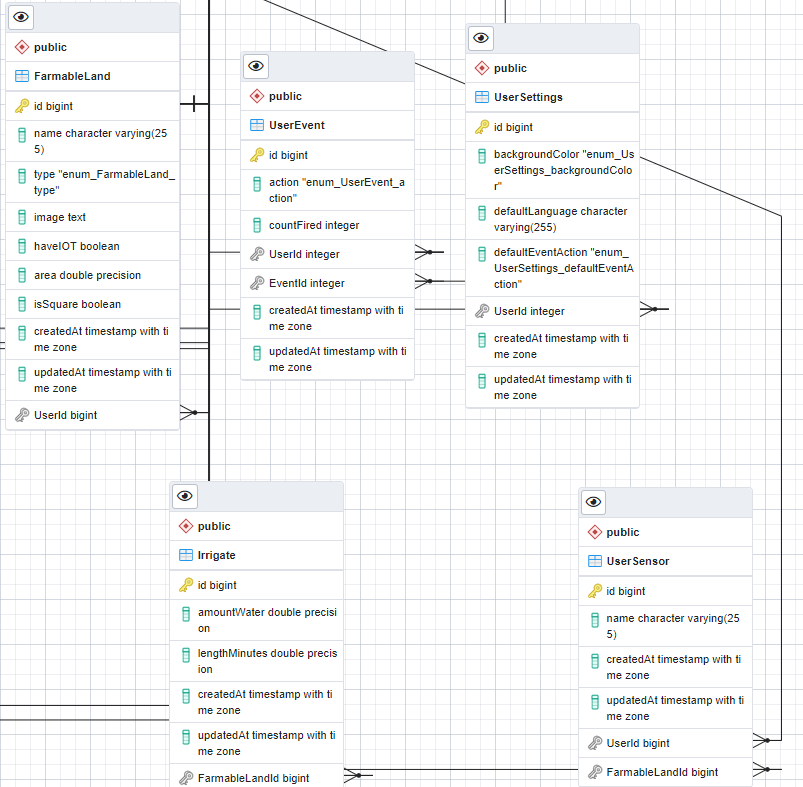
\includegraphics[width=1\linewidth]{images/design/erd3.png}
    \caption{Tablas FarmableLand, UserEvent, UserSettings, Irrigate y UserSensor}
\end{figure}

\begin{figure}[H]
    \centering
    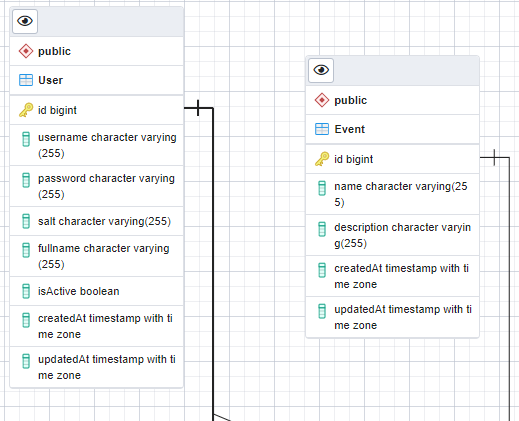
\includegraphics[width=1\linewidth]{images/design/erd4.png}
    \caption{Tablas User y Event}
\end{figure}

Además, para aclarar la composición de las tablas, listamos a continuación las mismas con sus columnas y con una breve descripción.

\begin{itemize}
    \item Auth: tabla dedicada a almacenar la información de autenticación del usuario.
    \item Crop: tabla dedicada a almacenar la información de los cultivos.
    \item Phytosanitary: tabla dedicada a almacenar la información de los fitosanitarios.
    \item CropPhytosanitary: tabla dedicada a relacionar los cultivos con los fitosanitarios.
    \item FirebaseToken: tabla dedicada a almacenar el token de dispositivo generado por firebase.
    \item Notification: tabla dedicada a almacenar las notificaciones del usuario.
    \item FarmableLandCrop: tabla dedicada a relacionar los terrenos con los cultivos.
    \item FarmableLand: tabla dedicada a almacenar los terrenos.
    \item UserEvent: tabla dedicada a relacionar los eventos complejos con un usuario.
    \item UserSettings: tabla dedicada a almacenar los ajustes del sistema del usuario.
    \item Irrigate: tabla dedicada a almacenar los riegos de los terrenos.
    \item UserSensor: tabla dedicada a relacionar sensores con usuarios.
    \item User: tabla dedicada a almacenar los usuarios del sistema.
    \item Event: tabla dedicada a almacenar los eventos complejos disponibles.
\end{itemize}

\section{Diseño de la interfaz}
Para el diseño de la interfaz, se ha usado una guía de diseño minimalista, donde predominan los espacios abiertos y con poca carga visual. Es decir, interfaz sencilla y que permita al usuario saber de un vistazo donde esta todo.

Por otra parte, como nuestro público objetivo son personas del mundo rural, se ha simplificado aún más ciertas tareas como las búsquedas, donde no se han puesto filtros ni elementos añadidos que puedan abrumar al usuario.

Además, la paleta de colores ha sido importante, ya que, uniamos las acciones peligrosas y sin vuelta atrás con el rojo, mientras que a las acciones informativas o de actualizan con capacidad de retorno, con colores más amenos como azul o verde. Todo ello, siempre en tonos claros, ya que, como se dijo anteriormente, la predominancia del color es el blanco y con colores claros no hay mucho contraste que pueda impactar de forma negativa al usuario.

Las imágenes, aunque siempre coloridas, se les ha impuesto en todos los casos un tamaño máximo para que no descuadre todos los componentes de su entorno, fácilitando así al usuario el seguir encontrado todo en su sitio y sin tener que volver a investigar donde esta todo de nuevo.

También, un elemento importante es el texto. Como siempre, hemos intentado que sean textos minimalistas, que con muy poco texto describa la situación o componente. De hecho, la parte de la aplicación que tiene más texto son las notificaciones que se envían al usuario cuando se dispara algún evento complejo.

Por último, para los componentes meramente visuales, se han usado los componentes del SDK Ionic \cite{ui-ionic}.
    \chapter{Implementación}
    En este capítulo se expondrán las distintas tecnologías usadas para el desarrollo del proyecto así como el repositorio en GitHub donde se encuentra almacenado el código fuente del proyecto.

\newpage

\section{Base de Datos}
Aquí expondremos el tipo de base de datos utilizado, así los métodos usados para desplegarlo tanto en local como en remoto.

\subsection{PostgreSQL}
La base de datos que se ha utilizado para este proyecto es PostgreSQL \cite{postgresql}. Hemos elegido este Sistema Gestor de Base de Datos (SGBD) debido a su gran versátilidad y debido a que continene una cantidad de caracteristicas que otras base de datos como MySQL \cite{mysql} o MariaDB \cite{mariadb} no tienen.

Además, su integración con el ORM (Object Relational Mapping) Sequelize \cite{sequelize} es prácticamente total, dando Sequelize soporte casi a la mayoría de las caracteristicas que te permite el SGBD PostgreSQL.

\subsection{Docker}
Para desplegar la base de datos, hemos usado una imagen Docker, para así evitar usar una instalación en local con una versión en concreto y arriesgarnos que con futuras actualizaciones de los sistemas operativos subyacentes den problemas.

A continuación, exponemos el código del docker-compose.yml en el Listado 6.1.

\begin{lstlisting}[language=XML,caption={docker-compose.yml},captionpos=b]
version: '3'
services:
  postgresql:
    image: postgres:9.6
    volumes:
      - smartrural:/var/lib/postgresql/data
    ports:
      - 5432:5432
    environment:
      - POSTGRES_DB=smartrural
      - POSTGRES_USER=smartrural
      - POSTGRES_PASSWORD=smartrural
volumes:
  smartrural:
    external: false
\end{lstlisting}

\subsection{Relational Database Service}
Por último, respecto a la base de datos, para tener una base de datos remota que pueda usar el software cuando se instala en el dominio remoto, hemos usado el servicio de Amazon Web Services (AWS) llamado Relational Database Service (RDS).

Debido a cuestiones económicas, hemos decidido optar por esta implementación de AWS en vez de usar la base de datos de Azure. Así que, al ser este un sistema puramente distribuido, da igual donde se aloje la base de datos. Mientras que se pueda acceder a ella de forma pública con una conexión de internet, es un servicio perfectamente válido.

A continuación, en la Figura 6.1 se puede apreciar la base de datos en el portal web de AWS.

\begin{figure}[H]
    \centering
    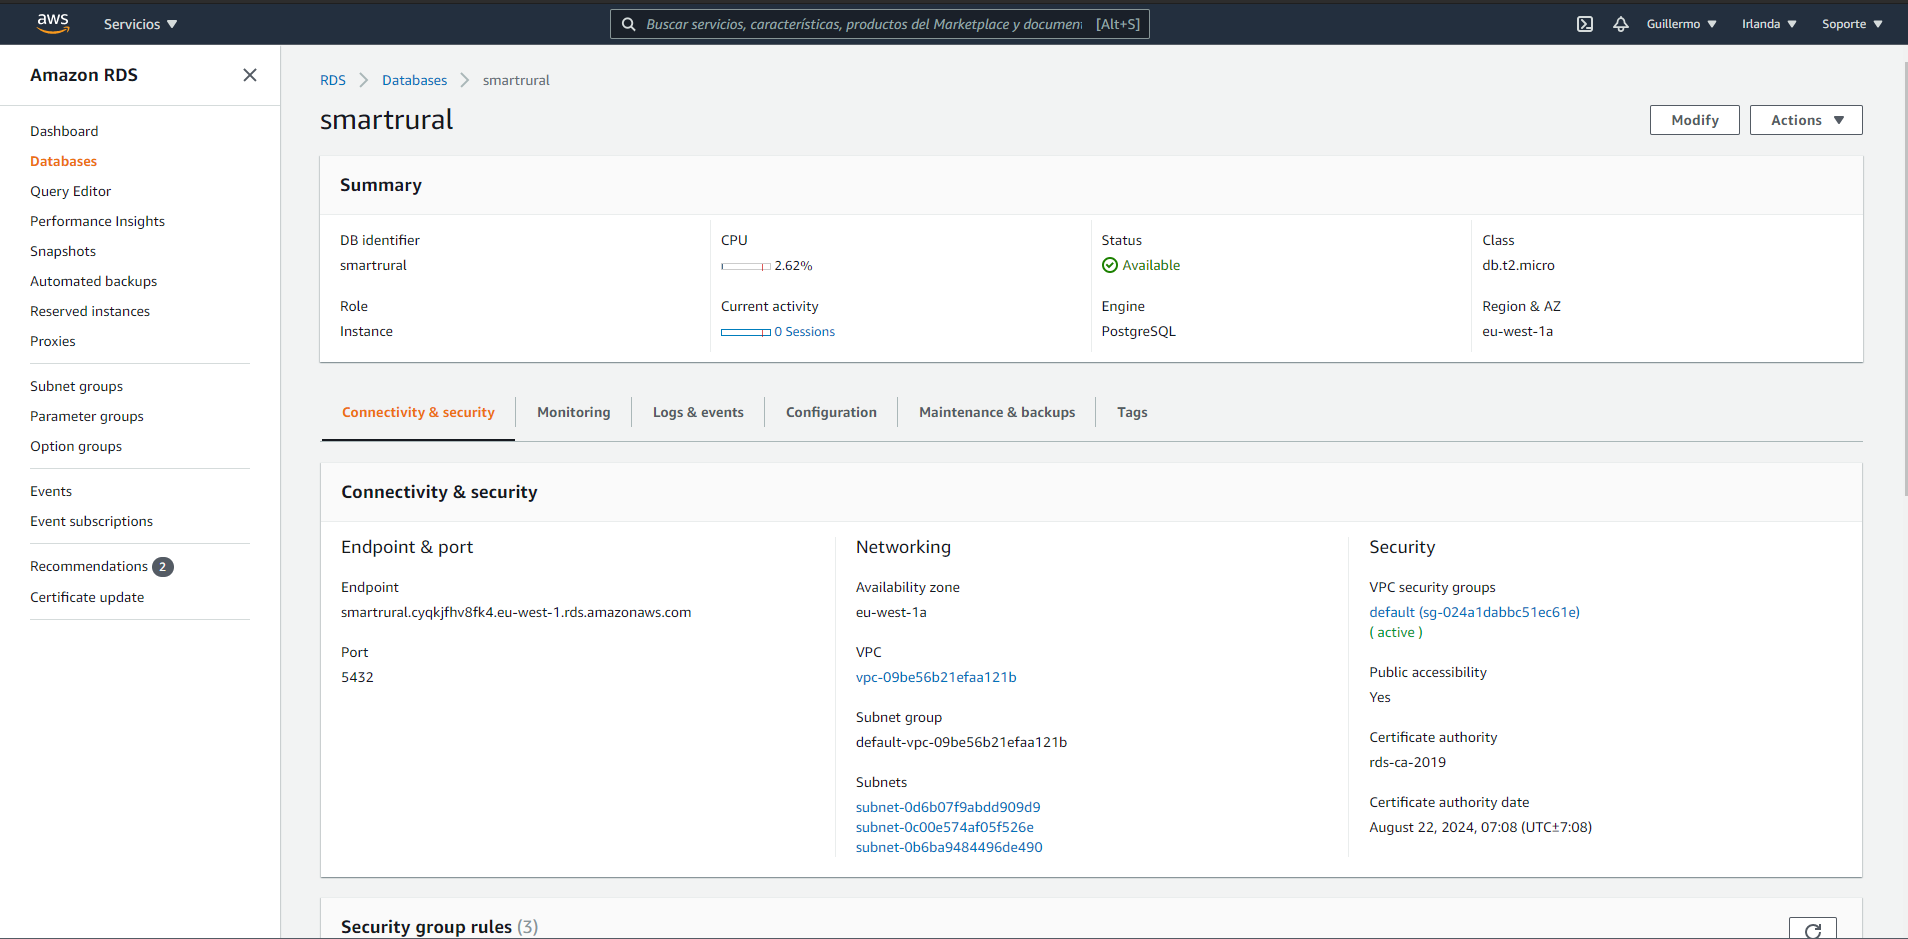
\includegraphics[width=1\linewidth]{images/implementation/database/aws rds.png}
    \caption{AWS RDS PostgreSQL}
\end{figure}

\section{Backend}
Aquí expondremos las distintas partes que conforman el backend y como se relacionan entre sí.

\subsection{Modelo de datos}
Para facilitar el uso de la base de datos y hacer un Create Read Update Delete (CRUD) en sus tablas, se ha usado un ORM y el concepto de modelo de datos, para crear entidades vivientes en lugar de operaciones sobre tablas de base de datos.

Los modelos usados son:

\begin{itemize}
    \item Auth: modelo usado para almacenar el token de sesión del login del usuario.
    \item Crop: modelo usado para almacenar los cultivos.
    \item CropPhytosanitary: modelo usado para relacionar un cultivo con un fitosanitario.
    \item Event: modelo usado para almacenar los eventos complejos a los que suscribirse.
    \item FarmableLand: modelo para almacenar los terrenos de un usuario.
    \item FarmableLandCrop: modelo para relacionar los terrrenos con un cultivo.
    \item FirebaseToken: modelo para almacenar los token de las notificaciones push de un usuario.
    \item Irrigate: modelo para almacenar los riegos de un terreno.
    \item Notification: modelo para almacenar las notificaciones de un usuario.
    \item Phytosanitary: modelo para almacenar los fitosanitarios.
    \item User: modelo para almacenar los usuarios.
    \item UserEvent: modelo para relacionar a un usuario con una serie de eventos complejos.
    \item UserSensor: modelo para relacionar a una serie de sensores con un usuario.
    \item UserSettings: modelo para almacenar los ajustes del sistema de un usuario.
\end{itemize}

Estos modelos han sido declarados todos en archivos con formato de tipo JavaScript (JS).

A continuación, exponemos en la Figura 6.2 la ruta de donde se declaran los modelos y en el Listado 6.2 la declaración de un modelo en código fuente.

\begin{figure}[H]
    \centering
    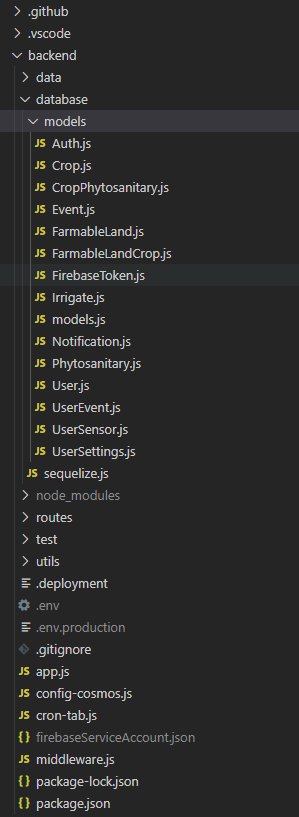
\includegraphics[width=0.4\linewidth]{images/implementation/backend/backend models.png}
    \caption{Estructura del Backend con los modelos}
\end{figure}

\begin{lstlisting}[language=Java,caption={Declaración de modelo},captionpos=b]
const { Model, DataTypes } = require('sequelize');

const sequelize = require('../sequelize');
const User = require('./User');

class Auth extends Model {}

Auth.init({
  id: {
    type: DataTypes.BIGINT,
    autoIncrement: true,
    primaryKey: true
  },
  jwt: {
    type: DataTypes.STRING
  },
  expires: {
    type: DataTypes.DATE
  }
}, {
  sequelize,
  modelName: 'Auth',
  freezeTableName: true,
  tableName: 'Auth',
  timestamps: true,
});

Auth.prototype.isValid = function() {
  return (
    new Date(this.expires).getTime() >= new Date().getTime()
  );
}

Auth.belongsTo(User);

module.exports = Auth;
\end{lstlisting}

\subsection{Sequelize}
Para trasladar los modelos anteriormente descritos a tablas de base de datos con sus columnas y demás propiedades, se ha usado el ORM Sequelize. Este ORM es sumamente versátil y muy completo, y en caso de que el día de mañana se quisiera cambiar de SGBD, solo tendríamos que cambiar el tipo del dialecto a usar.

Así pues, tan solo con un reinicio del Backend, podriamos pasar de usar una base de datos en PostgreSQL a una en MySQL, SQL Server, SQLite o cualquier otra típico SGBD del mercado.

A continuación, en el Listado 6.3 se muestra como se instancia Sequelize con los valores predeterminados.

\begin{lstlisting}[language=Java,caption={Creación de instancia de Sequelize},captionpos=b]
const { Sequelize } = require('sequelize');

let dialectOptions = {};
if(process.env.ENVIRONMENT === 'production')
{
  dialectOptions = {
    ssl: {
      require: true,
      rejectUnauthorized: false
    }
  }
}

const sequelize = new Sequelize(
  process.env.DATABASE_NAME,
  process.env.DATABASE_USERNAME,
  process.env.DATABASE_PASSWORD,
  {
    host: process.env.DATABASE_HOST,
    dialect: process.env.DATABASE_DIALECT,
    dialectOptions: dialectOptions,
    logging: (process.env.ENVIRONMENT === 'production'),
  }
);

module.exports = sequelize;
\end{lstlisting}

\subsection{Servicios}
Para mejorar la modularización de todo el backend y que de forma efectiva se pueda cambiar la lógica cuando se necesite, hemos creado una capa de servicios.

Dichos servicios son llamados desde de los controladores y desde de los servicios de creación de base de datos con datos de ejemplo.

Además, estos servicios también son usados en los test, por lo cual, si más adelante se cambia la lógica de los servicios, mientras se mantenga la precondición y la postcondición, los test seguirán funcionando.

A continuación, en el Listado 6.4, exponemos el servicio de envio de creación de usuarios como ejemplo de servicio.

\begin{lstlisting}[language=Java,caption={Servicio de Creación de Usuario},captionpos=b]
const User = require('../../database/models/User');
const { setPassword } = require('../../utils/password');

const createUser = async(username, password, fullname) => {
  const { hash, salt } = setPassword(password);
  return await User.create({
    username: username,
    password: hash,
    salt: salt,
    fullname: fullname,
    isActive: true
  });
};

module.exports = {
  createUser
};
\end{lstlisting}

\subsection{Middleware}
Uno de los aspectos más importantes para nuestro backend es la seguridad. Y para ello, tenemos que establecer un sistema de login seguro, fiable y fácilmente resoluble.

Este sistema de login, se comprueba mediante este middleware. Cada vez que se accede a un endpoint distinto al de login, se comprueba que el token de sesión existe y es veraz. Si no lo es, al pasar por ese middleware, el endpoint automáticamente dara un error con el código 401 Unauthorized.

A continuación, exponemos en el Listado 6.5 la codificación del middleware que se usa en la totalidad de los endpoints \cite{endpoint}.

\begin{lstlisting}[language=Java,caption={Middleware},captionpos=b]
const Auth = require('./database/models/Auth');
const User = require('./database/models/User');
const { Op } = require('sequelize');
const { verifyToken } = require('./utils/jwt');

const middleware = async (req, res, next) => {
  try
  {
    const token = (req.headers['authorization'] !== null) ? req.headers['authorization'].split(' ')[1] : null;
    if (token)
    {
      const auth = await Auth.findOne({
        where: {
          jwt: token,
          expires: {
            [Op.gt]: new Date()
          }
        }
      });

      if(auth && auth.isValid())
      {
        const user = await User.findOne({
          where: {
            id: auth.UserId
          }
        });
        const verify = verifyToken(user.username, user.salt, token);

        if(verify)
        {
          req.username = user.username;
          next();
        } else
        {
          throw new Error('token cannot be verified');
        }
      } else
      {
        throw new Error('token invalid');
      }
    } else
    {
      throw new Error('token not send');
    }
  } catch(err)
  {
    res.status(401).send({
    msg: (Object.keys(err).length === 0) ? 'token not send' : err
    });
  }
}

const unless = (paths, middleware) => {
  return (req, res, next) => {
  // res.setHeader('Access-Control-Allow-Origin', '*');
  // res.setHeader('Access-Control-Allow-Methods', 'GET, POST, OPTIONS, PUT, PATCH, DELETE');
  for (const path of paths)
  {
    if(path.path === req.path && path.method === req.method)
    return next();
  }
  return middleware(req, res, next);
  };
};

module.exports = {
  middleware, unless
};
\end{lstlisting}

\subsection{Testing}
Para garantizar que algunas funcionalidades funcionan despues de modificar cualquier parte del código y que cumplen todos los requisitos que deben tener, se ha creado una parte de testing.

En concreto, son test unitarios y de integración, donde se comprueba el funcionamiento unitario de servicios y su integración con los controladores.

A continuación, exponemos en el Listado 6.6 un fragmento de los test creados para comprobar la funcionalidad de creación de un usuario.

\begin{lstlisting}[language=Java,caption={Test User},captionpos=b]
const axios = require('axios').default;

process.env.ENVFILE = '.env';
const dotenv = require('dotenv');
dotenv.config({ path: process.env.ENVFILE });

const { createUser } = require('../routes/services/create-user');
const { removeUser } = require('../routes/services/remove-user');

const timeout = 1000000;
const baseURL = 'http://localhost:3000/api/v1';
const localServer = axios.create({
  baseURL: baseURL,
  timeout: timeout,
});

const testUser = {
  username: 'testing',
  password: 'testing',
  fullname: 'Guillermo Lopez Garcia'
};

describe('create user', function() {
  it('create correct user', async () => {
    const user = await createUser(
      testUser.username,
      testUser.password,
      testUser.fullname
    );
  }).timeout(timeout);

  it('login correct user', async () => {
    const login = (await localServer.post('/login', {
      username: testUser.username,
      password: testUser.password,
    })).data;
  }).timeout(timeout);

  it('get correct user', async () => {
    const login = (await localServer.post('/login', {
      username: testUser.username,
      password: testUser.password,
    })).data;

    const localServerAuth = axios.create({
      baseURL: baseURL,
      timeout: timeout,
      headers: { 'Authorization': 'Bearer ' + login.token }
    });

    const user = (await localServerAuth.get('/user/fullname', {
      params: {
        username: testUser.fullname
      }
    })).data;
  }).timeout(timeout);

  it('destroy correct user', async () => {
    const confirm = await removeUser(testUser.username);
  }).timeout(timeout);
});
\end{lstlisting}

\subsection{Notificaciones}
Para poder realizar las notificaciones al usuario cuando un evento complejo se dispara, nos hemos visto obligado a realizar este componente del Backend.

Esta parte, no es más que un crontab \cite{crontab} que se nutre de servicios que acceden a Azure CosmosDB \cite{cosmosdb} y que está consultado cada breve intervalo de tiempo consulta la base de datos NoSQL de CosmosDB por si hubiera algún evento complejo que se hubiera disparado.

A continuación, exponemos en los Listados 6.7 y 6.8 el servicio para obtener los datos de Azure CosmosDB \cite{cosmosdb} y como enviar notificaciones a los dispositivos con firebase \cite{firebase}.

\begin{lstlisting}[language=Java,caption={Listado de Eventos de Azure CosmosDB},captionpos=b]
const CosmosClient = require("@azure/cosmos").CosmosClient;

const { config } = require('../../config-cosmos');
const { endpoint, key, databaseId, containerId } = config;

const client = new CosmosClient({ endpoint, key });

const database = client.database(databaseId);
const container = database.container(containerId);

const getAllEventFromCosmos = async () => {
  const querySpec = {
    query: `SELECT * FROM c`
  };
  const { resources: items } = await container.items.query(querySpec).fetchAll();
  return items;
}

const removeEventsFromCosmos = async (items = []) => {
  for(const item of items)
  {
    const { id, sensorId } = item;
    const { resource: result } = await container.item(id, sensorId).delete();
  }
}

const getEventFromCosmos = async (sensorId) => {
  const querySpec = {
    query: `SELECT * FROM c WHERE c.sensorId = '${sensorId}'`
  };
  const { resources: items } = await container.items.query(querySpec).fetchAll();
  return items;
}

module.exports = {
  getEventFromCosmos, getAllEventFromCosmos, removeEventsFromCosmos
};
\end{lstlisting}

\begin{lstlisting}[language=Java,caption={Enviar notificación a dispositivo},captionpos=b]
const admin = require('firebase-admin');
const serviceAccount = require('../../firebaseServiceAccount.json');
admin.initializeApp({
  credential: admin.credential.cert(serviceAccount)
});

const FirebaseToken = require('../../database/models/FirebaseToken');

const sendNotificationToUser = async (userId, notification) => {
  const firebaseTokens = await FirebaseToken.findAll({
    where: {
      UserId: userId
    }
  });

  let responses = [];
  for(const firebaseToken of firebaseTokens)
  {
    // This registration token comes from the client FCM SDKs.
    const registrationToken = firebaseToken.token;

    const message = {
      notification: notification
    };

    responses.push(
      await admin.messaging().sendToDevice(registrationToken, message, {
        priority: "high",
        timeToLive: 60 * 60 * 24
      })
    );
  }

  return responses;
};

module.exports = { sendNotificationToUser };
\end{lstlisting}

\subsection{Environment}
Para poder parametrizar correctamente el acceso a servicios externos, como base de datos o credenciales para firebase, se han creado ficheros que guarden dichas credenciales y mediante la bibliteca DotEnv, se incluyen en la variables de entorno de NodeJS.

A continuación, exponemos los Listados 6.9, 6.10 y 6.11 de dichos ficheros de credenciales donde se han omitido algunos valores para no comprometer la seguridad de dichos servicios en ningún momento.

\begin{lstlisting}[language=Java,caption={Fichero .env},captionpos=b]
DATABASE_NAME=smartrural
DATABASE_USERNAME=smartrural
DATABASE_PASSWORD=smartrural
DATABASE_HOST=127.0.0.1
DATABASE_DIALECT=postgres
ENVIRONMENT=develop

COSMOS_ENDPOINT=
COSMOS_KEY=
COSMOS_DATABASE=
COSMOS_CONTAINER_ID=
\end{lstlisting}

\begin{lstlisting}[language=Java,caption={Fichero .env.production},captionpos=b]
DATABASE_NAME=smartrural
DATABASE_USERNAME=smartrural
DATABASE_PASSWORD=
DATABASE_HOST=smartrural.cyqkjfhv8fk4.eu-west-1.rds.amazonaws.com
DATABASE_DIALECT=postgres
ENVIRONMENT=production

COSMOS_ENDPOINT=
COSMOS_KEY=
COSMOS_DATABASE=
COSMOS_CONTAINER_ID=
\end{lstlisting}

\begin{lstlisting}[language=Java,caption={Fichero firebaseServiceAccount.json},captionpos=b]
{
  "type": "service_account",
  "project_id": "",
  "private_key_id": "",
  "private_key": "",
  "client_email": "",
  "client_id": "",
  "auth_uri": "",
  "token_uri": "",
  "auth_provider_x509_cert_url": "",
  "client_x509_cert_url": ""
}
\end{lstlisting}

\subsection{App}
Por último respecto al Backend, tenemos la creación de la instancia del servidor a través de una IP y un puerto, donde en local siempre será la dirección IP de bucle local, 127.0.0.1, y el puerto 3000. En remoto, ocupará el puerto 80 con el dominio \textcolor{blue}{\href{https://backend-tfg.azurewebsites.net}{https://backend-tfg.azurewebsites.net}}.

A través de la creación del Backend, se instancia servicios como el crontab para los servicios complejos o el propio sequelize para acceder a la base de datos.

A continuación, mostramos el código que se encarga de iniciar nuestro Backend en el Listado 6.12.

\begin{lstlisting}[language=Java,caption={App.js},captionpos=b]
const express = require('express');
const app = express();
const logger = require('morgan');
const http = require('http');
const PORT = process.env.PORT || 3000;
const bodyParser = require('body-parser');
const baseAPI = '/api/v1';
const cors = require('cors');

const args = process.argv.slice(2);
process.env.ENVFILE = (args[0]) ? args[0] : '.env';

const dotenv = require('dotenv');
dotenv.config({ path: process.env.ENVFILE });

app.use(cors({
  origin: '*'
}));
app.use(bodyParser.json({
  limit: '1024mb'
}));
app.use(logger('dev'));
app.use(bodyParser.urlencoded({
  extended: true,
  limit: '1024mb'
}));

const routes = require('./routes/routes');

for (const route of routes) {
  app.use(baseAPI, route);
}

const sequelize = require('./database/sequelize');

(async () => {
  await sequelize.sync();
})();

const { initCronTab } = require('./cron-tab');
initCronTab();

const server = http.createServer(app);
server.listen(PORT, function() {
    console.log('Server up and running on localhost:' + PORT);
});
\end{lstlisting}

\section{Frontend}
Aquí expondremos las distintas partes que conforman el frontend y como se relacionan entre sí.

\subsection{Componentes}
Para hacer una correcta modularización del Frontend y no hacer repeticiones en el código, se han creado una serie de componentes, una unidad modular de un programa software con interfaces y dependencias bien definidas, que se reutilizan a lo largo del proyecto. Los componentes creados son:

\begin{itemize}
    \item Menu: componente creado para hacer el menú.
    \item Refresher: componente creado para hacer la funcionalidad del refresher, es decir, refrescar la página con nueva información.
    \item Toolbar: componente creado para establecer un header común a todas las páginas, para así establecer los iconoes que desee de forma fácil con la típica barra de búsqueda.
\end{itemize}

A continuación, exponemos la Figura 6.3 para mostrar de forma visual dichos componentes en el directorio del proyecto.

\begin{figure}[H]
    \centering
    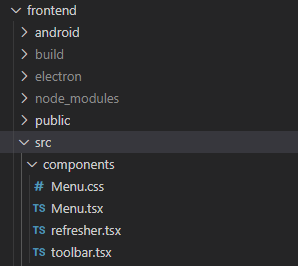
\includegraphics[width=0.7\linewidth]{images/implementation/frontend/frontend components.png}
    \caption{Componentes}
\end{figure}

\subsection{Páginas}
Como todo Frontend que se precie, debe tener distintas páginas, para así favorecer la correcta modularización de las funcionalidades.

Las páginas creadas son:
\begin{itemize}
    \item Home: página creada para ver de un vistazo todas las secciones de la aplicación.
    \item Crop: páginas creadas para hacer el CRUD sobre los cultivos.
    \item Events: páginas creadas para realizar la suscripción a los eventos complejos.
    \item FarmableLand: páginas creadas para hacer el CRUD sobre los terrenos.
    \item Irrigate: páginas creadas para hacer el CRUD sobre los riegos de los terrenos.
    \item Login: página creada para permitir el acceso correcto al sistema mediante la introducción correcta de las credenciales de usuario, formada por nombre de usuario y contraseña.
    \item Notifications: página creada para ver por orden de más cercano a más lejano en el tiempo todas las notificaciones al usuario.
    \item Phytosanitary: páginas creadas para hacer el CRUD sobre los fitosanitarios de los cultivos.
    \item Settings: página creada para ver y modificar los ajustes del sistema del usuario, tales como aspecto visual, idioma por defecto y acción por defecto en los eventos complejos.
\end{itemize}

\subsection{Servicios}
Para poder reutilizar código, hemos creado una capa de servicio formado principalmente por funciones útiles reutilizables para los principales comportamientos que se repiten a lo largo de la aplicación frontal, tales como obtener la información de sesión - ajustes o bien, acceder a los endpoints con el correspondiente token de sesión.

También se usan funciones para el sistema traducción, i18n \cite{i18n} \cite{i18n-react}, y para el sistema de push notificacions de Firebase \cite{firebase}.

\subsection{Routes}
Para poder usar características como ``ir hacia atrás'', hemos necesitado diseñar un sistema de routes usando como base el sistema que nos da React.

A partir de aquí, mediante URL, podemos acceder a cualquiera de las páginas en caso de usar la aplicación. En caso de la aplicación móvil, internamente también se usan las URLs, pero como se traslada a un sistema de vistas como en Android nativo, así que funciona igual pero sin acceso a escribir la URL que se desee.

\subsection{Environment}
Para establecer las variables de entorno como en el Backend, se necesita también crear archivos de la extensión .env.

En concreto, para React, reconoce dos tipos de perfiles. El de ejecución local con livereload y el de production donde se realiza el build. Así pues, en principio tenemos dos ficheros de variables de entorno, .env y .env.production.

Pero a parte, como nosotros construimos la aplicación móvil Android, pues hemos agregado un tercer fichero de variables de entorno llamado .env.android para probar ejecuciones en local. Cuando la aplicación se construya para un modo de producción como la plataforma Google Play Store, pues se usará el fichero .env.production.

Por último, antes de exponer las imágenes de los ficheros, queda aclarar que para que una tecnología como React lea las variables de entorno, dichas variables tienen que empezar por el prefijo REACT\_APP\_.

A continuación, exponemos los 3 ficheros de variables de entorno con sus respectivos valores en los Listados 6.13, 6.14 y 6.15.

\begin{lstlisting}[language=Java,caption={Fichero .env},captionpos=b]
REACT_APP_BACKEND_HOST=http://localhost:3000
REACT_APP_CHECK_SESSION_TIME=1000000
\end{lstlisting}

\begin{lstlisting}[language=Java,caption={Fichero .env.production},captionpos=b]
REACT_APP_BACKEND_HOST=https://backend-tfg.azurewebsites.net
REACT_APP_CHECK_SESSION_TIME=1000000
\end{lstlisting}

\begin{lstlisting}[language=Java,caption={Fichero .env.android},captionpos=b]
REACT_APP_BACKEND_HOST=http://10.0.2.2:3000
REACT_APP_CHECK_SESSION_TIME=1000000
\end{lstlisting}

\subsection{App}
Respecto a la creación de la instancia de la aplicación frontal, no tiene mucha variación respecto a una instancia de una aplicación frontal con React, salvo por la pecurialidad de nuestro proyecto donde además es imperativo instanciar a su vez un servicio de Firebase para las notificaciones.

\subsection{Android}
Para la aplicación Android, hemos usado el SDK de Ionic para poder construir con el comando \textbf{ionic capacitor build android}.
Pero, no es lo único que se necesita hacer para que la aplicación Android funcione, ya que, tiene su propia complejidad activar las Push Notifications y permitir el uso de internet en la aplicación Android.

A continuación, exponemos en los Listados 6.16 y 6.17 las líneas de código añadidas a los ficheros para que funcione todo correctamente.

\begin{lstlisting}[language=Java,caption={Fichero app/build.gradle},captionpos=b]
dependencies {
    implementation platform('com.google.firebase:firebase-bom:27.1.0')
    implementation 'com.google.firebase:firebase-analytics'
}
\end{lstlisting}

\begin{lstlisting}[language=XML,caption={Fichero AndroidManifest.xml},captionpos=b]
...
    <application
        android:allowBackup="true"
        android:icon="@mipmap/ic_launcher"
        android:label="@string/app_name"
        android:roundIcon="@mipmap/ic_launcher_round"
        android:supportsRtl="true"
        android:theme="@style/AppTheme"
        android:usesCleartextTraffic="true">
...
\end{lstlisting}

\subsection{Web}
Para la aplicación más usada como es la aplicación web del Frontend, solo tiene un particularidad con respecto al código base, y es que para que el servicio de notificaciones funcione, se necesita a parte un ``Service Worker'' para estar leyendo dichas notificaciones y mostrarlas en el frontal.

Para ejecutar la aplicación web, se puede usar el comando \textbf{ionic serve}.

\subsection{Desktop}
Por último, respecto a la aplicación frontal, existe la aplicación de escritorio. Esta aplicación se construye con el SDK de Ionic con el comando \textbf{ionic capacitor build electron}

\section{Sistema IoT}
Aquí expondremos las distintas partes que conforman el Sistema de IoT y como se relacionan entre sí.

\subsection{Emulator}
Como todo Sistema de IoT, tiene una parte de creación de eventos simples. En concreto, esto en nuestro proyecto se hace con la creación de un dispositivo virtual que simula dichos eventos simples.

\subsection{Stream Analytics}
Otra parte fundamental de un Sistema de IoT es la parte de los patrones.

Esto en nuestro proyecto se realiza con el servicio de Stream Analytics de Azure Cloud \cite{stream-analytics}, el cual tiene su propio lenguaje y características.

Como ejemplo de codificación del patrón de eventos simples, exponemos en el Listado 6.18 nuestro patrón o consulta para detectar el evento complejo ``Irrigate''.

\begin{lstlisting}[language=SQL,caption={ASASmartRural-Irrigate.asaql},captionpos=b]
SELECT
  sensorId AS sensorId,
  'Irrigate' AS EventFired,
  COUNT(*) AS count
INTO
  [CosmosDB]
FROM
  [IoTHub]
WHERE
  isAtDaytime = 1
  and
  isRaining = 0
  and
  airHumidity < 30
  and
  roomTemperature < 25
GROUP BY
  sensorId, TumblingWindow(minute, 1)
\end{lstlisting}

\subsection{Azure CosmosDB}
Por último, una parte que no puede faltar en un Sistema de IoT es la del postprocesamiento del evento complejo. Es decir, una vez que se ha disparado ese evento complejo, se debe realizar una acción.

Esta acción en un nuestro proyecto es almacenar dicho evento complejo en una base de datos NoSQL como es Azure CosmosDB. Esta base de datos actua como ``stage'' intermediario temporal, donde cada cierto periodo de tiempo, el Backend acudé a dicha base de datos, obtiene los eventos complejos lanzados y actúa en consecuencia.

Por supuesto, una vez que obtiene los datos, limpia la base de datos para que no surja repetición de los mismos.

A continuación, exponemos en la Figura 6.4 un ejemplo del tipo de datos que se almacena en la base de datos de Azure CosmosDB.

\begin{figure}[H]
    \centering
    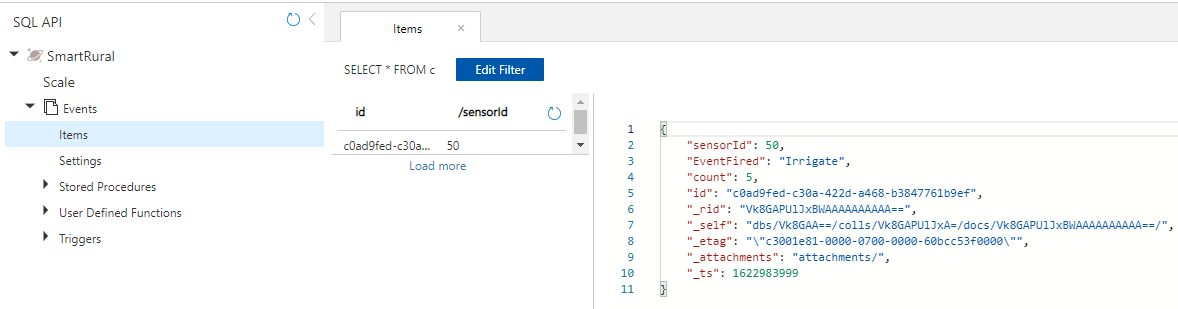
\includegraphics[width=1\linewidth]{images/implementation/iot/iot cosmosdb object.png}
    \caption{Azure CosmosDB Object}
\end{figure}
    \chapter{Pruebas}
    En este capítulo se mostrarán las distintas tipologías de pruebas que existen como introducción a las mismas y las que se han realizado tanto en el Backend como en el Frontend para verificar la funcionalidad del sistema añadiendo así calidad a nuestro proyecto.

\newpage

El testing, como concepto general, se basa en investigaciones y técnicas que se encargan de proporcionar información sobre el producto software y de si este cumple con todas las condiciones de calidad para ser llevado a un sistema de producción o de cliente final.

A su vez, como existen distintos tipos de software, existen distintos tipos de pruebas. A continuación, listamos los tipos más genéricos y damos una breve descripción de para que sirven.

\begin{itemize}
    \item Pruebas unitarias: se basa en comprobar la veracidad o funcionamiento correcto de un trozo de código, generalmente una función o método de un objeto.
    \item Pruebas de integración: se realizan siempre a posteriori de las pruebas unitarias y se basa justamente en probar en conjunto lo probado en las pruebas unitarias para comprobar que la integración de esas funcionalidades no da ningún error.
    \item Pruebas de humo: son pruebas rápidas, generalmente manuales, que se encarga de comprobar el flujo principal del software y algunos casos secundarios, pero sin profundizar en ellos.
    \item Pruebas alpha: son pruebas que se hacen durante el desarrollo del software y se encargan de verificar que el producto software que se está desarrollando, es útil y válido para el cliente.
    \item Pruebas beta: son pruebas que se hacen cuando el desarrollo está terminado y se hacen en un entorno semireal o de semiproducción.
    \item Pruebas de aceptación: estas pruebas se realizan cuando la generación de la release del producto software está próxima y se encarga de verificar que se cumplen todos los requisitos funcionales. Se alternan pruebas automáticas y manuales.
    \item Pruebas de regresión: estas pruebas se basan en buscar errores, en lugar de buscar una correcta ejecución del software. Son bastantes últiles a la hora de detectar situaciones limite no contempladas anteriormente.
    \item Pruebas de compatibilidad: se basa en probar el sistema de distintos entorno para comprobar su correcto funcionamiento. Esto no es más que, ejecutar el software en distintos sistemas operativos para ver que ocurre.
    \item Pruebas de usabilidad: estas pruebas suelen ser manuales y se basan en que los distintos usuarios para lo que está orientado el producto software interactúen con dicho programa y detecten las carencias que tenga en materia de usar el propio software.
    \item Pruebas de rendimiento: estas pruebas se basan en ejecutar el software en distintas máquinas con variedad de recursos hardware para ver como se comporta. Si el software solo puede ejecutarse con una especificación hardware en concreto, no se considera de inmediato que el software este mal, si no que eso hay que contrastarlo con las especificaciones hardware del sistema de producción.
    \item Pruebas de escalabilidad: estas pruebas suelene ser automáticas y se basan en aplicar distinta carga de datos de entrada al software y ver como es capaz de escalar según la demanda y sus recursos software asignados. Este tipo de pruebas esta íntimamente ligadas con las pruebas de carga.
\end{itemize}

Pero, según el software, se aplican unas pruebas u otras. En el contexto de los sistemas distribuidos, se puede dividir en 2 grupos:

\begin{itemize}
    \item Pruebas funcionales: son pruebas de caja negra que se centra en que dada una precondición, se cumple una postcondición en un tiempo determinado. Su función principal es comprobar si el producto tiene la calidad suficiente para entrar en producción.
    \item Pruebas no funcionales: son pruebas dedicadas a comprobar detalles que no estén intimamente ligados con el uso final del software.
\end{itemize}

Así pues, pasaremos a definir que tipos de test se han realizado en los 2 bloques principales.

\section{Backend}
En el Backend, las principales pruebas han sido manuales. La única prueba automática se ha realizado ha sido la concerniente a la creación, login y eliminación de un usuario.

Es decir, se ha hecho una prueba automátizada para probar todo el ciclo de vida de un usuario.

Esta prueba se ha realizado de forma automatizada, ya que, prueba uno de los aspectos más importantes de la aplicación. Es decir, la seguridad de acceso al sistema.

Esta prueba ha sido realizada con MochaJS \cite{mochajs}.

Por lo demás, se ha probado todo de forma manual e integrado con el Frontend. El motivo de no haber hecho más pruebas automatizadas ha sido el tiempo y la no necesidad de ser exhaustivo en este aspecto con un proyecto de esta magnitud.

A continuación, en la Figura 7.1, se muestra el resultado de los test en el Backend.

\begin{figure}[H]
    \centering
    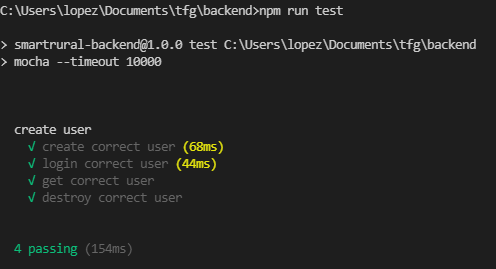
\includegraphics[width=0.7\linewidth]{images/test/test user backend.png}
    \caption{npm run test}
\end{figure}

\section{Frontend}
En el Frontend, todas las pruebas realizadas han sido manuales integradas con el Backend. La única prueba realizada de forma automática ha sido una prueba generica donde se comprueba que la aplicación base se renderiza de forma correcta. Esta prueba ha sido realizada con Jest \cite{jest}. En la Figura 7.2 se muestra el resultado de los tests.

\begin{figure}[H]
    \centering
    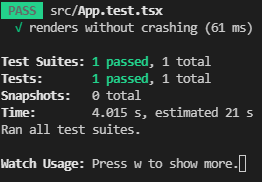
\includegraphics[width=0.7\linewidth]{images/test/test app frontend.png}
    \caption{npm run test}
\end{figure}

Por lo demás, todo ha sido probado con distintas pruebas manuales en integración con el Backend, a la hora de comprobar si obtenia la información de forma correcta y rápida.

    \chapter{Conclusiones}
    Respecto a este último capítulo, mostraremos todo lo que se ha aprendido con este proyecto y el trabajo futuro del mismo.

\newpage

\section{Ámbito}
Respecto al ámbito, las conclusiones obtenidas han sido muy beneficiosas. Hemos conseguido con éxito elaborar una aplicación multiplataforma que permite al usuario gestionar todos sus recursos rurales e integra a la perfección con todas las nuevas tecnologías que actualmente imperan en el mercado.

\section{Aprendizaje}
Con este proyecto hemos aprendido como es el funcionamiento de una de las Cloud Públicas más relevantes en la actualidad, es decir, Azure Cloud.

Además, respecto al Backend, se ha aprendido a crear desde cero un sistema de login fiable y seguro, mediante un token de sesión. A parte, de diversos conocimientos adquiridos a la hora de conectar desde local con los servicios de Azure Cloud y como operar con dichos servicios dentro de operaciones de cron-tab.

Por otra parte, en el Frontend, se ha aprendido una tecnología que ahora mismo es una de las más importantes a saber del sector, como es React. Además, se ha aprendido usando la nueva forma de componentes funcionales, es decir, es lugar de crear objetos de clases, usando funciones.

Además, se ha aprendido respecto a usar el CI/CD que ofrece GitHub con su GitHub Workflow Action y como sincronizarlo con Azure para optimizar al máximo los despliegues. Como añadido, se ha usado esto que ofrece GitHub para además hacer compilaciones automáticas de esta documentación para mayor facilidad a la hora de obtenerla de forma sencilla para su entregable.

También, se ha aprendido a usar todo el soporte que ofrece Azure Cloud para un Sistema de IoT, Internet of Things, el cual es bastante completo.

\section{Problemas encontrados}
Los problemas encontrados han sido diversos.

El más destacado ha sido el precio de los servicios usados. Azure, como es normal, ofrece un buen servicio pero no a costo cero. Entonces, el desembolso que se ha tenido que hacer para poder usar la Cloud ha sido destacable.

Otro de los problemas encontrados, ha sido la integración de Stream Analytics con Azure CosmosDB, ya que, si se quería insertar información desde el primero al segundo, hacia falta hacer configuraciones un tanto complejas de las cuales apenas había información.

Por último, uno de los mayores problemas encontrados ha sido integrar Firebase de Google Cloud Platform con el Frontend para poder acceder a las Push Notifications tanto desde la plataforma web como desde el móvil.

Hemos de destacar que todos estos problemas se resolviero con éxito, pero han tomado bastante tiempo y horas dedicadas a la investigación de la documentación de por medio.

\section{Trabajo Futuro}
Por último, el presente proyecto tiene bastantes características deseables, pero le faltan algunas que, para un proyecto empresarial, serían sumamente imprescindibles.

Estas características son:

\begin{itemize}
    \item Mayor accesibilidad. Esta característica es sumamente importante, sobre todo cuando se trata de llegar al mayor número de clientes potenciales posibles. Uno de los principales elementos a implementar sería un sistema de TalkBack o Lector de Pantalla \cite{talkback}.
    \item Apartado de ayuda. Esta característica, como su propia nombre indica, se basaría en implementar un sistema de ayuda, incluso con un pequeño chat para ayudar al usuario a resolver dudas sobre el uso de la aplicación.
    \item Generar en Google Play Store y en Apple Store una aplicación del proyecto. Esta característica se implementaría únicamente para facilitar la descarga y la instalación de la aplicación en los dispositivos móviles de los usuarios.
    \item Crear más test tanto en Backend como en Frontend. Esta característica se implementaría usando las tecnologías de test de cada parte del proyecto y su beneficio sería aumentar la calidad y facilitar la comprobación de que el software funciona como debería en cada parte del mismo.
    \item Crear un BackOffice para un administrador total. Esta característica se implementaría en un Frontend a parte del usuario habitual. El principal beneficio sería el de diferenciar un administrador normal del administrador total que controla los recursos directamente en la nube.
    \item Cambiar el dispositivo que envía los eventos simples de un simulador a un dispositivo real, es decir, sensor más Raspberry Pi.
    \item Mejorar el CI/CD añadiendo la construcción y publicación de las aplicaciones móviles. Esta características se implementaría usando GitHub Workflow y el beneficio sería inmediato, es decir, eliminar al programador la engorrosa tarea de construir la aplicación y subirla posteriormente a la Play Store o a la App Store.
\end{itemize}

    \begin{thebibliography}{9}
    \bibitem{backend} Backend Concept, \url{https://developer.mozilla.org/es/docs/Learn/Server-side/First_steps/Introduction}. Último acceso: 16/06/2021 16:29:00.
    \bibitem{frontend} Frontend Concept, \url{https://developer.mozilla.org/es/docs/Learn/Front-end_web_developer}. Último acceso: 16/06/2021 16:29:00.
    \bibitem{nodejs} NodeJS, \url{https://nodejs.org/es/}. Último acceso: 16/06/2021 16:29:00.
    \bibitem{ionic} Ionic, \url{https://ionicframework.com/}. Último acceso: 16/06/2021 16:29:00.
    \bibitem{react} React, \url{https://es.reactjs.org/}. Último acceso: 16/06/2021 16:29:00.
    \bibitem{azure} Azure, \url{https://azure.microsoft.com/es-es/}. Último acceso: 16/06/2021 16:29:00.
    \bibitem{smart-village} Smart Village, \url{https://enrd.ec.europa.eu/smart-and-competitive-rural-areas/smart-villages/smart-villages-portal_es}. Último acceso: 16/06/2021 16:29:00.
    \bibitem{e40group} E40 Group, \url{https://www.e40.eu/}. Último acceso: 16/06/2021 16:29:00.
    \bibitem{ifls} Ifls, \url{https://www.ifls.com.co/que-es-ifls/}. Último acceso: 16/06/2021 16:29:00.
    \bibitem{innovatiesteunput} Innovatiesteunput, \url{https://www.innovatiesteunpunt.be/nl/wedstrijdregelement-innovatiecampagne-2020}. Último acceso: 16/06/2021 16:29:00.
    \bibitem{greece} Agricultural University of Athens, \url{https://www2.aua.gr/en}. Último acceso: 16/06/2021 16:29:00.
    \bibitem{econcepts} eConcepts, \url{https://www.econcepts.ie/}. Último acceso: 16/06/2021 16:29:00.
    \bibitem{smart-rural} Smart Rural, \url{https://smartrural.net/}. Último acceso: 16/06/2021 16:29:00.
    \bibitem{team-smartrural} Equipo y Premios Smart Rural, \url{https://smartrural.net/empresa-de-agricultura-inteligente/#equipo-smartrural}. Último acceso: 16/06/2021 16:29:00.
    \bibitem{scrum} Scrum Definition, \url{https://es.wikipedia.org/wiki/Scrum_(desarrollo_de_software)}. Último acceso: 16/06/2021 16:29:00.
    \bibitem{cleancode} Clean Code Wikipedia, \url{https://es.wikipedia.org/wiki/Robert_C._Martin}. Último acceso: 16/06/2021 16:29:00.
    \bibitem{cleancodebook} Clean Code Book, \url{https://www.amazon.es/Clean-Code-Handbook-Software-Craftsmanship/dp/0132350882/}. Último acceso: 16/06/2021 16:29:00.
    \bibitem{iso25010} ISO 25010, \url{https://iso25000.com/index.php/normas-iso-25000/iso-25010}. Último acceso: 16/06/2021 16:29:00.
    \bibitem{cicd} CI/CD Explicación Castellano RedHat, \url{https://www.redhat.com/es/topics/devops/what-is-ci-cd}. Último acceso: 16/06/2021 16:29:00.
    \bibitem{endpoint} Endpoint o Punto final de comunicación, \url{https://es.wikipedia.org/wiki/Punto_final_de_comunicaci\%C3\%B3n}. Último acceso: 16/06/2021 16:29:00.
    \bibitem{ui-ionic} UI Components Ionic, \url{https://ionicframework.com/docs/components}. Último acceso: 16/06/2021 16:29:00.
    \bibitem{postgresql} PostgreSQL, \url{https://www.postgresql.org/}. Último acceso: 16/06/2021 16:29:00.
    \bibitem{mysql} MySQL, \url{https://www.mysql.com/}. Último acceso: 16/06/2021 16:29:00.
    \bibitem{mariadb} MariaDB, \url{https://mariadb.org/}. Último acceso: 16/06/2021 16:29:00.
    \bibitem{sequelize} Sequelize, \url{http://sequelize.org/}. Último acceso: 16/06/2021 16:29:00.
    \bibitem{crontab} crontab, \url{https://es.wikipedia.org/wiki/Cron_(Unix)}. Último acceso: 16/06/2021 16:29:00.
    \bibitem{cosmosdb} Azure CosmosDB, \url{https://azure.microsoft.com/es-es/services/cosmos-db/}. Último acceso: 16/06/2021 16:29:00.
    \bibitem{dotenv} DotEnv Library, \url{https://www.npmjs.com/package/dotenv}. Último acceso: 16/06/2021 16:29:00.
    \bibitem{i18n} i18n, \url{https://developer.mozilla.org/es/docs/Mozilla/Add-ons/WebExtensions/API/i18n}. Último acceso: 16/06/2021 16:29:00.
    \bibitem{i18n-react} i18n React, \url{https://react.i18next.com/}. Último acceso: 16/06/2021 16:29:00.
    \bibitem{firebase} Firebase, \url{https://firebase.google.com/docs}. Último acceso: 16/06/2021 16:29:00.
    \bibitem{stream-analytics} Stream Analytics, \url{https://docs.microsoft.com/es-es/stream-analytics-query/stream-analytics-query-language-reference}. Último acceso: 16/06/2021 16:29:00.
    \bibitem{mochajs} MochaJS, \url{https://mochajs.org/}. Último acceso: 16/06/2021 16:29:00.
    \bibitem{jest} React Jest, \url{https://jestjs.io/es-ES/}. Último acceso: 16/06/2021 16:29:00.
    \bibitem{talkback} Lector de Pantalla, \url{https://es.wikipedia.org/wiki/Lector_de_pantalla}. Último acceso: 16/06/2021 16:29:00.
    \bibitem{frontbackazure} Arquitectura Front Back Azure, \url{https://docs.microsoft.com/es-es/azure/architecture/reference-architectures/microservices/service-fabric}. Último acceso: 16/06/2021 16:29:00.
    \bibitem{github-azure} GitHub Workflow con Azure, \url{https://blog.bitsrc.io/using-github-actions-with-azure-app-services-for-web-apps-1d3333c391d4}. Último acceso: 16/06/2021 16:29:00.
    \bibitem{iot-azure} IoT Azure, \url{https://docs.microsoft.com/es-es/azure/architecture/solution-ideas/articles/iot-using-cosmos-db}. Último acceso: 16/06/2021 16:29:00.
\end{thebibliography}

    \chapter{Anexos}
    \section{Manual de Instalación}

En este capítulo hablaremos sobre la instalación de las tecnologías necesarias y con sus configuraciones para arrancar el proyecto de forma satisfactoria.

Además, las tecnologías seleccionadas suelen tener un gran grado de retrocompatibilidad, así que, aunque se podrán versiones en concreto, muy seguramente con versiones más nuevas el proyecto funcionará igual.

\newpage

\subsection{Git}
Para instalar Git, solo tenemos que seguir los pasos del siguiente enlace \textcolor{blue}{\href{https://git-scm.com/book/en/v2/Getting-Started-Installing-Git}{Git}}

\subsection{Docker}
Con este sistema de virtualización, nos permite instalar versiones antiguas de software, que muchas veces con las actualizaciones de los sistema operativos, sin imposibles de actualizar.

Sobre todo, lo que más importa con eso son las base de datos, ya que son los casos más evidentes y más comunes. Veasé con el caso de MySQL 5.8.

Así pues, siguiendo las instrucciones de \textcolor{blue}{\href{https://docs.docker.com/engine/install}{Docker}}, instalaremos Docker en nuestro sistema.

\subsection{PostgreSQL}
Para instanciar una base de datos de PostgreSQL, usaremos lo instalado en el paso anterior y simplmente levantaremos el fichero docker-compose.yml y ya tenemos la base de datos que necesitamos.

\subsection{NVM}
Otro de los sistemas que necesitamos es NodeJS. Pero en vez de instalarnos el binario tal cual, usaremos esta tecnología llamada Node Version Manager.

Para instalar dicha tecnología, seguiremos las siguientes instrucciones \textcolor{blue}{\href{https://github.com/nvm-sh/nvm}{NVM}}.

Por último, para instalar NodeJS junto con su versión de NPM, solo tendremos que ejecutar el comando \textbf{nvm install 14}. Esto instala la versión de NodeJS 14.x.

\subsection{Ionic}
A parte de NodeJS y NPM, necesitamos el SDK de Ionic.

Este SDK lo podemos instalar con NPM, ejecutando el siguiente comando \textbf{npm install -g @ionic/cli}

Una vez lo tengamos instalado, solo tendremos que realizar el comando \textbf{ionic -v} para verificar dicha instalación.

\subsection{Código fuente}
Para obtener el código fuente de la aplicación, solo tenemos que hacer un git clone del repositorio. Dicho repositorio, es el siguiente: \textcolor{blue}{\href{https://github.com/guilogar/tfg}{https://github.com/guilogar/tfg}}.

Por tanto, si queremos hacer el clone, ejecutariamos el comando \\
\textbf{git clone https://github.com/guilogar/tfg}.

\subsection{Backend}
Para terminar la instalación del Backend, solo tendriamos que crear los archivos de credenciales necesarios.

Para esto, solo hay que crear 2 ficheros. Uno con variables de entorno genericas para la ejecución local y otro para las credenciales de Firebase.

A continuación, expongo el formato de los mismos.

\begin{lstlisting}[language=Java,caption={Fichero .env},captionpos=b]
DATABASE_NAME=smartrural
DATABASE_USERNAME=smartrural
DATABASE_PASSWORD=smartrural
DATABASE_HOST=127.0.0.1
DATABASE_DIALECT=postgres
ENVIRONMENT=develop

COSMOS_ENDPOINT=...
COSMOS_KEY=...
COSMOS_DATABASE=...
COSMOS_CONTAINER_ID=...
\end{lstlisting}

\begin{lstlisting}[language=Java,caption={Fichero firebaseServiceAccount.json},captionpos=b]
{
  "type": "service_account",
  "project_id": "",
  "private_key_id": "",
  "private_key": "",
  "client_email": "",
  "client_id": "",
  "auth_uri": "",
  "token_uri": "",
  "auth_provider_x509_cert_url": "",
  "client_x509_cert_url": ""
}
\end{lstlisting}

Por último, para instanciar el Backend, tan solo son necesarios 4 comandos.

\begin{itemize}
    \item \textbf{docker-compose up -d}
    \item \textbf{cd backend}
    \item \textbf{npm install}
    \item \textbf{node .}
\end{itemize}

\subsection{Frontend}
Respecto al Frontend, los ficheros de variables de entorno están versionados. Por tanto, para iniciar el frontend solo necesita 3 comandos.

\begin{itemize}
    \item \textbf{cd frontend}
    \item \textbf{npm install}
    \item \textbf{ionic serve}
\end{itemize}

\subsection{Datos por defecto}
Para poder usar el proyecto en local, se necesitan datos por defecto. Para poder generarlos, ya existe una funcionalidad que se ha programado que lo hace de forma automática.

Para insertar estos datos de ejemplo, se puede usar el comando \textbf{npm run makeNewData}.

De estos datos de ejemplo, se inserta un usuario con las siguientes credenciales:

\begin{itemize}
    \item Username: \textbf{test}
    \item Password: \textbf{test}
\end{itemize}

\subsection{Emulator}
Respecto al simulador de eventos simples, también se necesita crear un archivo de variables de entorno. A continuación, exponemos el formato del mismo.

\begin{lstlisting}[language=Java,caption={Fichero emulator/.env},captionpos=b]
CONNECTION_STRING=...
TIME_INTERVAL=30000
\end{lstlisting}

Para ejecutar el simulador, solo hace falta 3 comandos.

\begin{itemize}
    \item \textbf{cd emulator}
    \item \textbf{npm install}
    \item \textbf{node .}
\end{itemize}
    \section{Manual de Usuario}
En este capítulo vamos a explicar como usar el software en cada uno de sus apartados.

\newpage

\subsection{Inicio de Sesión}
Para acceder a la aplicación, necesitamos pasar si o si por la pantalla de login. Esta pantalla es la primera que se ve en el primer acceso a la aplicación.

Para poder probar dicha aplicación de forma rápida, aconsejamos usar el usuario por defecto.
\begin{itemize}
    \item Username: \textbf{test}
    \item Password: \textbf{test}
\end{itemize}

\begin{figure}[H]
    \centering
    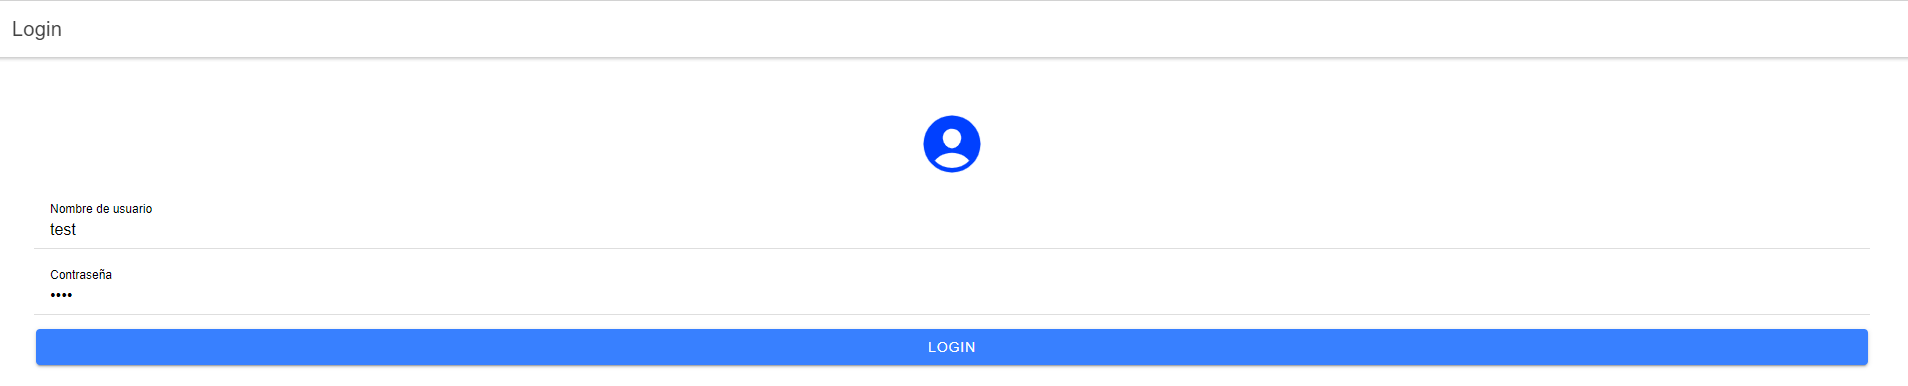
\includegraphics[width=1\linewidth]{images/user-manual/login.png}
    \caption{Inicio de Sesión}
\end{figure}

\subsection{Cerrar Sesión}
Para poder cerrar sesión, previamente se tiene que estar logeado y en el menú del dashboard. Una vez que se cumplen estas condiciones, es tan fácil como pulsar en la opción con el texto ``Cerrar sesión''.

\begin{figure}[H]
    \centering
    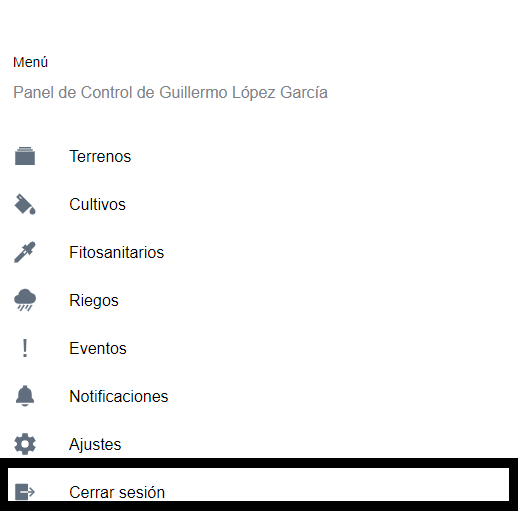
\includegraphics[width=0.7\linewidth]{images/user-manual/logout.png}
    \caption{Cerrar Sesión}
\end{figure}

\subsection{Dashboard}
Esta es la pantalla principal que ve el usuario cuando pasa el login. En esta pantalla, se puede ver el menú y todas las opciones que este tiene.

\begin{figure}[H]
    \centering
    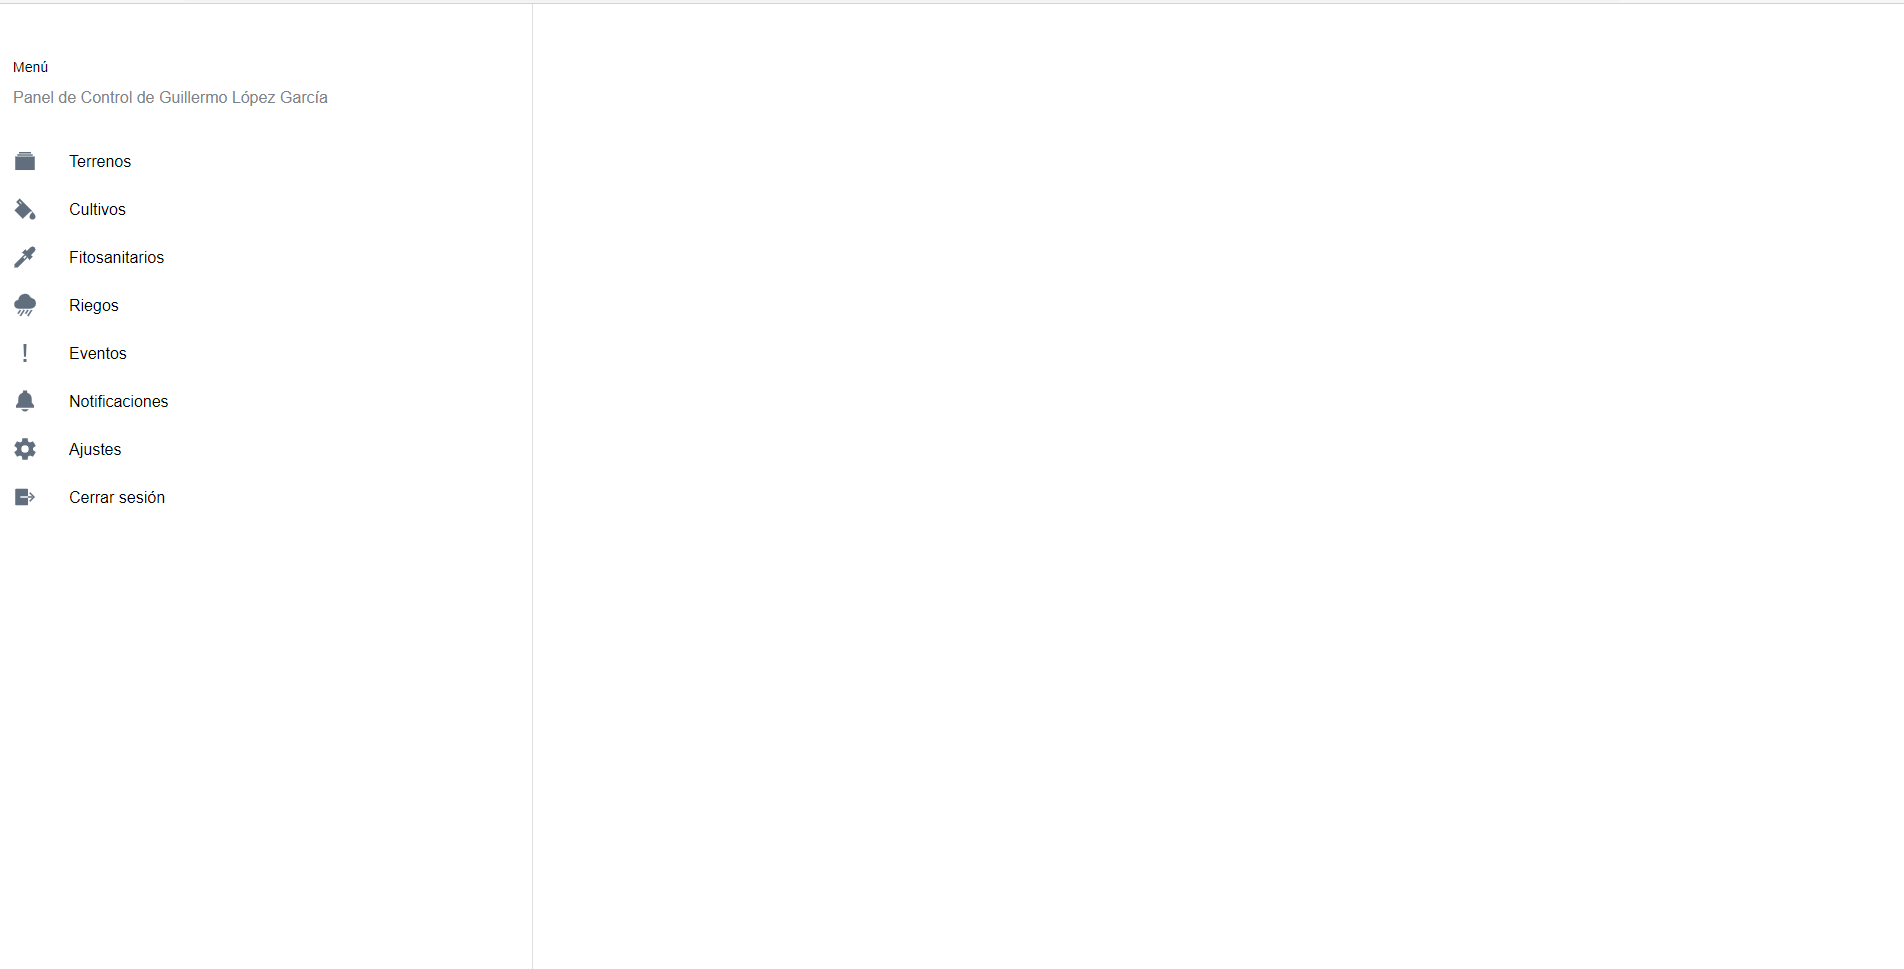
\includegraphics[width=0.7\linewidth]{images/user-manual/dashboard.png}
    \caption{Dashboard}
\end{figure}

\subsection{Inicio}
Esta pantalla, se convierte en la principal en caso de que se este usando la aplicación móvil o se este accediendo a la web desde un móvil.

Desde esta pantalla, se puede acceder a cualquiera de las secciones de la aplicación.

\begin{figure}[H]
    \centering
    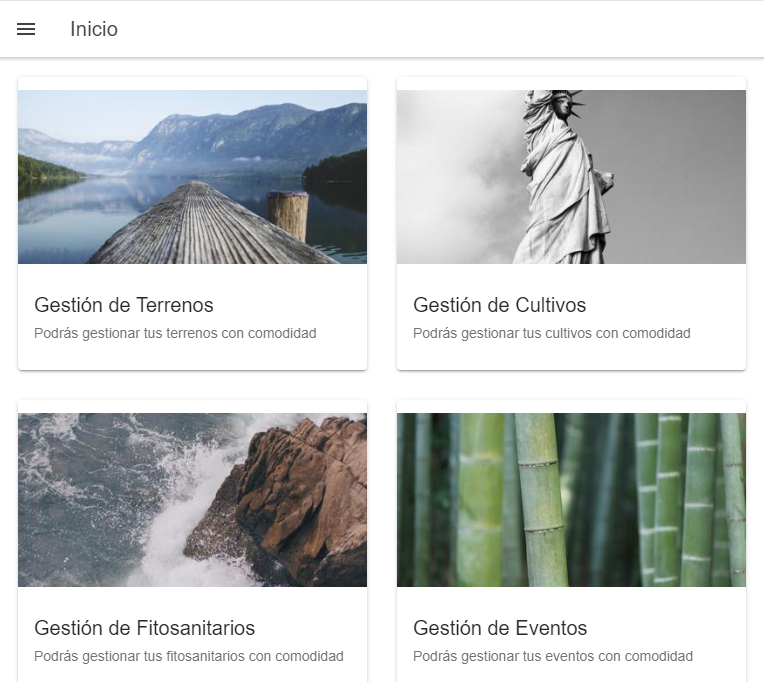
\includegraphics[width=0.7\linewidth]{images/user-manual/inicio.png}
    \caption{Inicio}
\end{figure}

\subsection{Terrenos}
En esta sección, se permite todo el CRUD de los terrenos. A continuación, se explica como se hace cada una de las operaciones.

\subsubsection{Listar}
Para listar los terrenos disponibles, tan solo tendremos que entrar en la sección de terrenos y de entrada los listará a todos, como se puede apreciar en la Figura 9.5.
\begin{figure}[H]
    \centering
    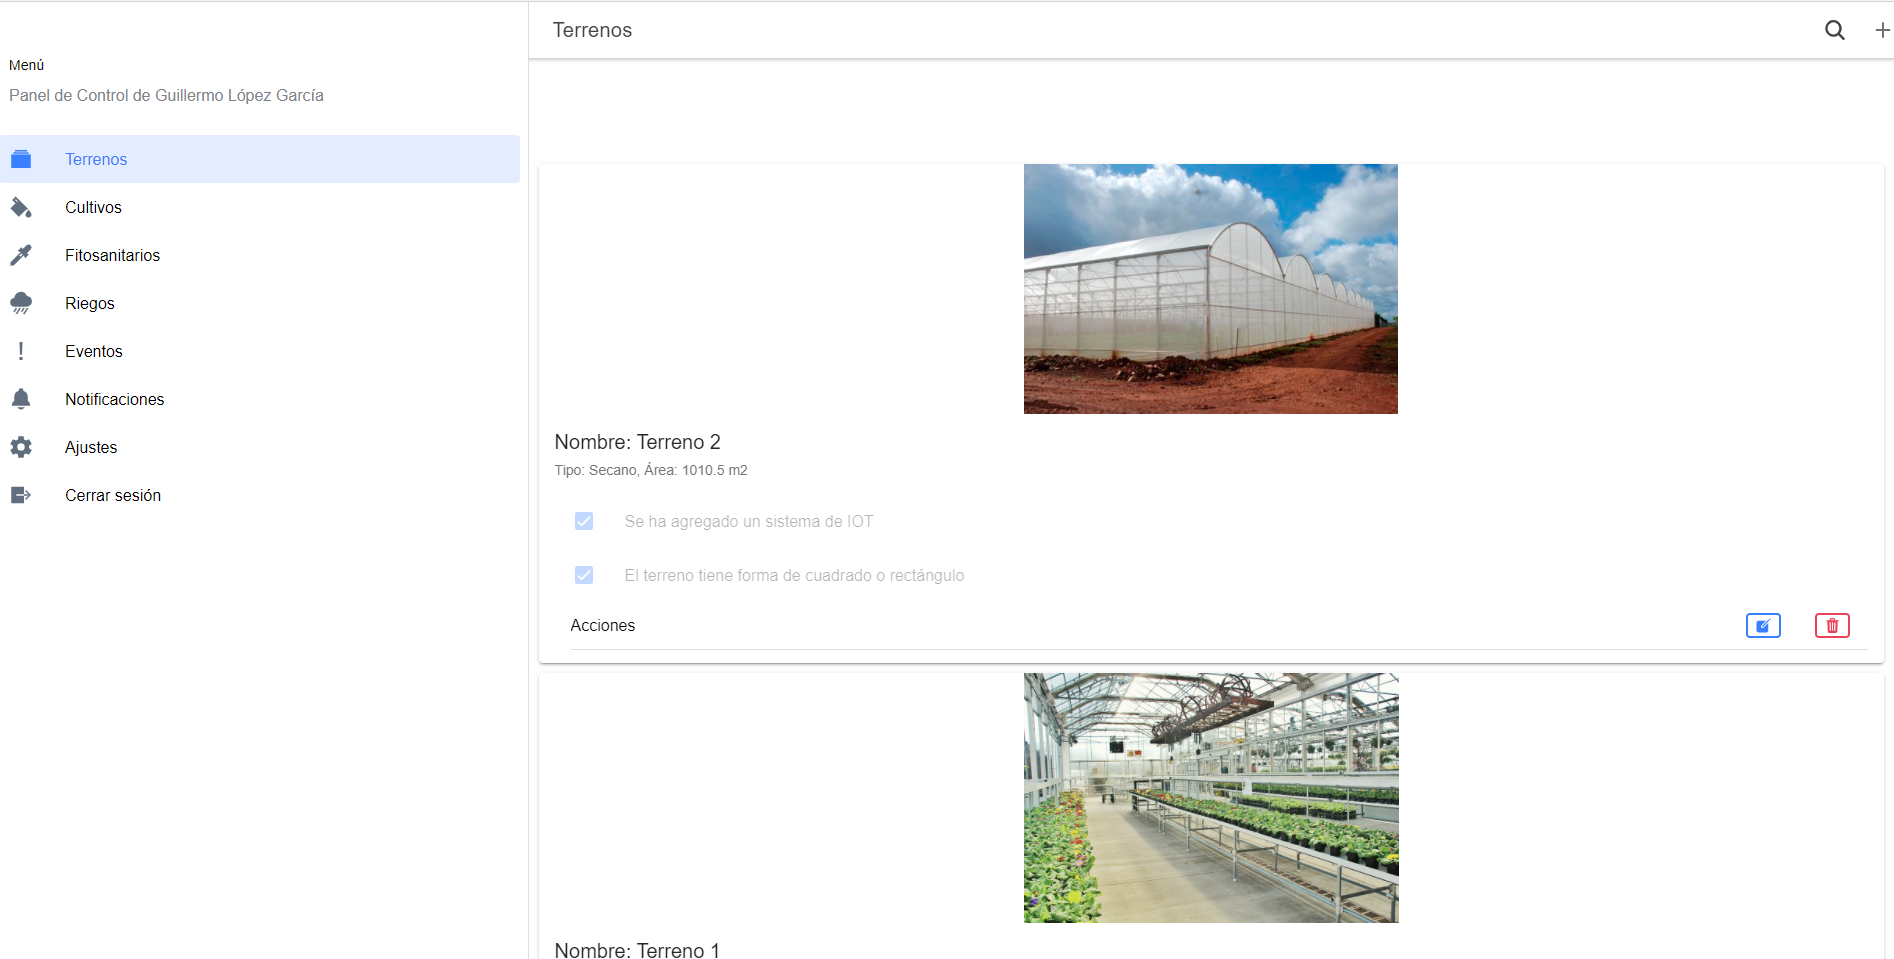
\includegraphics[width=0.7\linewidth]{images/user-manual/farmableland/list.png}
    \caption{Listar Terrenos}
\end{figure}

\subsubsection{Buscar}
Para buscar un terreno, el usuario debe pulsar en la barra superior que existe en la sección de terrenos y escribir la búsqueda deseada. A continuación, se volverá a listar los terrenos pero con el filtro aplicado, como se puede apreciar en la Figura 9.6.
\begin{figure}[H]
    \centering
    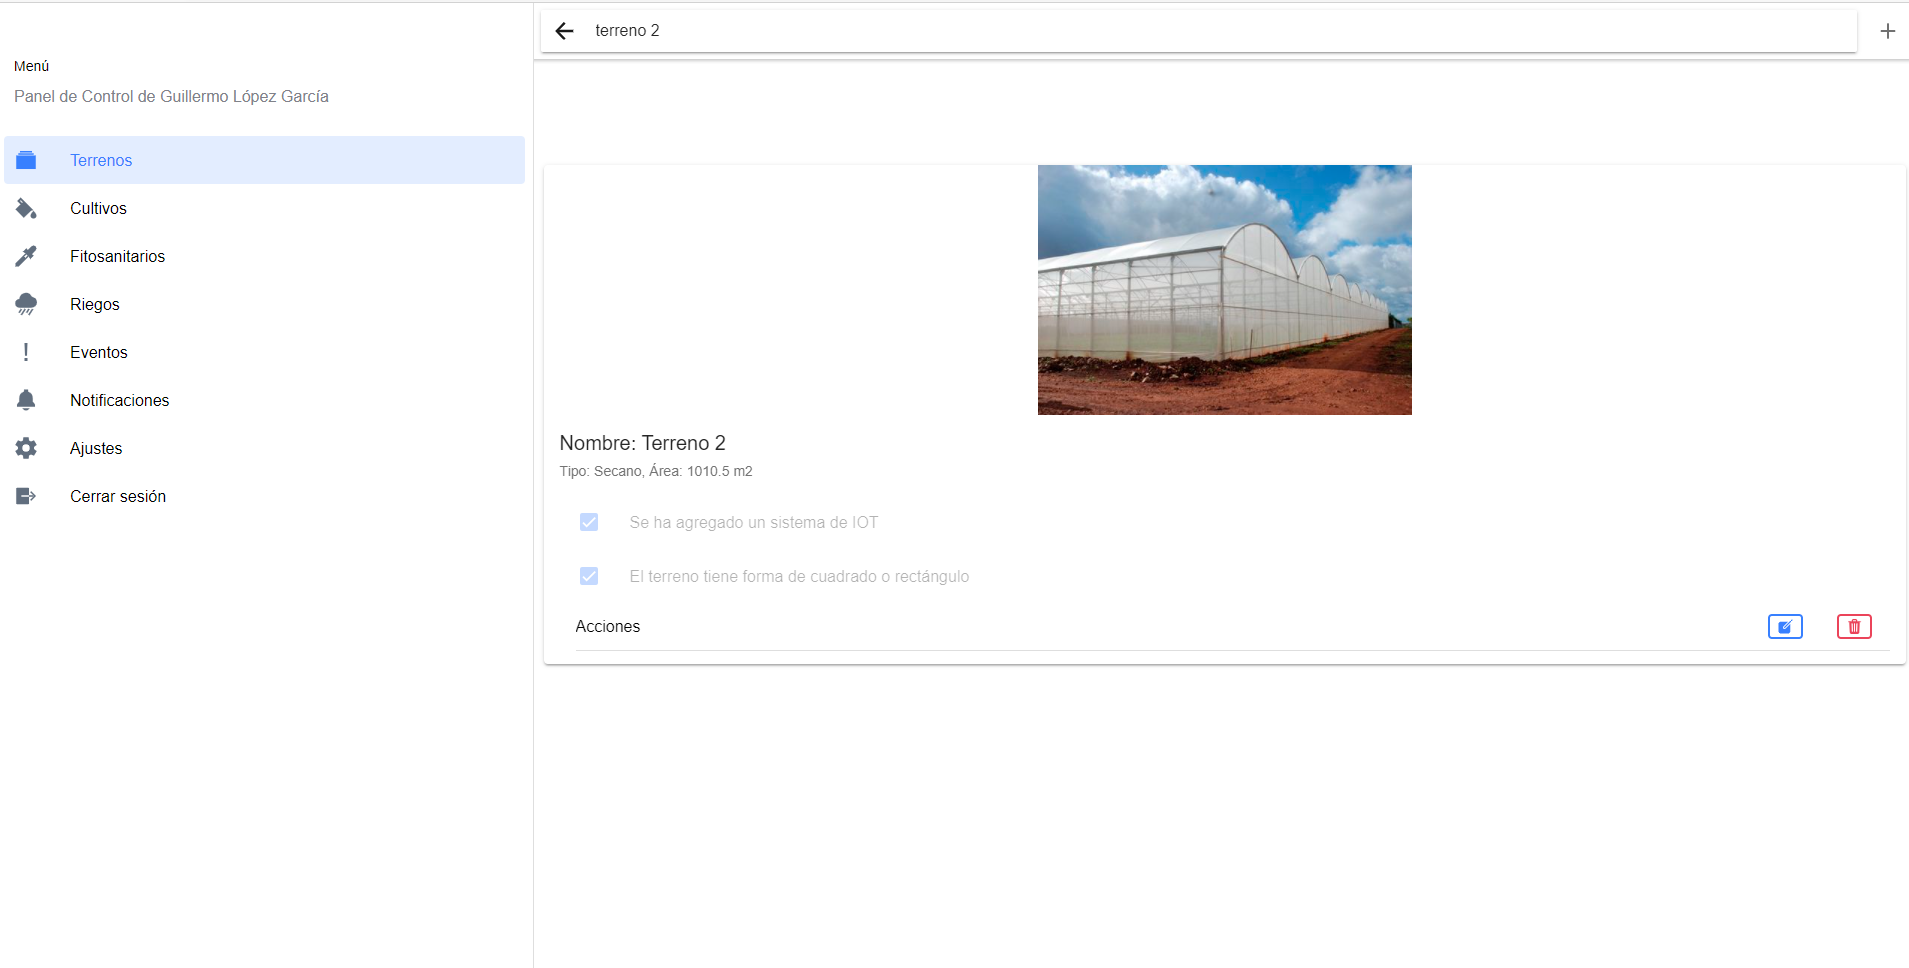
\includegraphics[width=0.7\linewidth]{images/user-manual/farmableland/search.png}
    \caption{Buscar Terrenos}
\end{figure}

\subsubsection{Añadir}
Para añadir un terreno, el usuario debe pulsar en el icono con el símbolo ``+'' y le llevará al formulario, que aparece en la Figura 9.7, para añadir un terreno. Una vez que el usuario lo rellene de forma correcta, se creará el terreno correspondiente.
\begin{figure}[H]
    \centering
    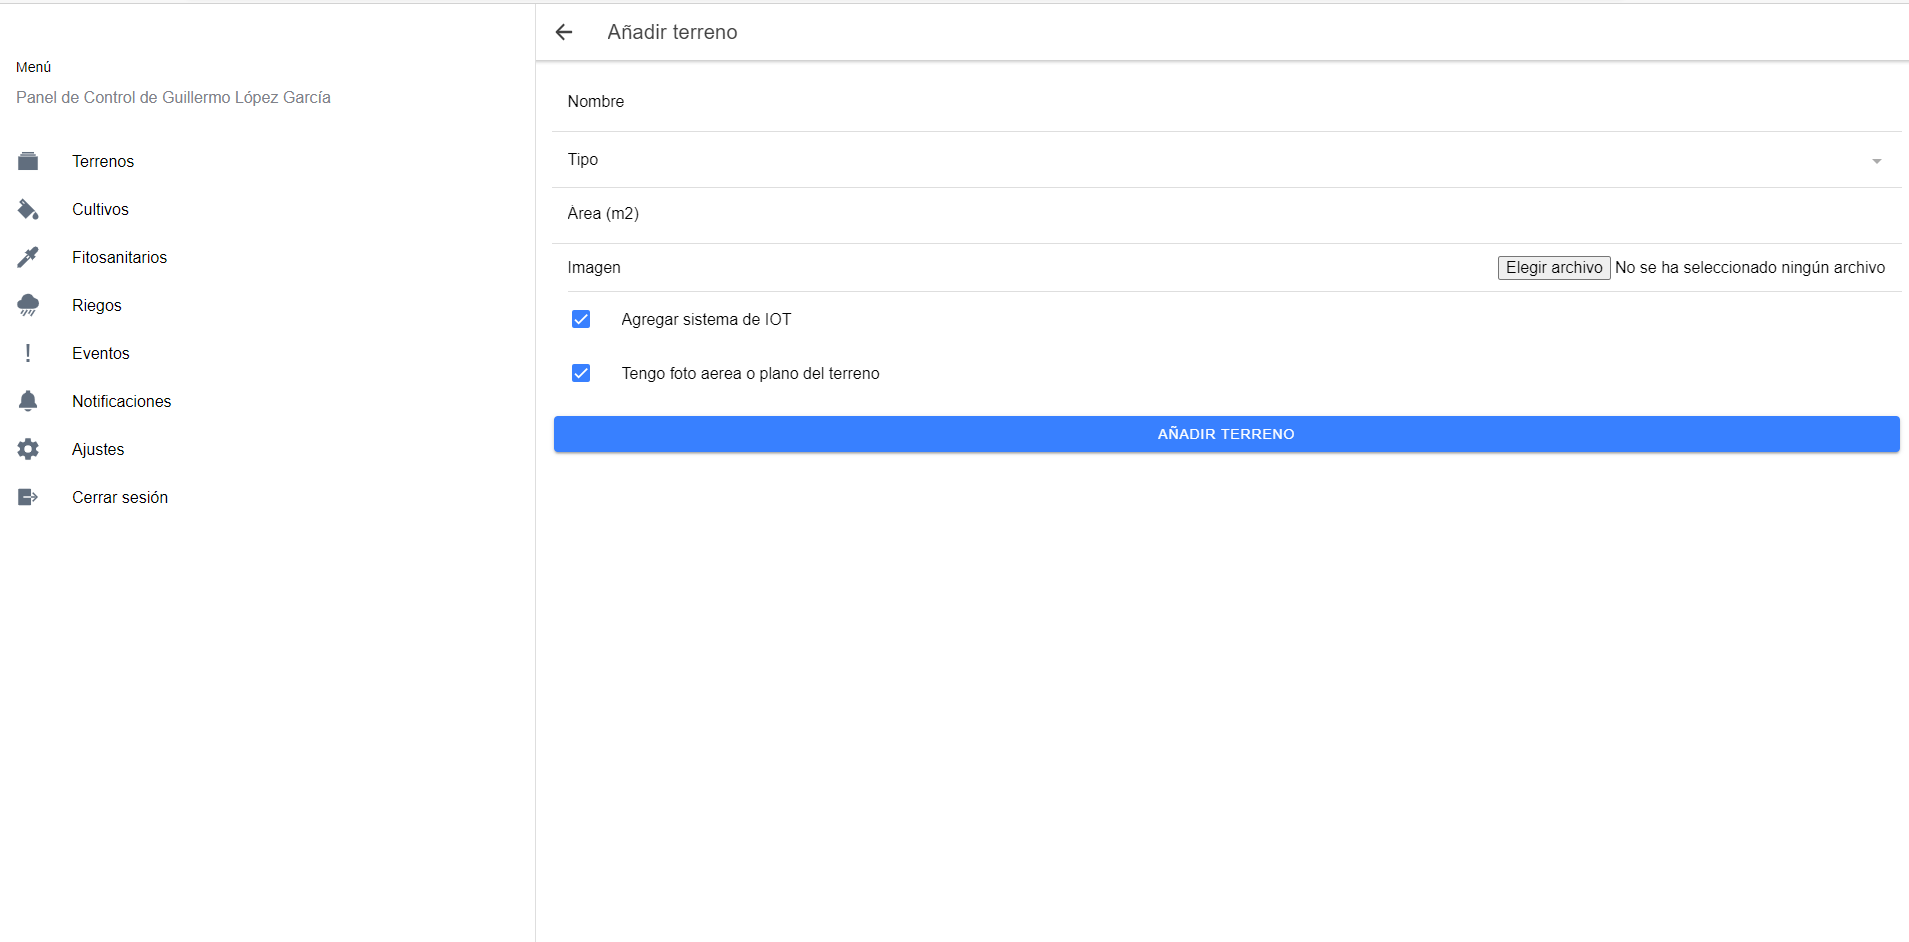
\includegraphics[width=0.7\linewidth]{images/user-manual/farmableland/create.png}
    \caption{Añadir Terreno}
\end{figure}

\subsubsection{Modificar}
Para modificar un terreno, el usuario debe pulsar en icono de editar del terreno y lo llevará al formulario que se puede apreciar en la Figura 9.8. Una vez cambie los valores y además dichos valores sean correctos, el terreno se actualizará.
\begin{figure}[H]
    \centering
    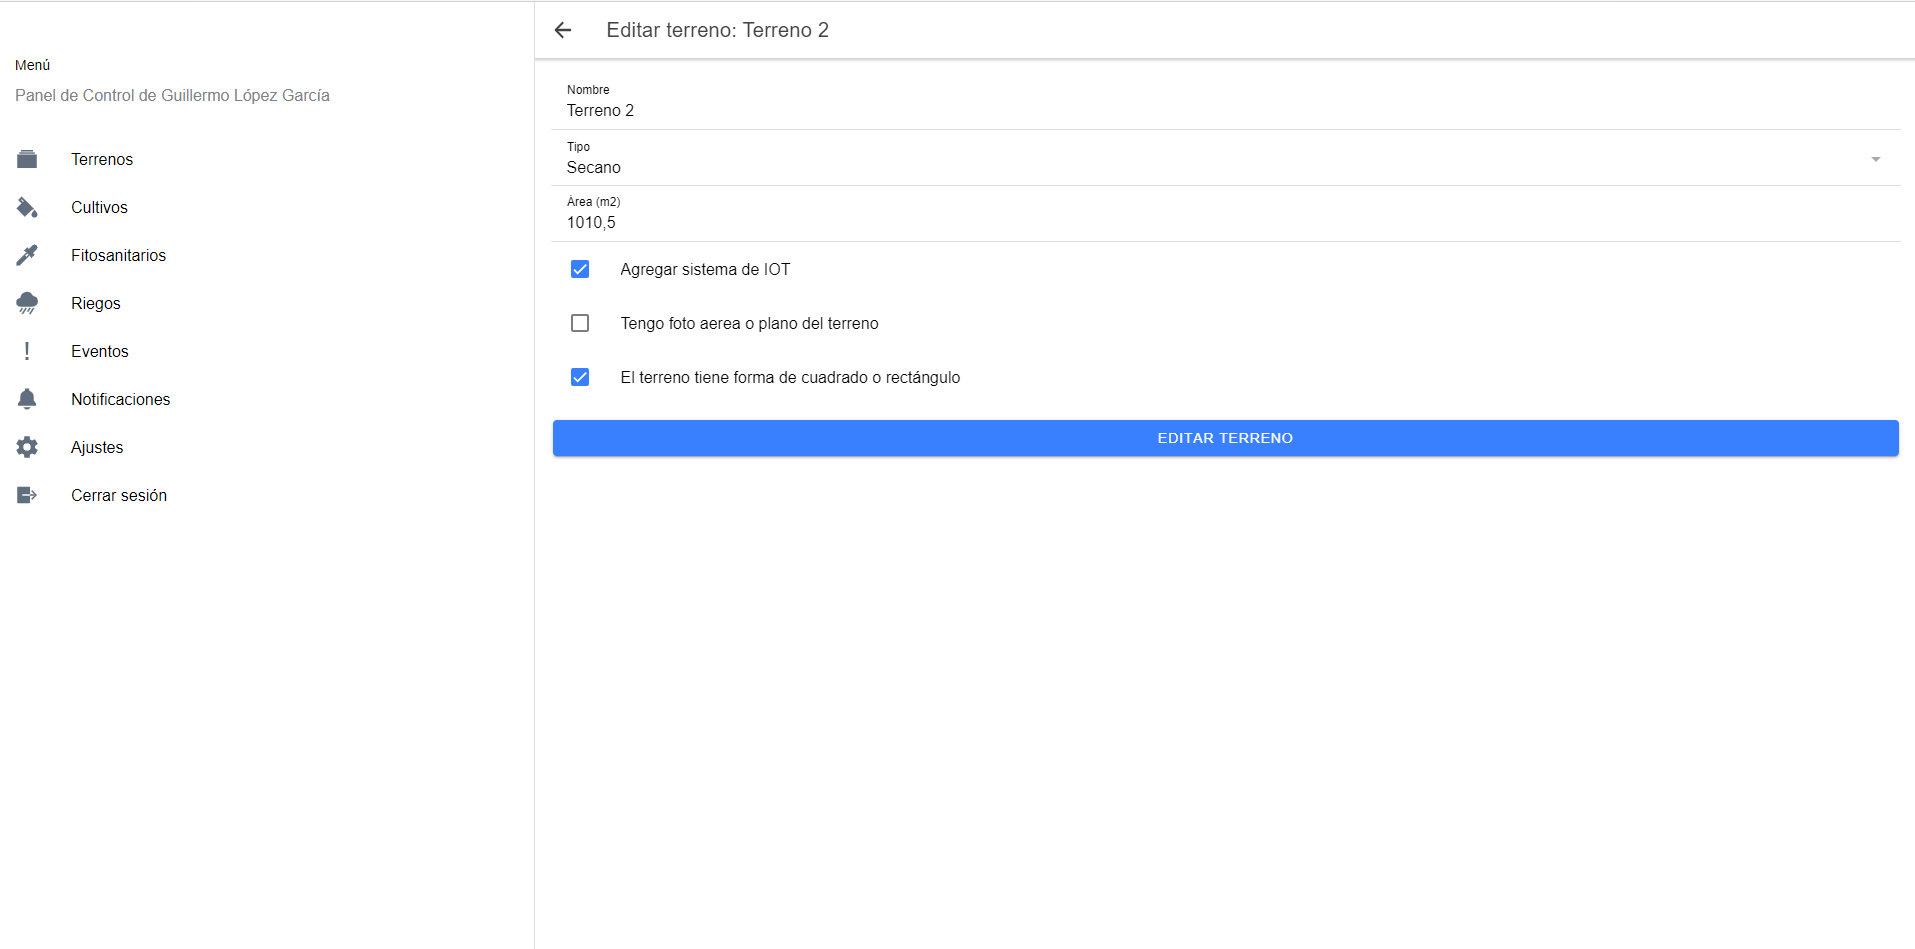
\includegraphics[width=0.7\linewidth]{images/user-manual/farmableland/update.png}
    \caption{Actualizar Terreno}
\end{figure}

\subsubsection{Borrar}
Para borrar un terreno, el usuario debe pulsar en el icono de borrar, el cual aparece resaltado en la Figura 9.9.
Una vez lo pulsé, el terreno se borrará.
\begin{figure}[H]
    \centering
    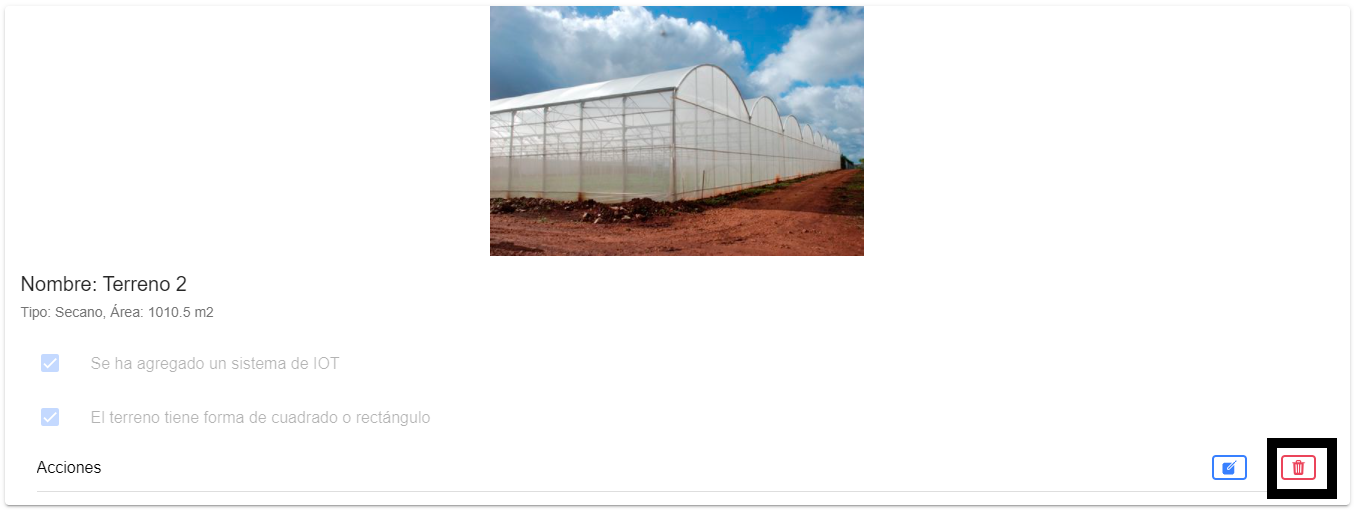
\includegraphics[width=0.7\linewidth]{images/user-manual/farmableland/delete.png}
    \caption{Borrar Terreno}
\end{figure}

\subsection{Cultivos}
En esta sección, se permite todo el CRUD de los cultivos. A continuación, se explica como se hace cada una de las operaciones.

\subsubsection{Listar}
Para listar los cultivos, el usuario debe moverse a la sección de cultivos y directamente se le listará todos los cultivos que posee en sus terrenos, como se puede apreciar en la Figura 9.10.
\begin{figure}[H]
    \centering
    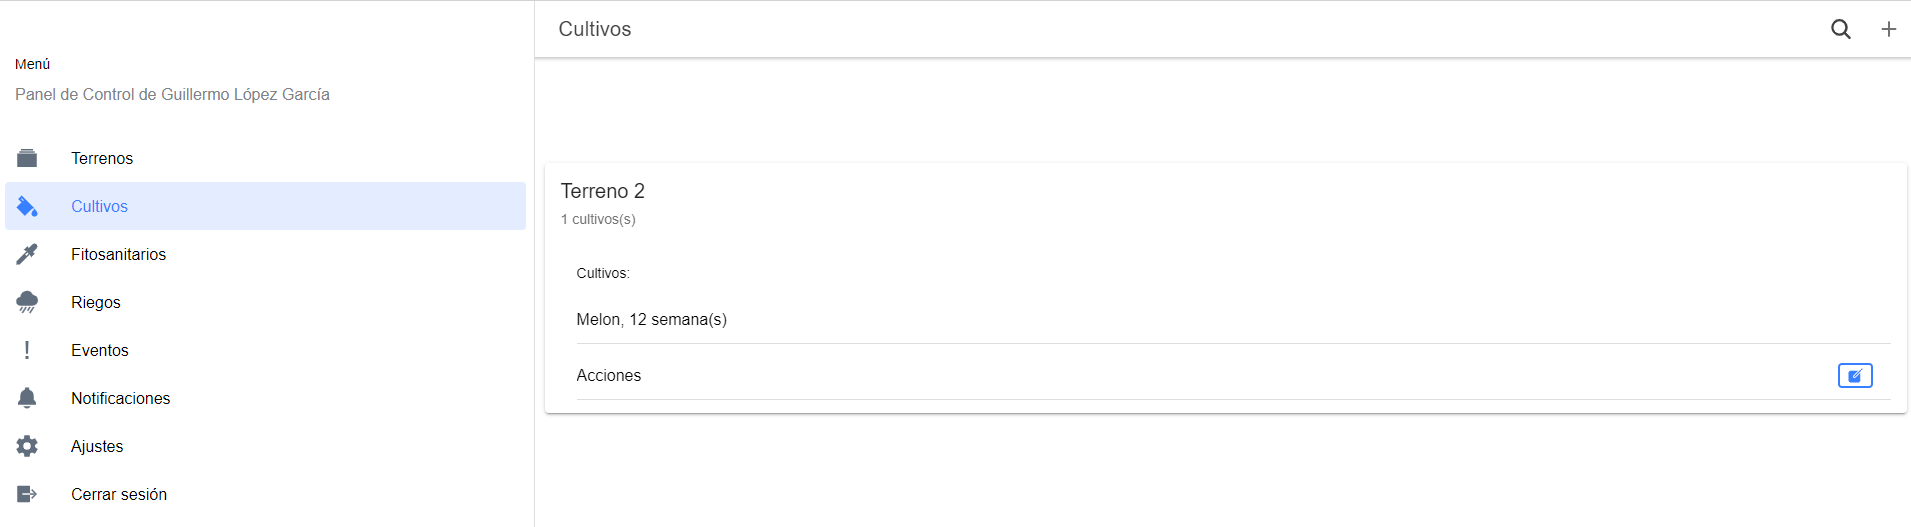
\includegraphics[width=0.7\linewidth]{images/user-manual/crop/list.png}
    \caption{Listar Cultivos}
\end{figure}

\subsubsection{Buscar}
Para buscar un cultivo, el usuario debe pulsar en la barra superior de la sección y escribir la búsqueda deseada. Una vez se escriba la búsqueda, el sistema actualizará el listado de los cultivos automáticamente con el filtro aplicado, como se puede apreciar en la Figura 9.11.
\begin{figure}[H]
    \centering
    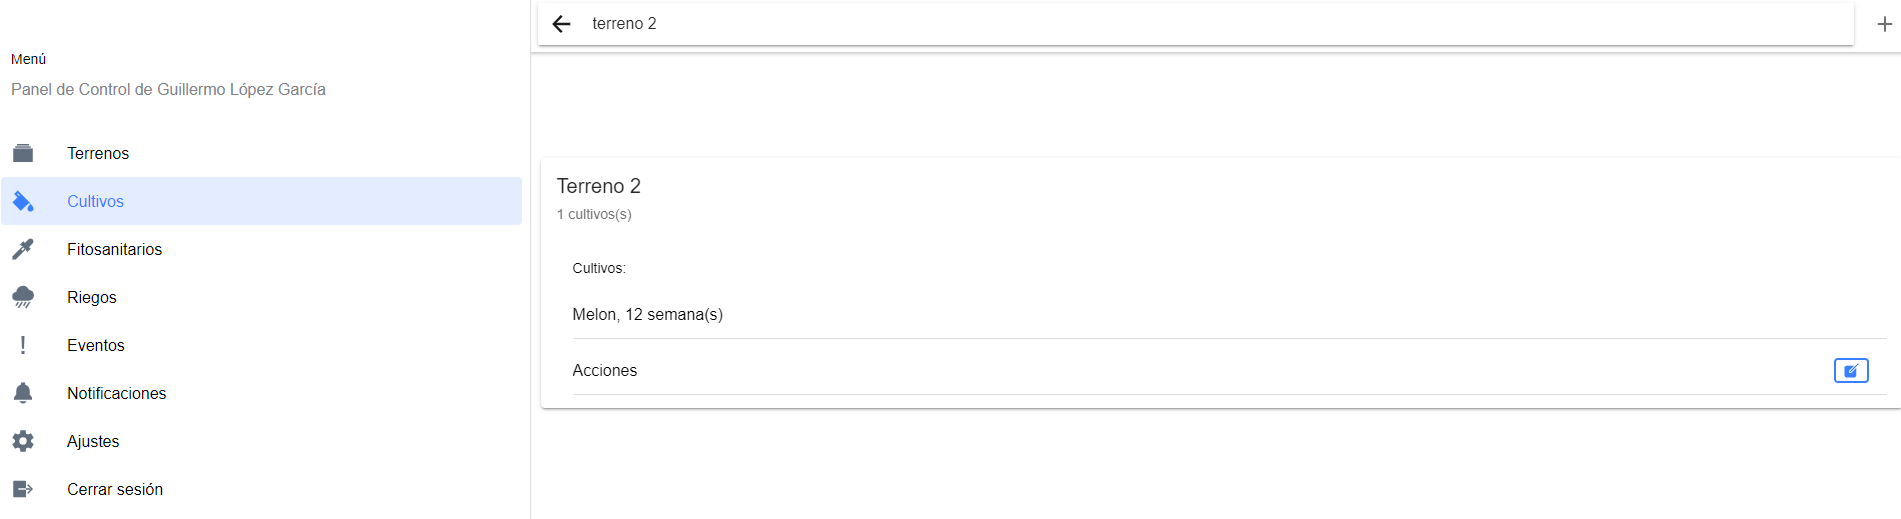
\includegraphics[width=0.7\linewidth]{images/user-manual/crop/search.png}
    \caption{Buscar Cultivos}
\end{figure}

\subsubsection{Añadir}
Para añadir un cultivo, el usuario debe pulsar en el icono con el símbolo ``+'' y el sistema le llevará al formulario correspondiente para crear un cultivo, como se puede apreciar en la Figura 9.12. Una vez complete todos los campos de forma correcta, el sistema guardará el cultivo.
\begin{figure}[H]
    \centering
    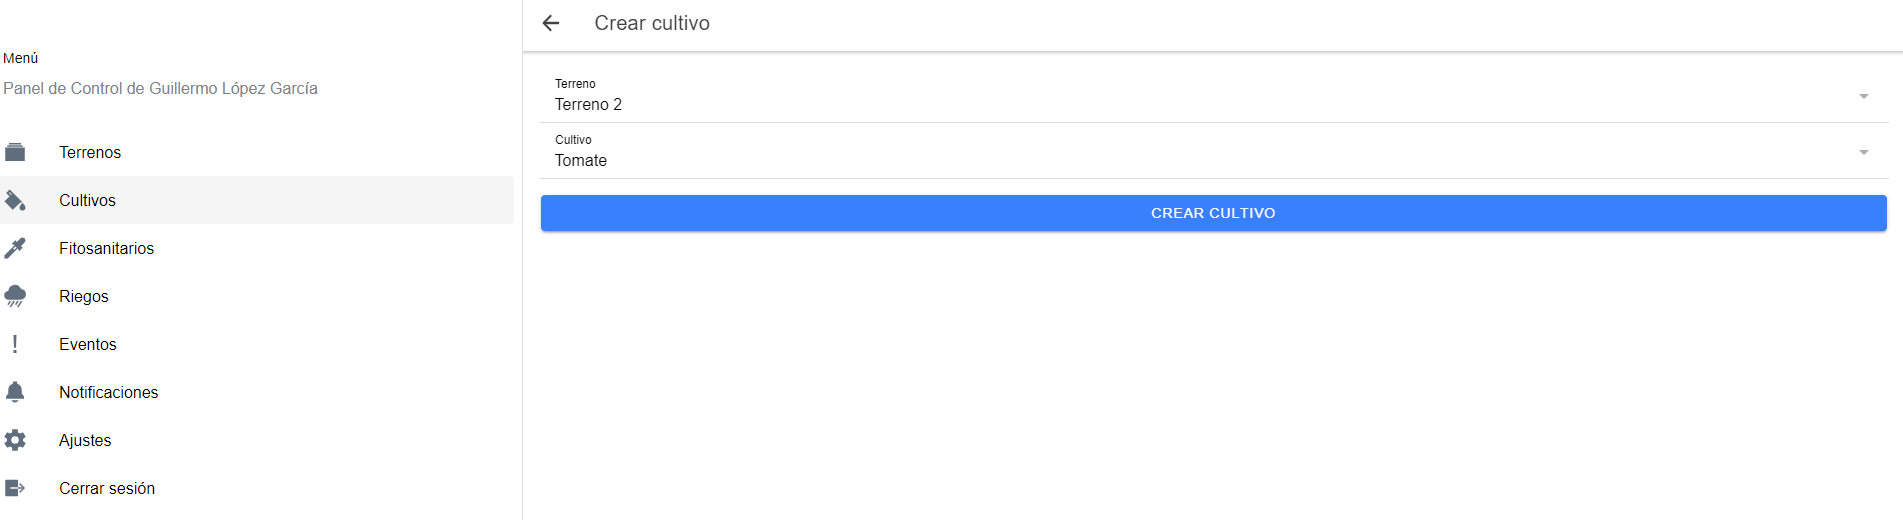
\includegraphics[width=0.7\linewidth]{images/user-manual/crop/create.png}
    \caption{Añadir Cultivo}
\end{figure}

\subsubsection{Modificar}
Para modificar un cultivo, el usuario debe pulsar sobre el icono de editar y el sistema le llevará al formulario correspondiente, que se puede apreciar en la Figura 9.13. Una vez que el usuario edite de forma correcta los campos, el sistema modificará el cultivo.
\begin{figure}[H]
    \centering
    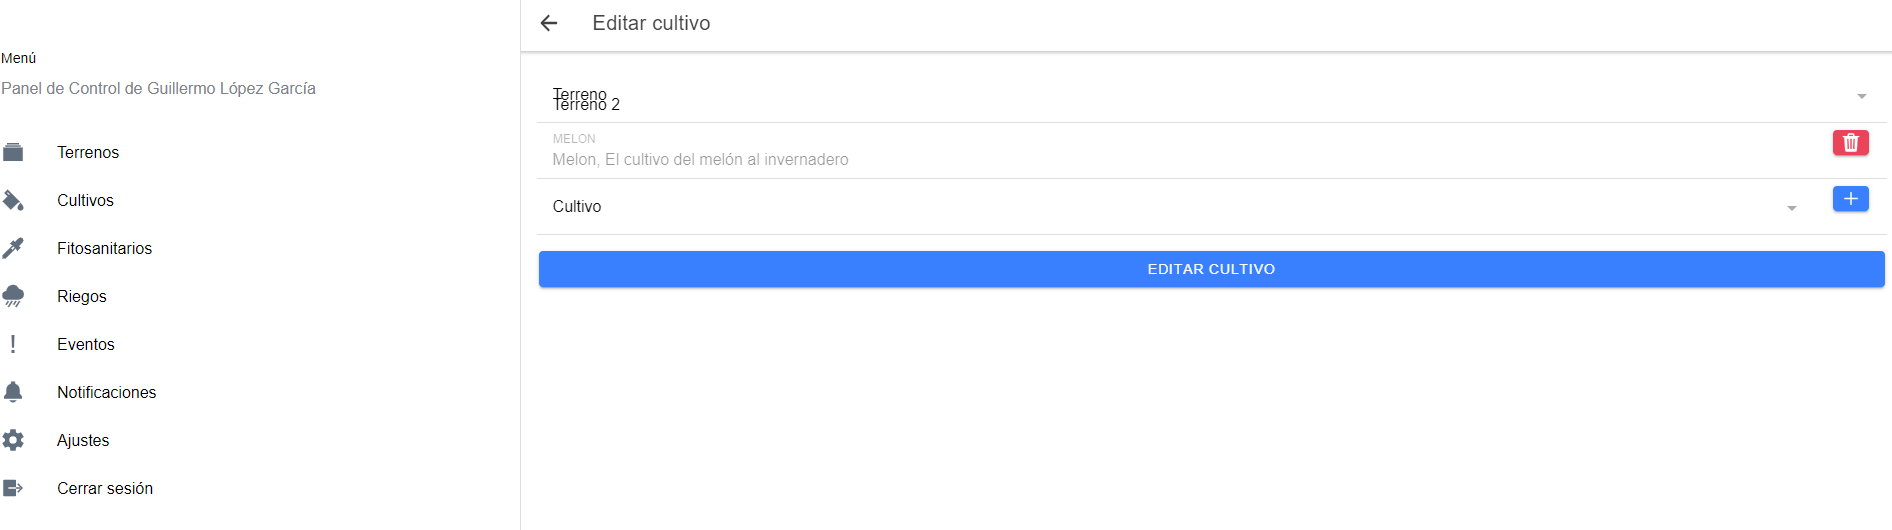
\includegraphics[width=0.7\linewidth]{images/user-manual/crop/update.png}
    \caption{Actualizar Cultivo}
\end{figure}

\subsubsection{Borrar}
Para borrar un cultivo, el usuario debe pulsar sobre el icono de borrar resaltado en la Figura 9.14. Una vez se produzca la acción, el sistema borrará el cultivo del terreno seleccionado.
\begin{figure}[H]
    \centering
    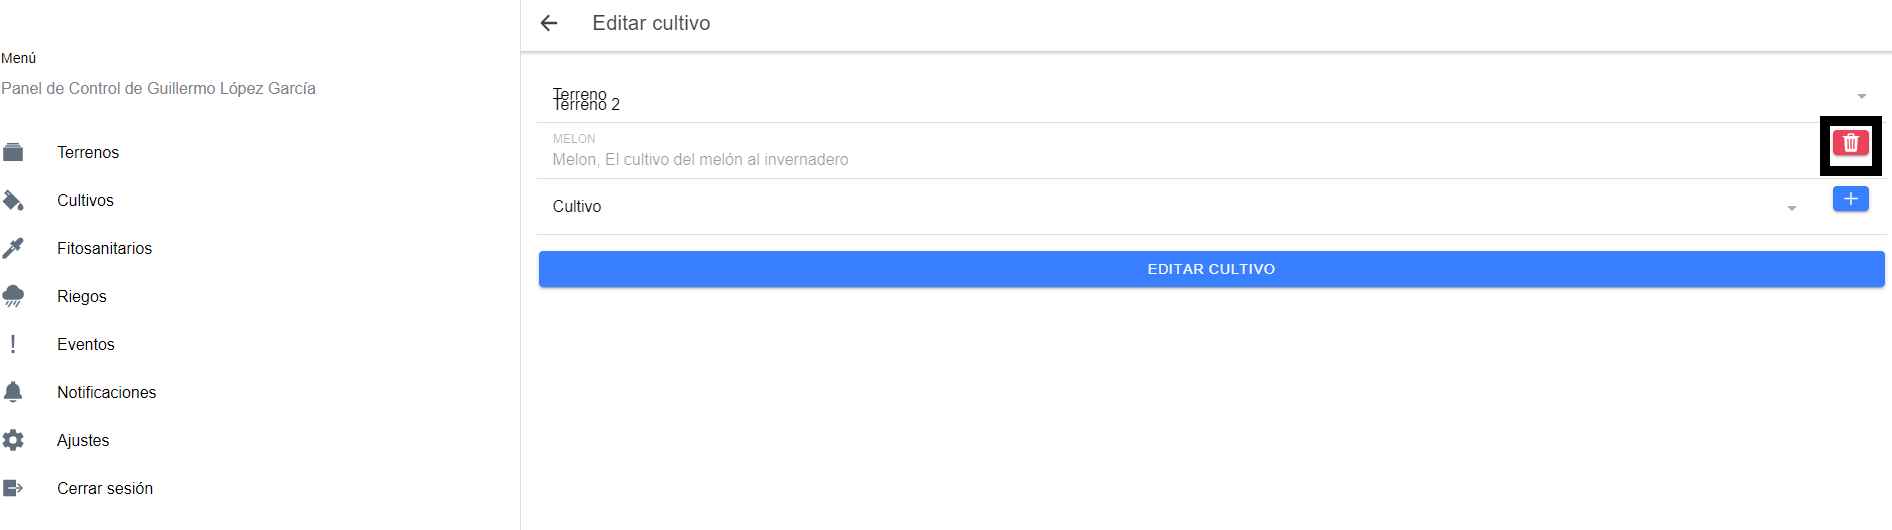
\includegraphics[width=0.7\linewidth]{images/user-manual/crop/delete.png}
    \caption{Borrar Cultivo}
\end{figure}

\subsection{Fitosanitarios}
En esta sección, se permite todo el CRUD de los fitosanitarios. A continuación, se explica como se hace cada una de las operaciones.

\subsubsection{Listar}
Para listar fitosanitarios, el usuario debe moverse a la sección de fitosanitarios pulsando la opción en el menú lateral. Una vez entre, directamente el sistema le listará los fitosanitarios aplicados en cada terreno y en cada cultivo, como se puede apreciar en la Figura 9.15.
\begin{figure}[H]
    \centering
    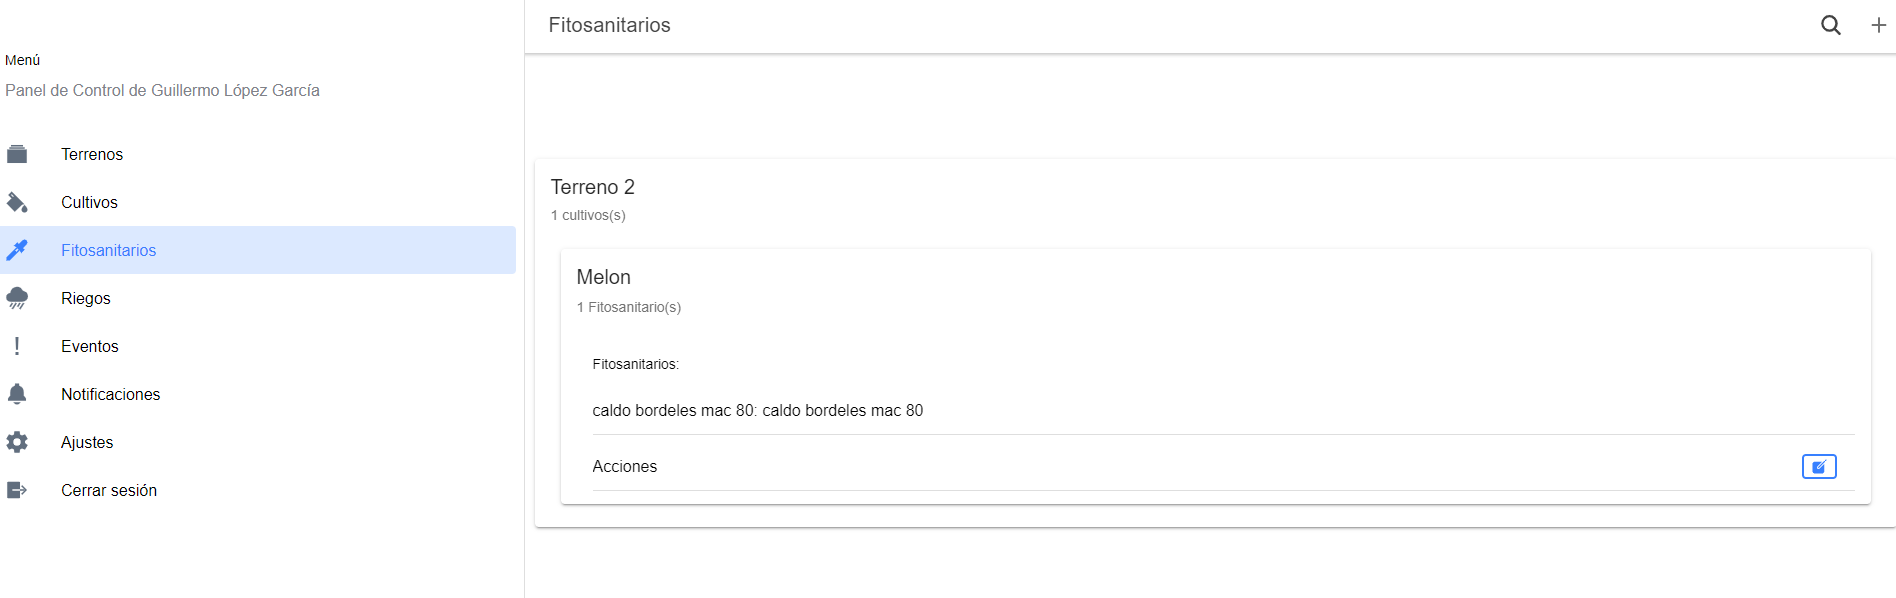
\includegraphics[width=0.7\linewidth]{images/user-manual/phytosanitary/list.png}
    \caption{Listar Fitosanitarios}
\end{figure}

\subsubsection{Buscar}
Para buscar fitosanitarios, el usuario debe pulsar en la barra superior de la sección y escribir el patrón de búsqueda deseado. Una vez lo haga, el sistema automáticamente listará los fitosanitarios con el filtro aplicado, como se puede apreciar en la Figura 9.16.
\begin{figure}[H]
    \centering
    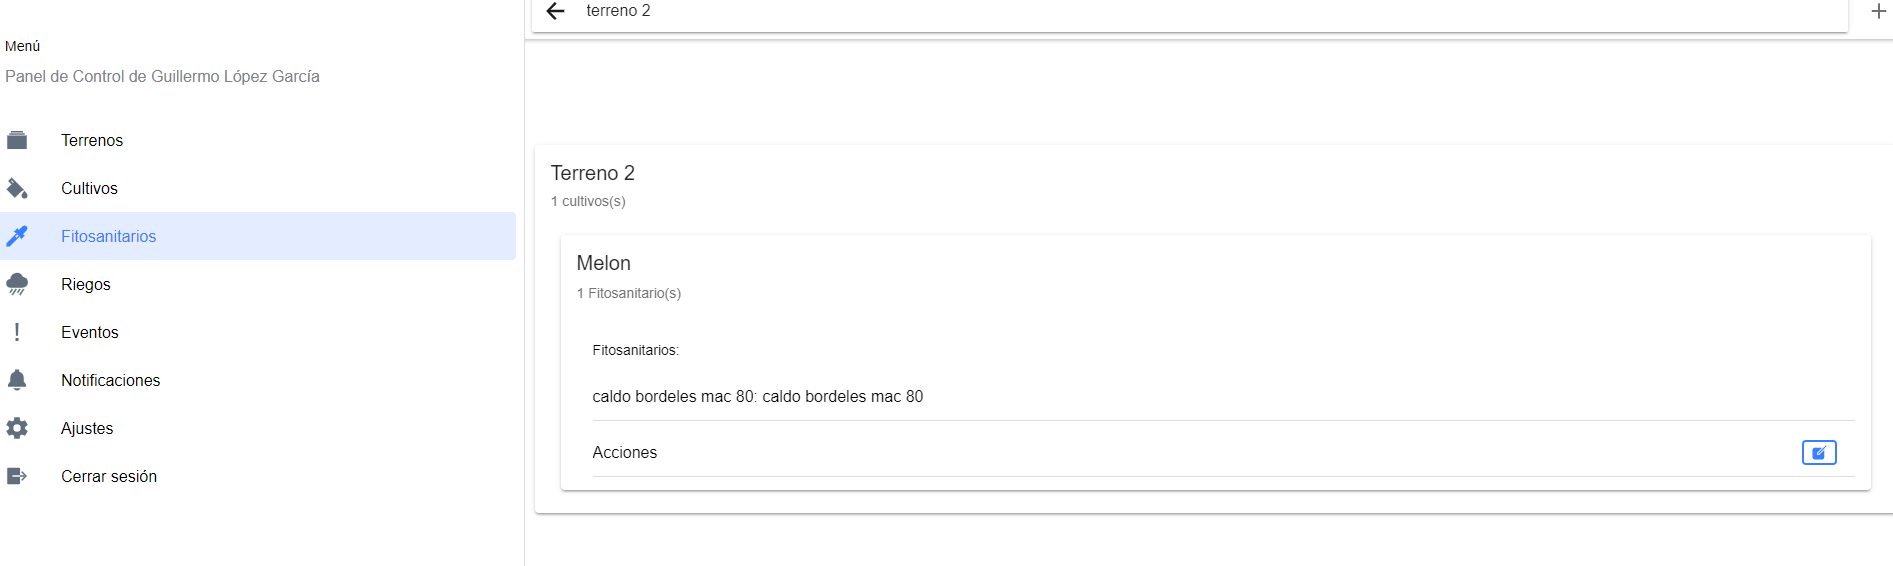
\includegraphics[width=0.7\linewidth]{images/user-manual/phytosanitary/search.png}
    \caption{Buscar Fitosanitarios}
\end{figure}

\subsubsection{Añadir}
Para añadir un fitosanitario, el usuario debe pulsar sobre el icono con el símbolo ``+''. Una vez lo haga, el sistema lo llevará para el formulario correspondiente, que se puede apreciar en la Figura 9.17. Una vez complete todos los campos de forma correcta, se añadirá el fitosanitario.
\begin{figure}[H]
    \centering
    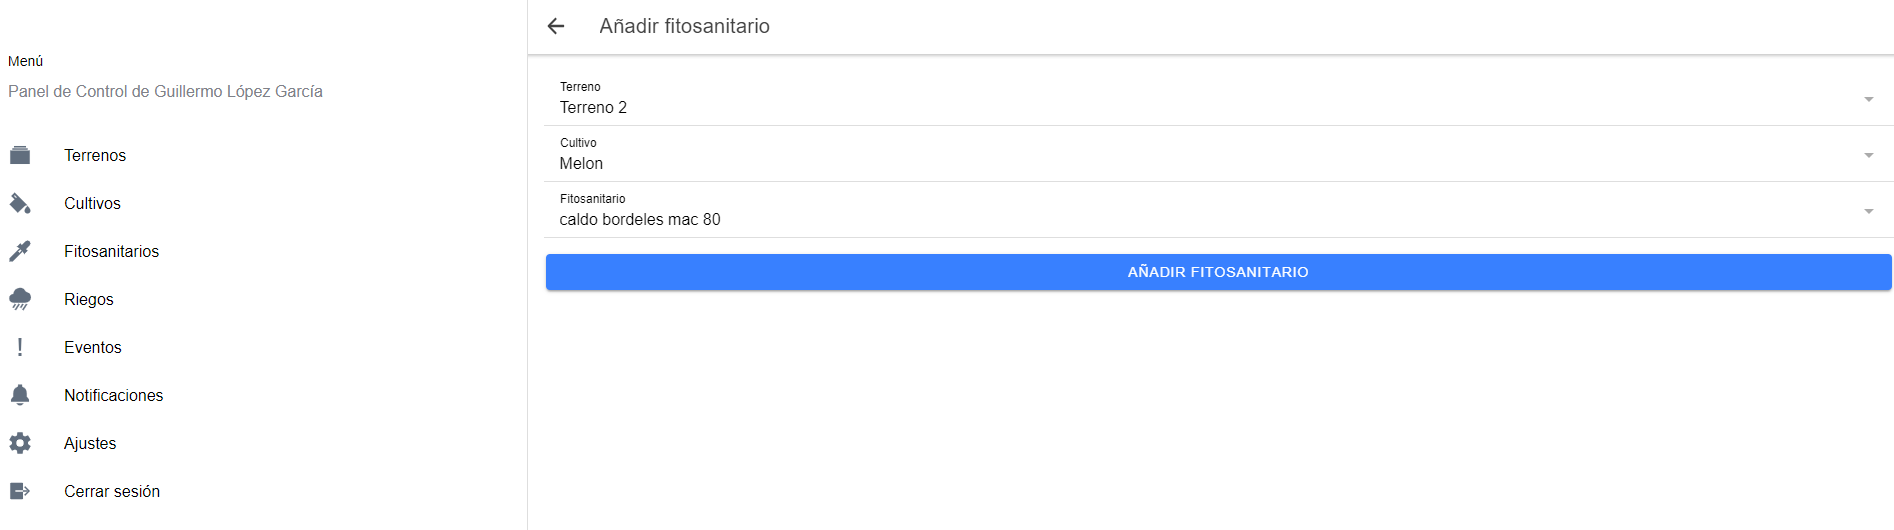
\includegraphics[width=0.7\linewidth]{images/user-manual/phytosanitary/create.png}
    \caption{Añadir Fitosanitario}
\end{figure}

\subsubsection{Modificar}
Para modificar un fitosanitario, el usuario debe pulsar sobre el icono de editar. Una vez lo haga, el sistema lo enviará al formulario correspondiente, que se puede apreciar en la Figura 9.18. Cuando el usuario modifique los campos que desee de forma correcta, el sistema guardará al fitosanitario.
\begin{figure}[H]
    \centering
    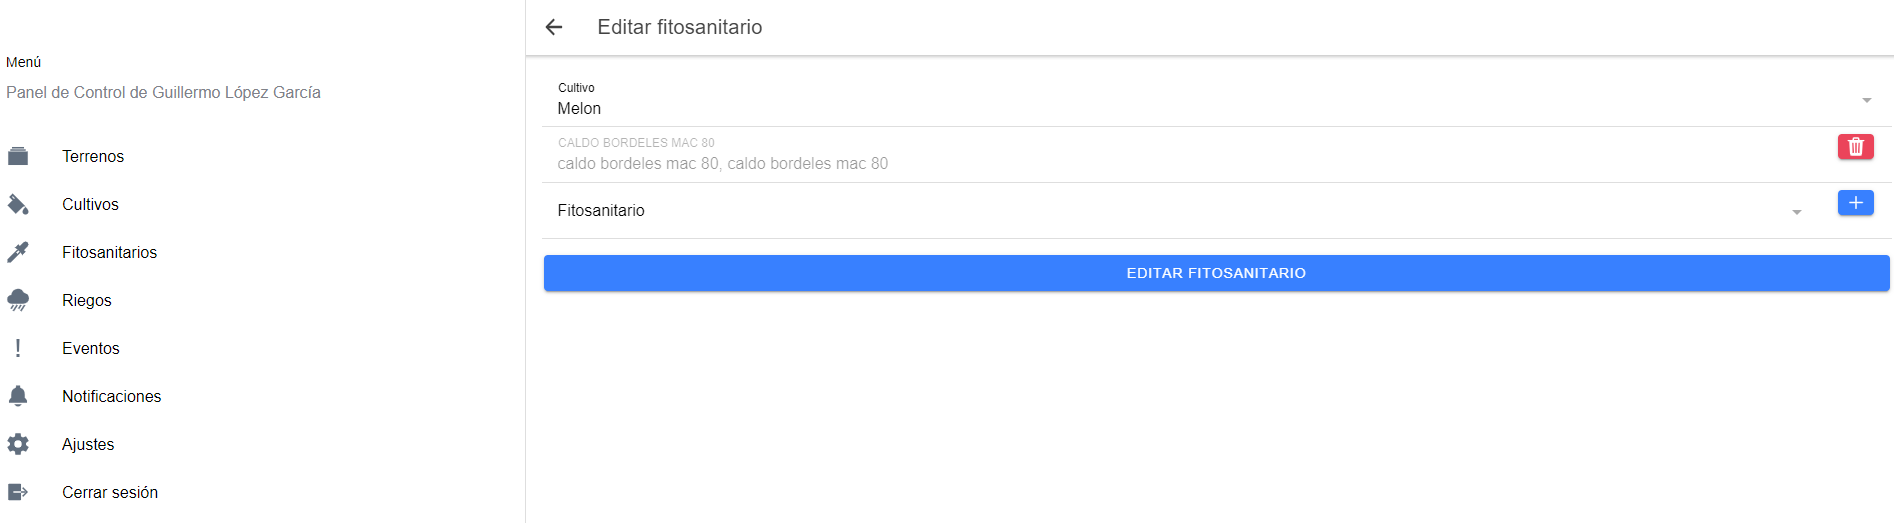
\includegraphics[width=0.7\linewidth]{images/user-manual/phytosanitary/update.png}
    \caption{Actualizar Fitosanitario}
\end{figure}

\subsubsection{Borrar}
Para borrar un fitosanitario, el usuario debe pulsar sobre el icono de borrar, el cual está resaltado en la Figura 9.19. Una vez el usuario pulse sobre el icono, el fitosanitario se borrará.
\begin{figure}[H]
    \centering
    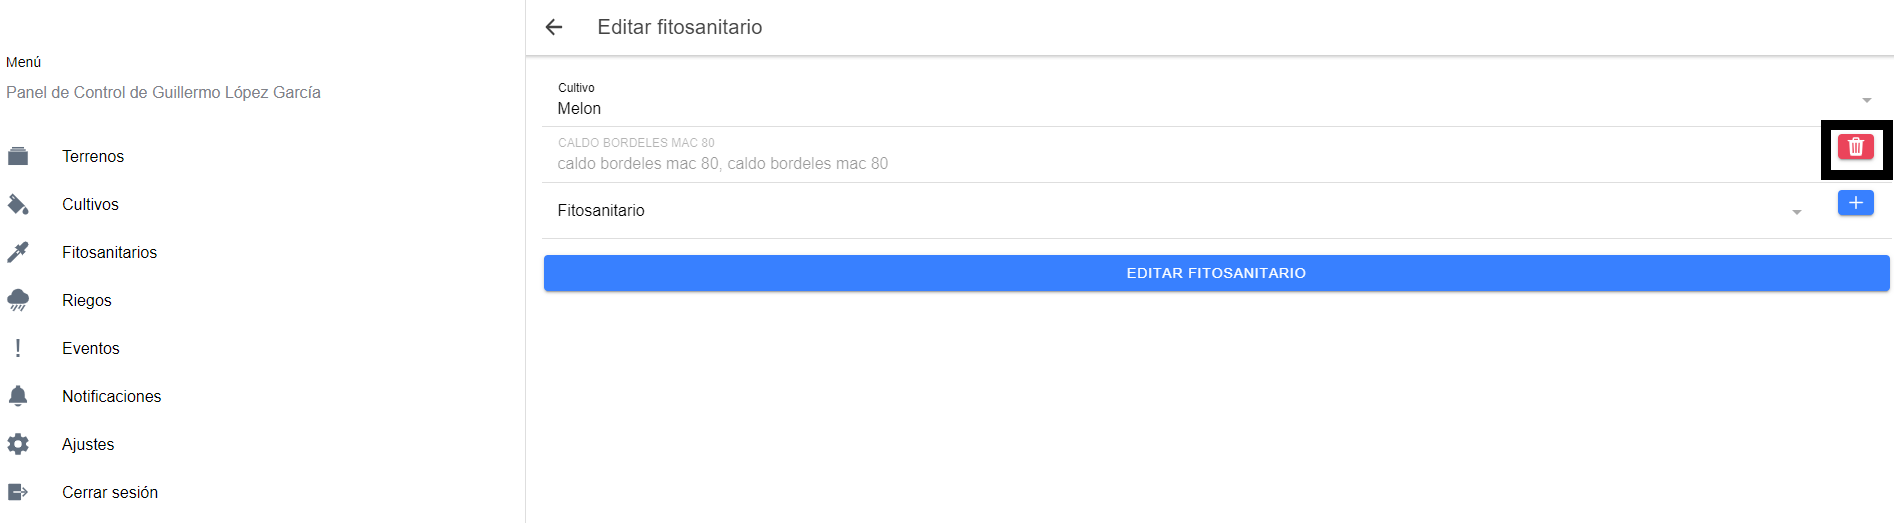
\includegraphics[width=0.7\linewidth]{images/user-manual/phytosanitary/delete.png}
    \caption{Borrar Fitosanitario}
\end{figure}

\subsection{Riegos}
En esta sección, se permite todo el CRUD de los riegos. A continuación, se explica como se hace cada una de las operaciones.

\subsubsection{Listar}
Para listar los riegos, el usuario debe moverse a la sección mediante el menú lateral. Una vez entre en dicha sección, el sistema automáticamente mostrará todos los riegos del usuario, como se puede apreciar en la Figura 9.20.
\begin{figure}[H]
    \centering
    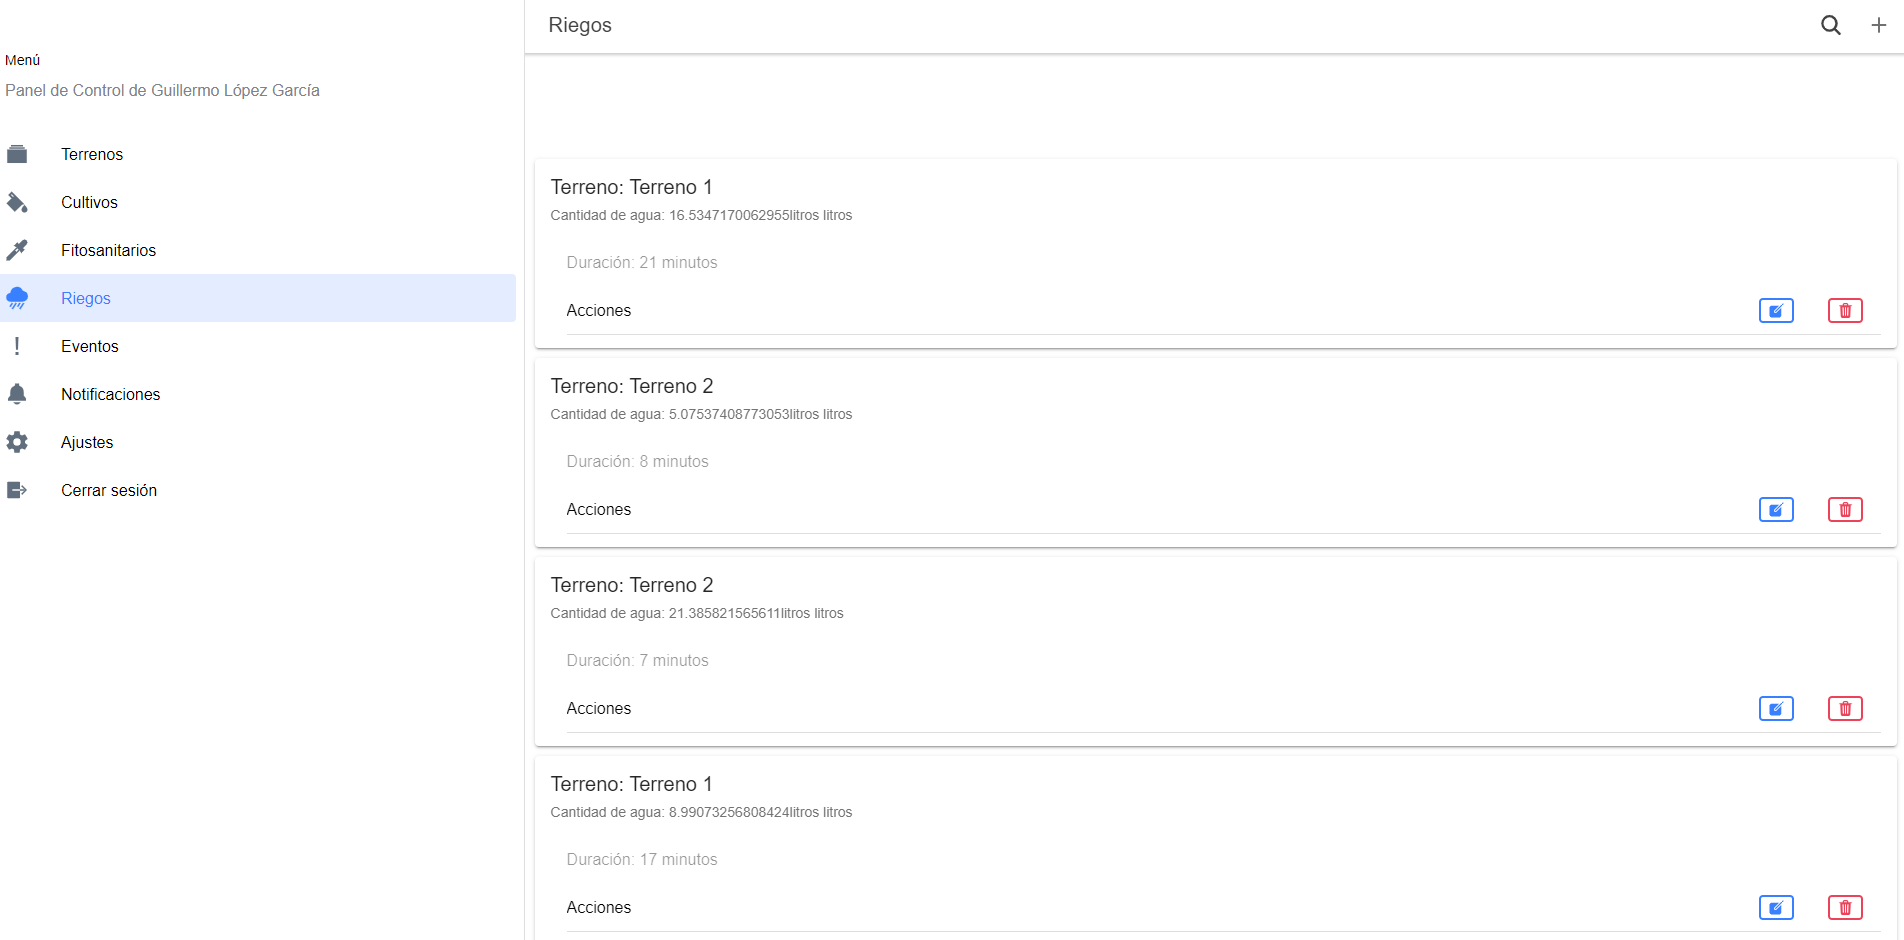
\includegraphics[width=0.7\linewidth]{images/user-manual/irrigate/list.png}
    \caption{Listar Riegos}
\end{figure}

\subsubsection{Buscar}
Para buscar riegos, el usuario debe pulsar sobre la barra superior de la sección y escribir la búsqueda deseada. El sistema, automáticamente, volverá a listar los riegos con el filtro aplicado, como se puede apreciar en la Figura 9.21.
\begin{figure}[H]
    \centering
    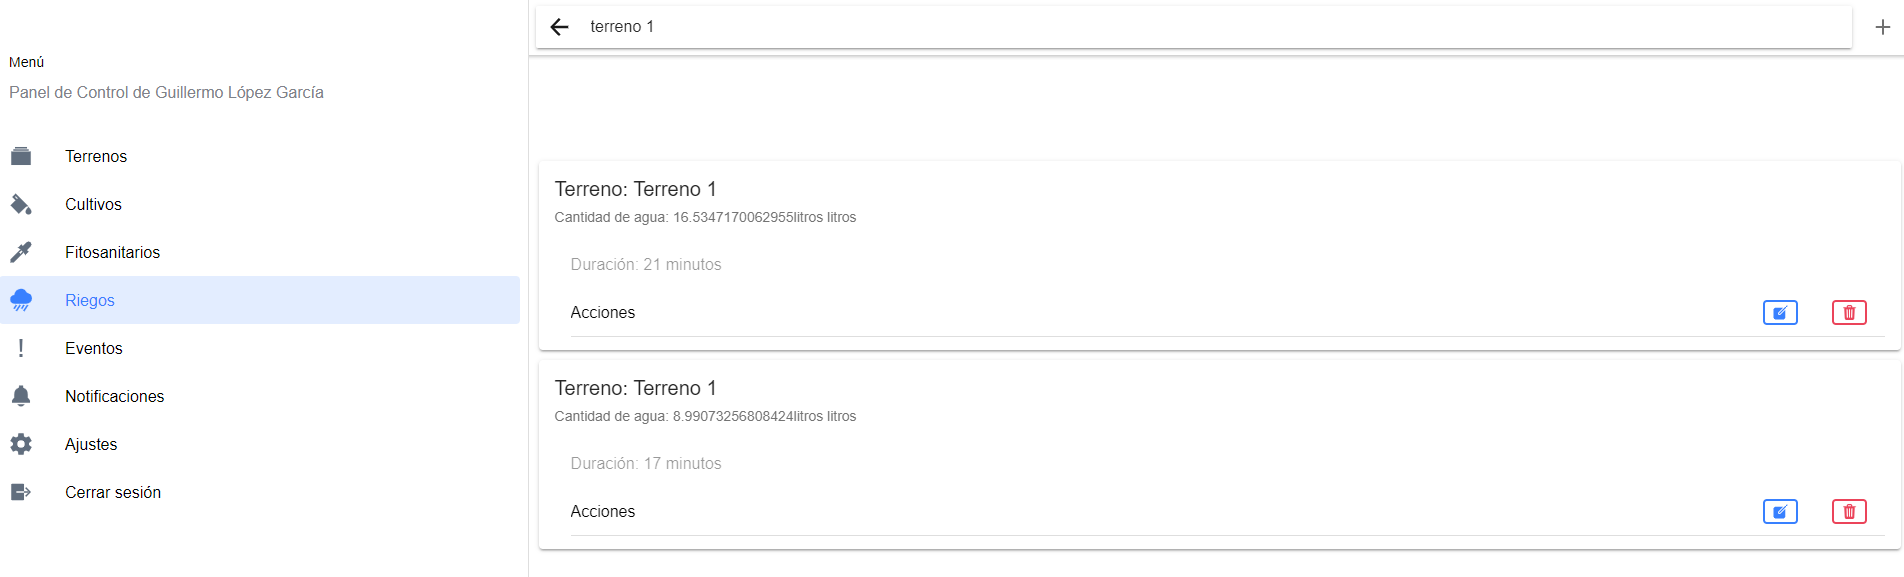
\includegraphics[width=0.7\linewidth]{images/user-manual/irrigate/search.png}
    \caption{Buscar Riegos}
\end{figure}

\subsubsection{Añadir}
Para añadir un riego, el usuario debe pulsar sobre el icono con el símbolo ``+'' y el sistema lo llevará al formulario correspondiente, que se puede apreciar en la Figura 9.22. Una vez el usuario rellene los campos de forma correcta, el sistema guardará el riego.
\begin{figure}[H]
    \centering
    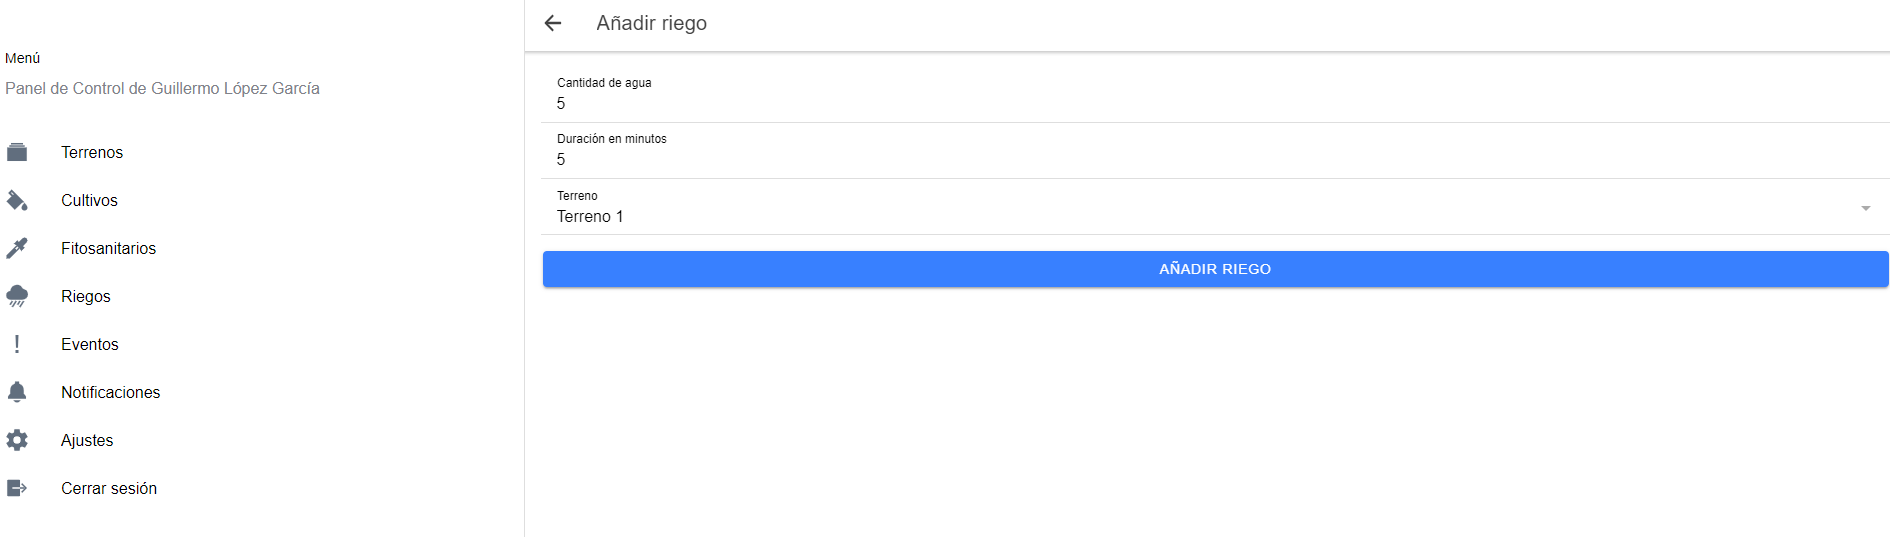
\includegraphics[width=0.7\linewidth]{images/user-manual/irrigate/create.png}
    \caption{Añadir Riego}
\end{figure}

\subsubsection{Modificar}
Para modificar un riego, el usuario debe pulsar sobre el icono de editar, y el sistema llevará al usuario al formulario correspondiente, que se puede apreciar en la Figura 9.23. Una vez el usuario modifique los campos, el sistema guadará el riego modificado.
\begin{figure}[H]
    \centering
    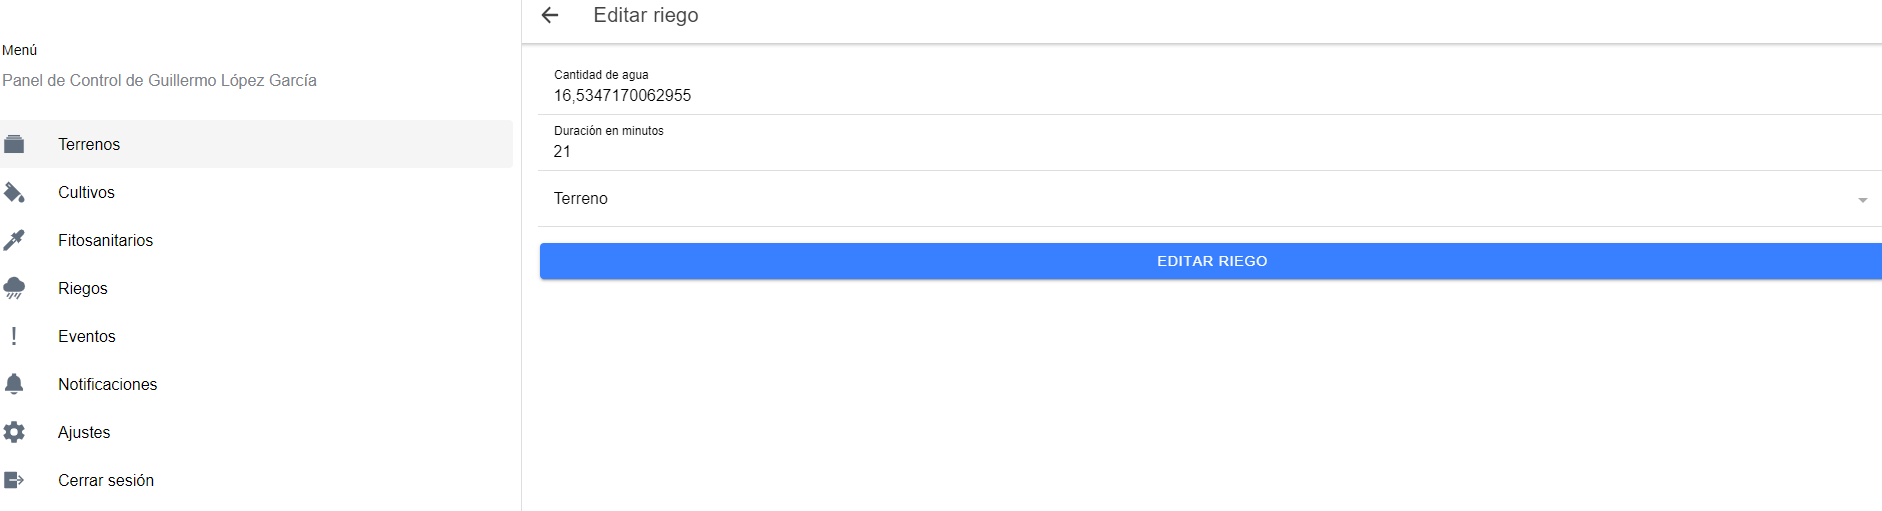
\includegraphics[width=0.7\linewidth]{images/user-manual/irrigate/update.png}
    \caption{Actualizar Riego}
\end{figure}

\subsubsection{Borrar}
Para borrar un riego, el usuario debe pulsar sobre el icono de borrar, resaltado en la Figura 9.24. Una vez pulse en el, el sistema borrará el riego.
\begin{figure}[H]
    \centering
    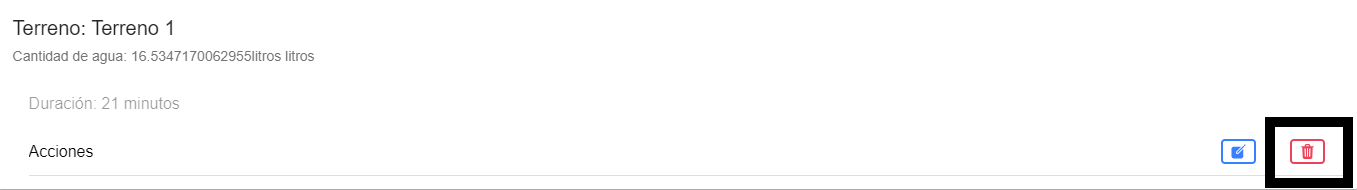
\includegraphics[width=0.7\linewidth]{images/user-manual/irrigate/delete.png}
    \caption{Borrar Riego}
\end{figure}

\subsection{Eventos}
En esta sección, se permite todo el CRUD de los eventos. A continuación, se explica como se hace cada una de las operaciones.

\subsubsection{Listar}
Para listar los eventos a los que está suscrito, el usuario deberá moverse a la sección de eventos. Una vez entre en la sección, el sistema automáticamente listará todos los eventos complejos a los que está suscrito el usuario. Esto se puede apreciar en la Figura 9.25.
\begin{figure}[H]
    \centering
    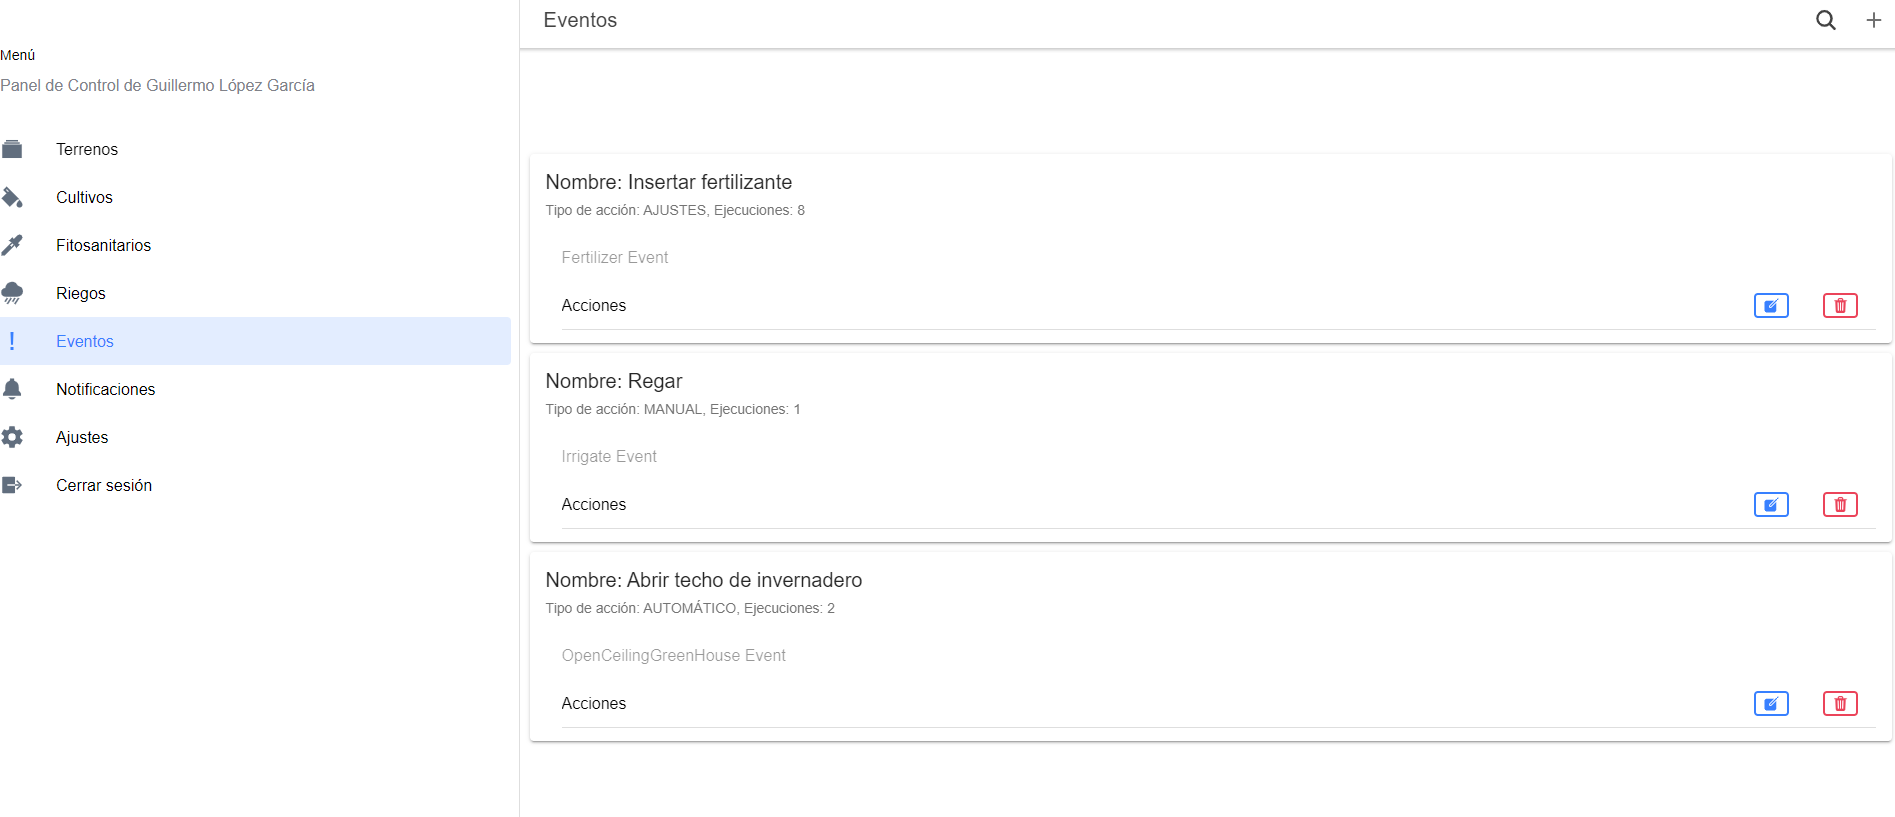
\includegraphics[width=0.7\linewidth]{images/user-manual/events/list.png}
    \caption{Listar Eventos}
\end{figure}

\subsubsection{Buscar}
Para buscar entre los eventos complejos, el usuario debe pulsar sobre la barra superior de la sección. una vez lo haga, deberá escribir la búsqueda que desea. El sistema automáticamente, listará los eventos con el filtro aplicado, como se puede apreciar en la Figura 9.26.
\begin{figure}[H]
    \centering
    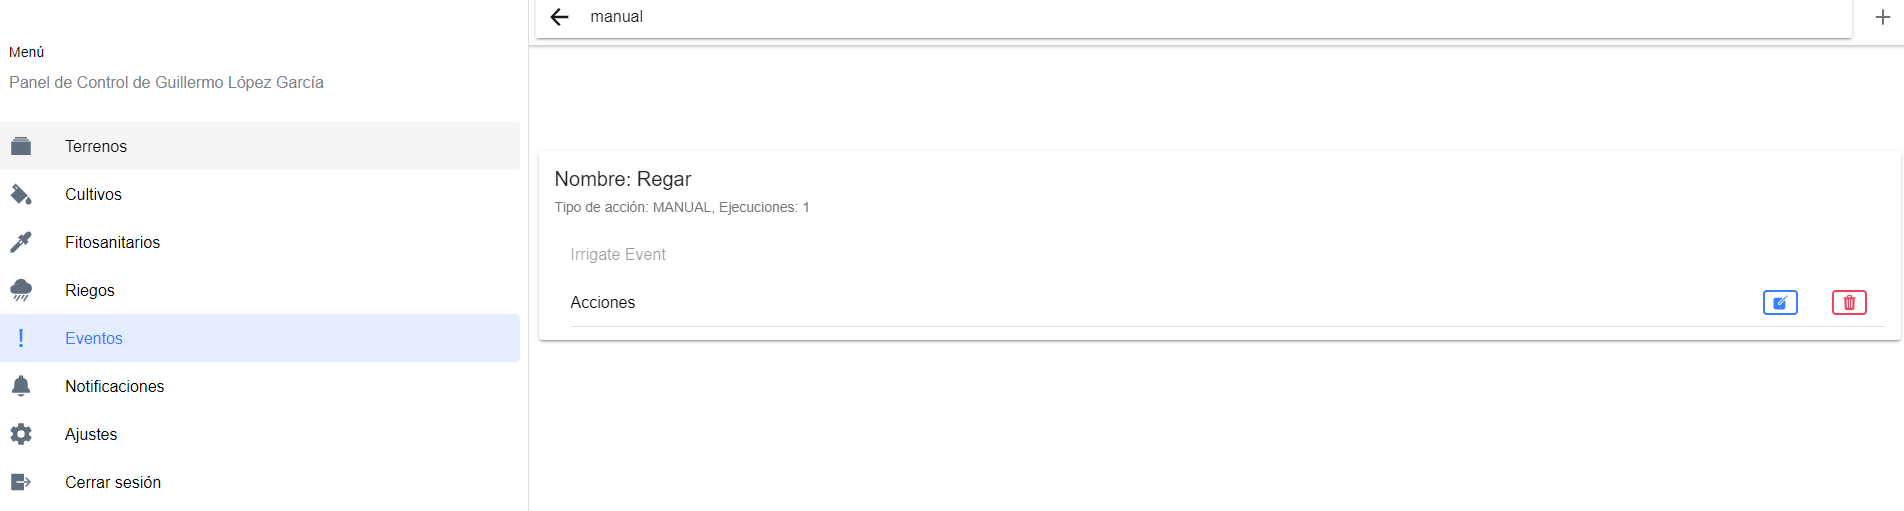
\includegraphics[width=0.7\linewidth]{images/user-manual/events/search.png}
    \caption{Buscar Eventos}
\end{figure}

\subsubsection{Añadir}
Para suscribirse a un evento complejo, el usuario deberá pulsar sobre el icono con el símbolo ``+'' y el sistema le llevará al formulario correspondiente como se puede apreciar en la Figura 9.27. Una vez el usuario rellene el formulario correctamente, el sistema guardará la suscripción al evento.
\begin{figure}[H]
    \centering
    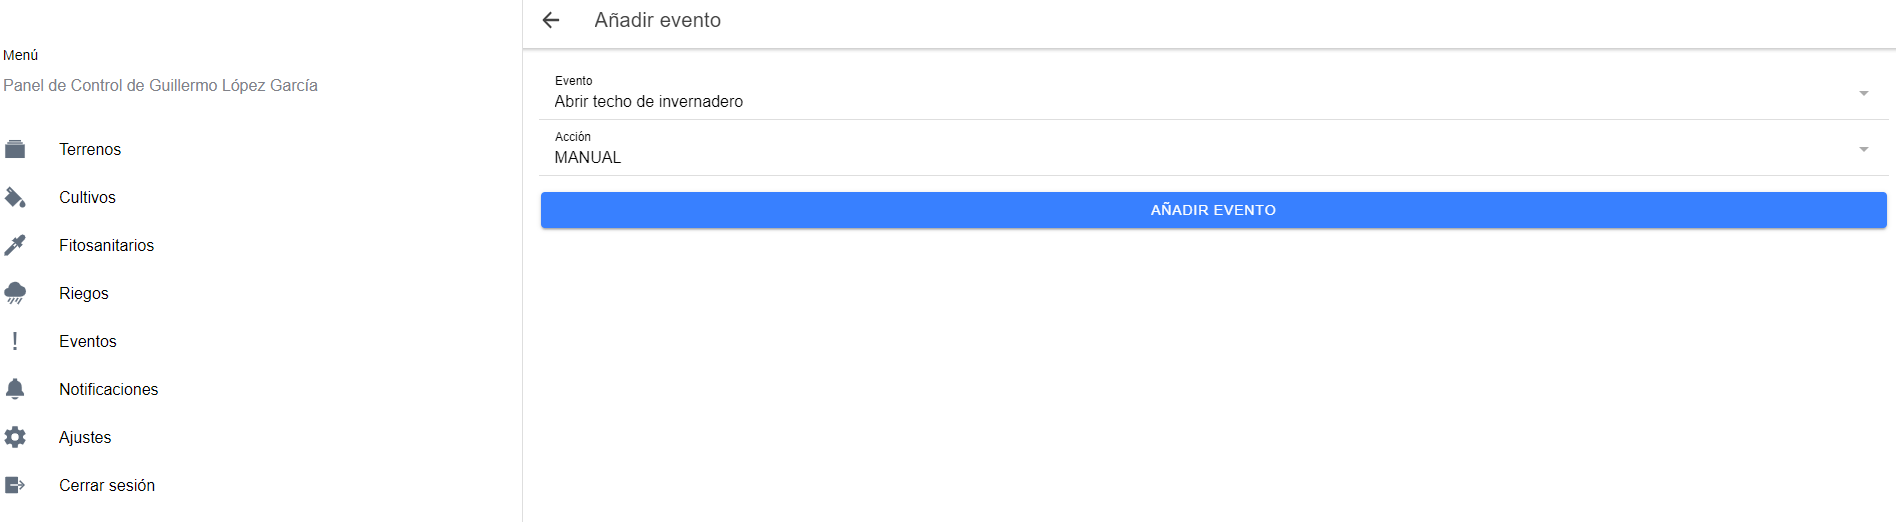
\includegraphics[width=0.7\linewidth]{images/user-manual/events/create.png}
    \caption{Añadir Evento}
\end{figure}

\subsubsection{Modificar}
Para modificar la suscripción a un evento, el usuario deberá pulsar sobre el icono de editar. Una vez pulse, el sistema llevará al usuario al formulario correspondiente que se puede apreciar en la Figura 9.28. Cuando el usuario modifique los campos, el sistema guardará la suscripción modificada.
\begin{figure}[H]
    \centering
    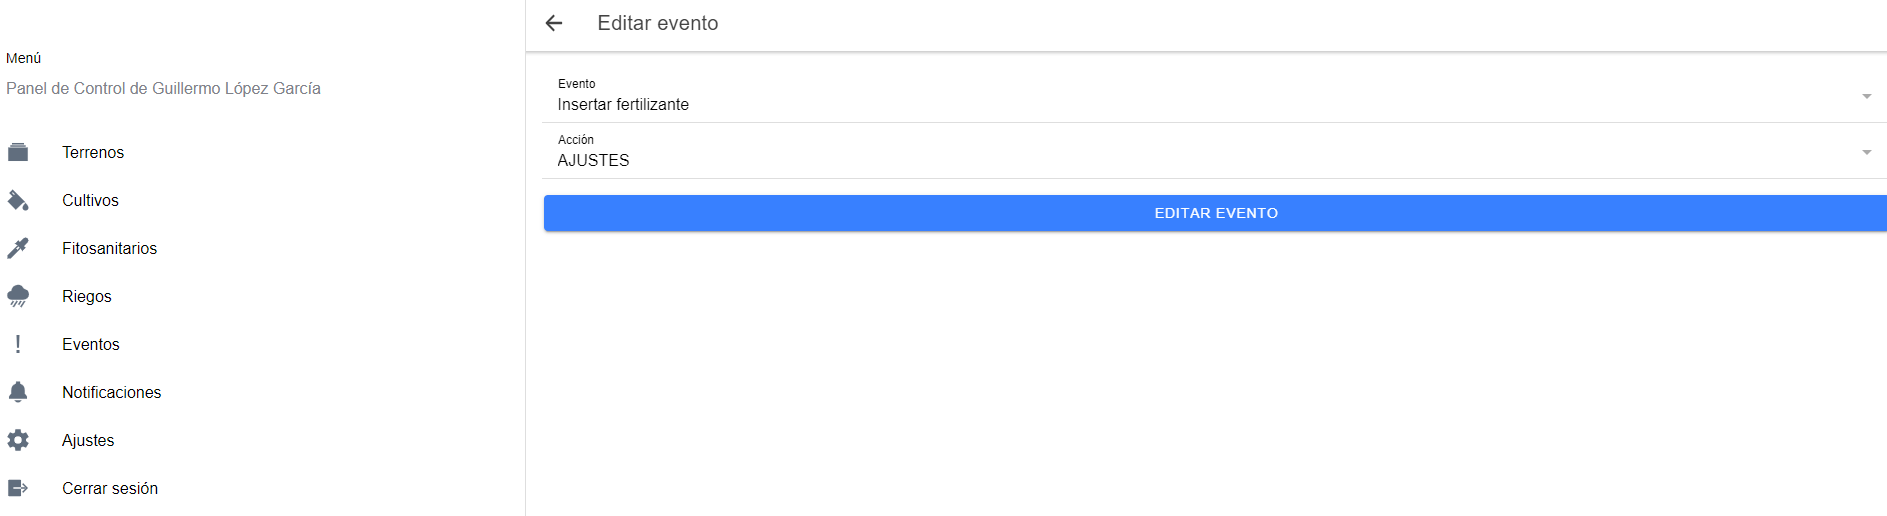
\includegraphics[width=0.7\linewidth]{images/user-manual/events/update.png}
    \caption{Actualizar Evento}
\end{figure}

\subsubsection{Borrar}
Para desuscribirse de un evento complejo, el usuario deberá pulsar sobre el icono de borrar que está resaltado en la Figura 9.29. Una vez el usuario pulse, se borrará la suscripción del usuario a dicho evento complejo.
\begin{figure}[H]
    \centering
    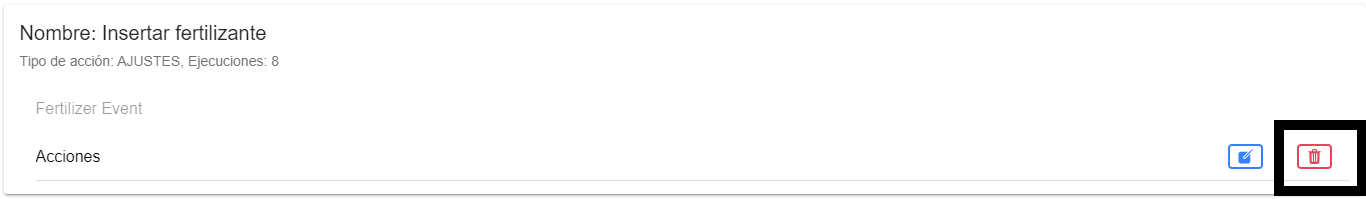
\includegraphics[width=0.7\linewidth]{images/user-manual/events/delete.png}
    \caption{Borrar Evento}
\end{figure}

\subsection{Notificaciones}
En esta sección, se permite listar todo el histórico de notificaciones del usuario.

\subsubsection{Listar}
Para listar las notificaciones, el usuario deberá moverse a la sección. Una vez se encuentre en ella, el sistema automáticamente mostrará todas las notificaciones del usuario ordenadas de más cercana a más lejana en el tiempo, como se puede apreciar en la Figura 9.30.
\begin{figure}[H]
    \centering
    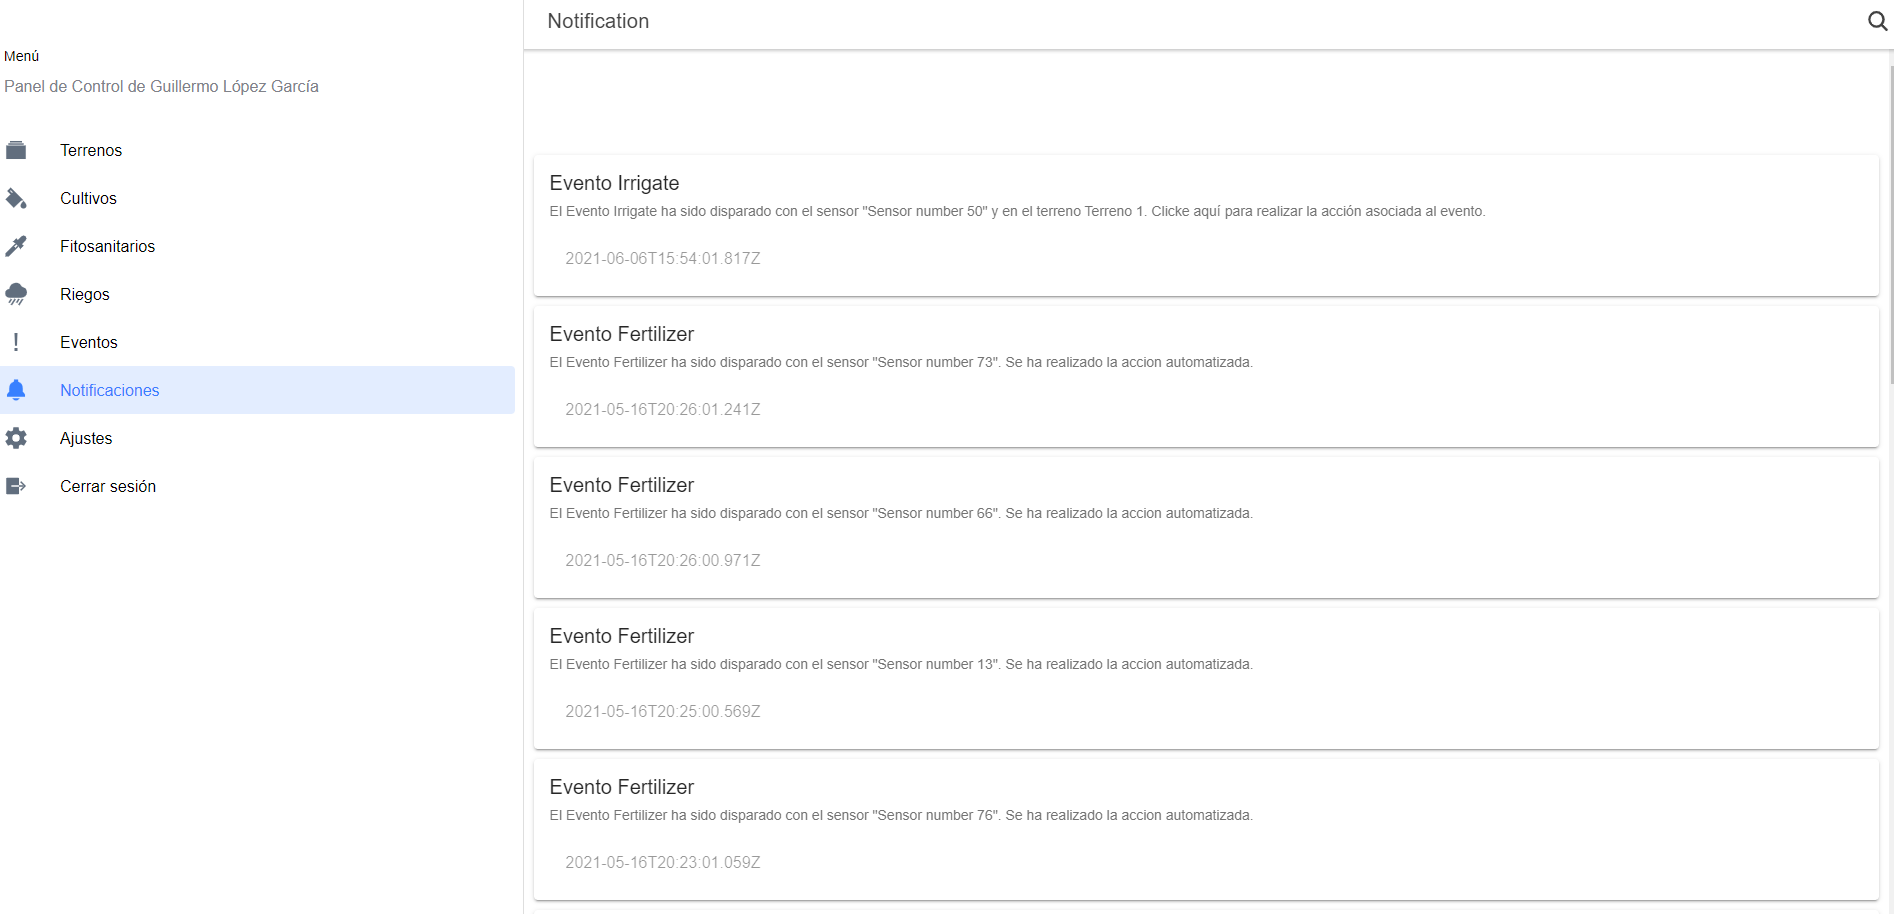
\includegraphics[width=0.7\linewidth]{images/user-manual/notifications/list.png}
    \caption{Listar Notificaciones}
\end{figure}

\subsubsection{Buscar}
Para buscar notificaciones, el usuario deberá pulsar en la barra superior de la sección. Una vez lo haga, el usuario deberá escribir su búsqueda. El sistema automáticamente volverá a listar las notificaciones con el filtro aplicado, como se puede apreciar en la Figura 9.31.
\begin{figure}[H]
    \centering
    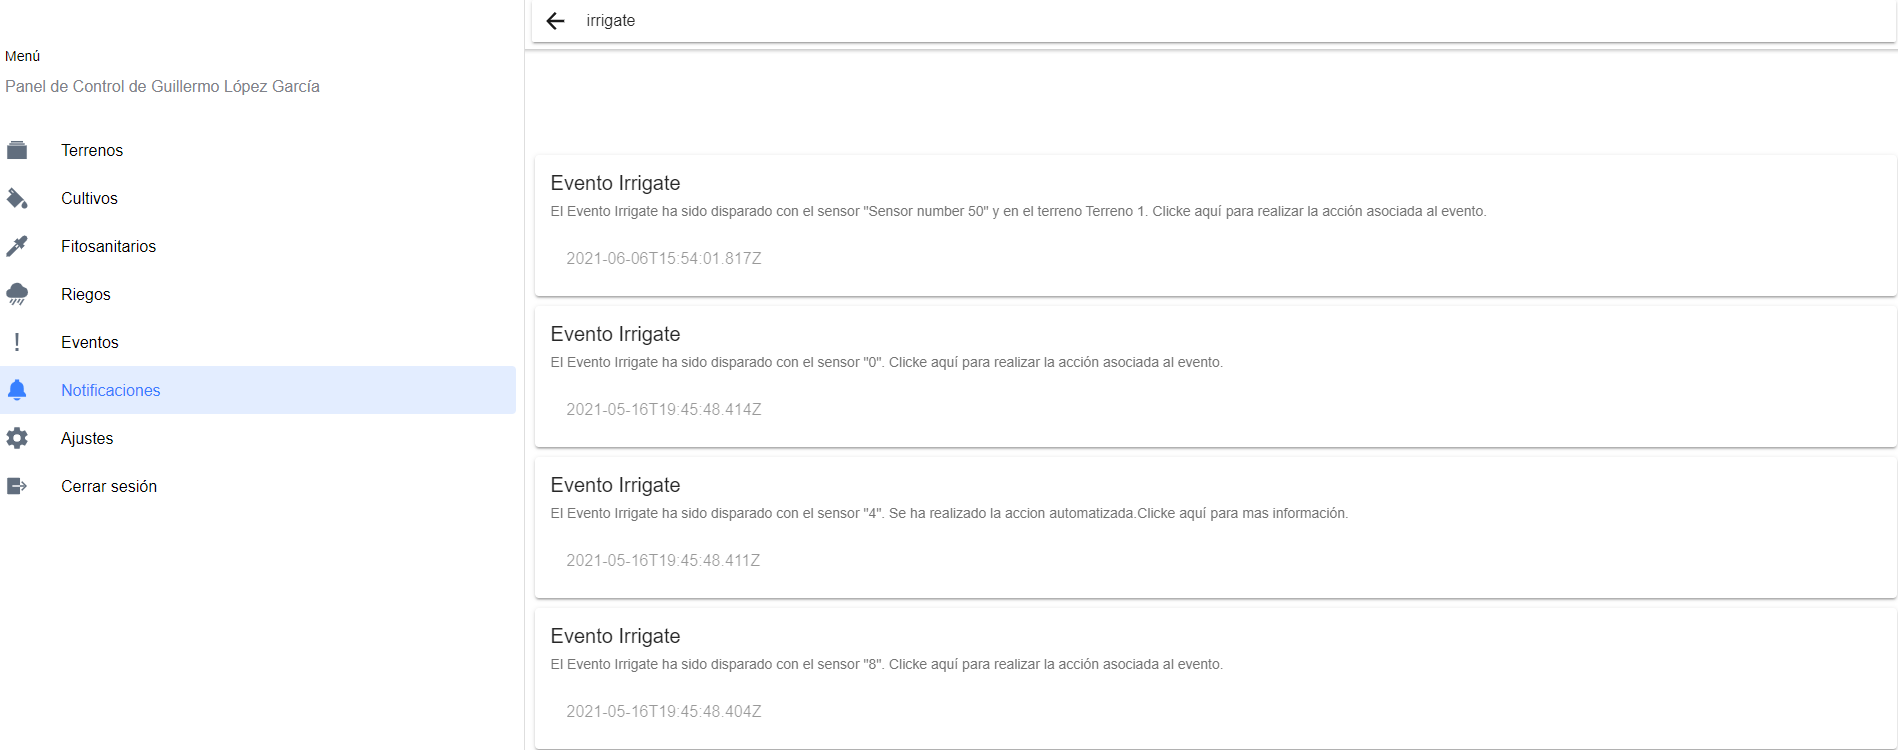
\includegraphics[width=0.7\linewidth]{images/user-manual/notifications/search.png}
    \caption{Buscar Notificaciones}
\end{figure}

\subsection{Ajustes}
En esta sección, se permite ver y modificar todos los ajustes del sistema de los usuarios.

\subsubsection{Ver}
Para ver los ajustes, el usuario deberá moverse a la sección usando el menú lateral. Una vez este en la sección, el sistema mostrará al usuario todas sus opciones de ajustes y los valores actuales. Esto se puede apreciar en la Figura 9.32.
\begin{figure}[H]
    \centering
    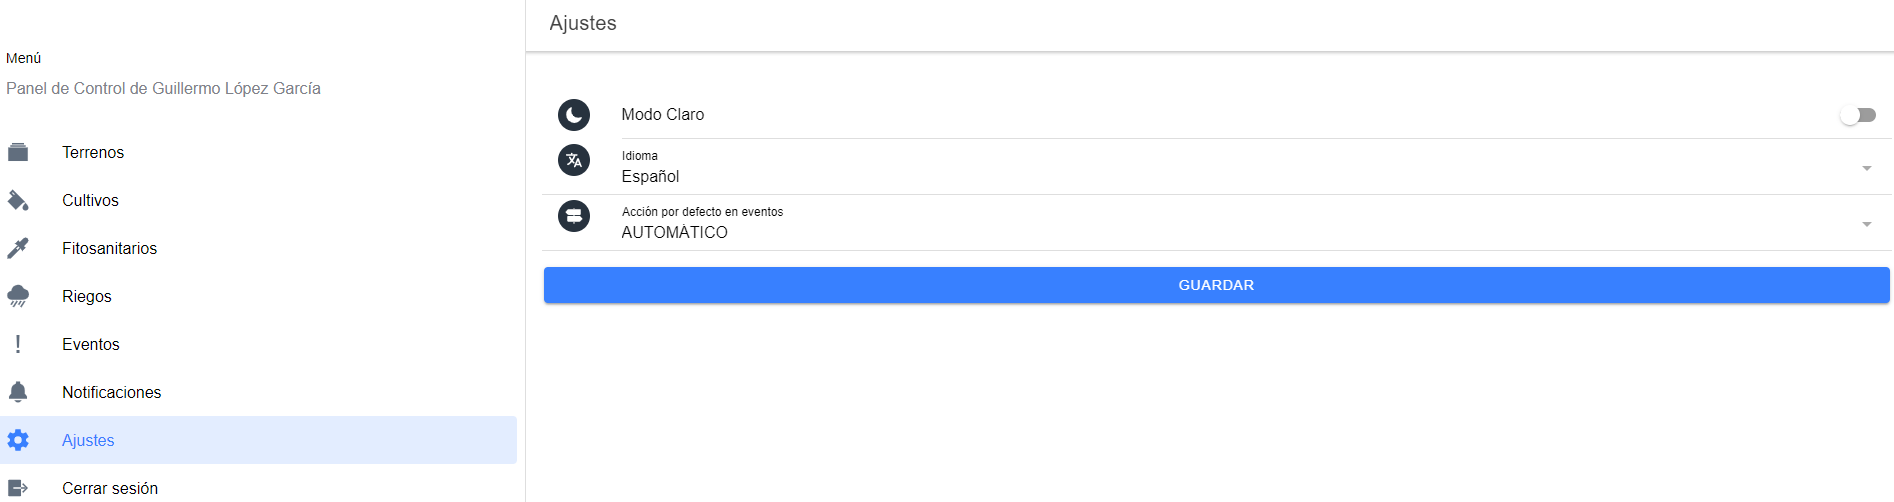
\includegraphics[width=0.7\linewidth]{images/user-manual/settings/list.png}
    \caption{Ver Ajustes}
\end{figure}

\subsubsection{Modificar}
Para modificar los ajustes del sistema, el usuario deberá entrar en la sección de ajustes y modificar los valores en los diferentes campos existentes. Una vez lo haya modificado, al pulsar sobre el botón ``Guardar'', el sistema guardará los nuevos valores de los ajustes del sistema del usuario, como se aprecia en la Figura 9.33.
\begin{figure}[H]
    \centering
    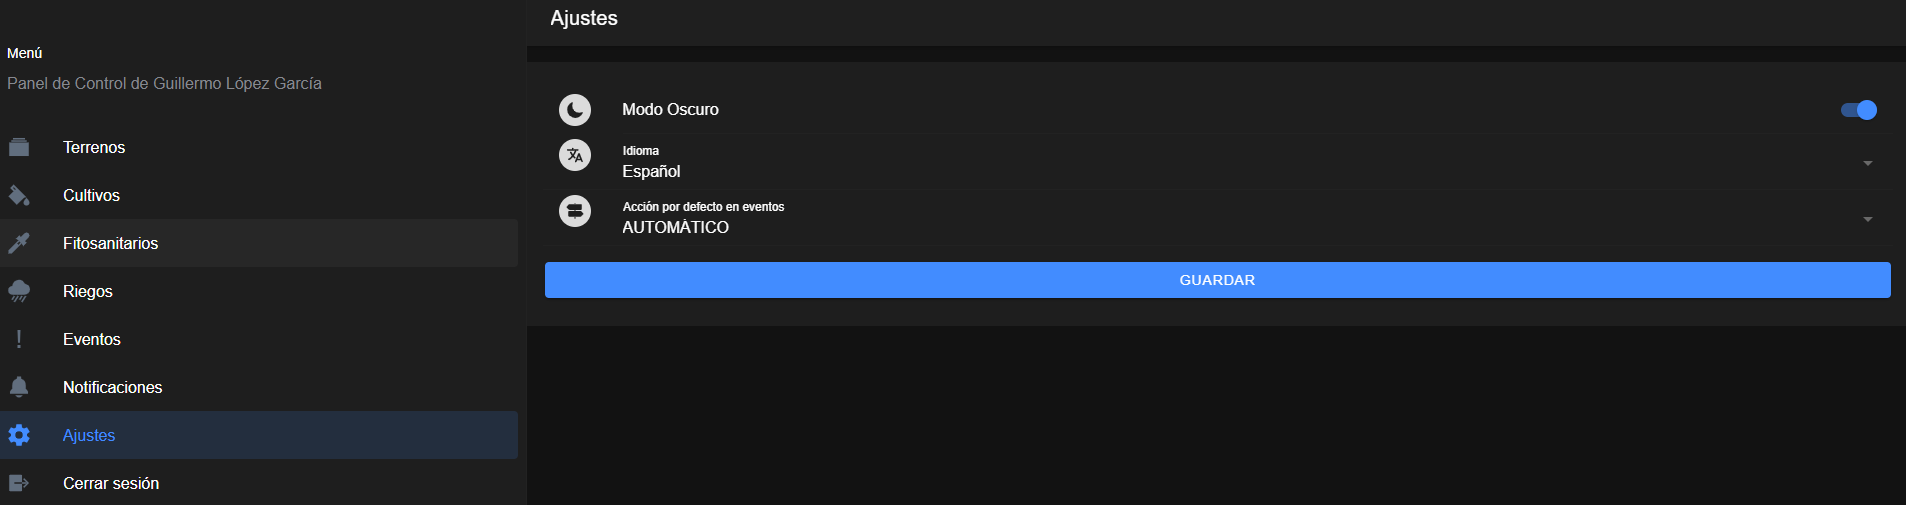
\includegraphics[width=0.7\linewidth]{images/user-manual/settings/update.png}
    \caption{Actualizar Ajustes}
\end{figure}
\end{document}
